
% load the document class KOMA-Script Report
\documentclass[	
		a4paper,			% Papierformat waehlen
		12pt,				% Schriftgroesse
%		BCOR5mm,			% Bindungskorrektur
%		draft,				% Randueberschreitungen werden schwarz markiert
%		DIV13,				% Unterteilung des Blatts in DIVxx - xx Teile              OBSOLETE
						% Je kleiner die Zahl umso groesser die Raender
						% Um Optimale Anpassung zu erhalten : DIVcalc + \typearea...
%		BCOR5mm,			% Bindekorrektur BCORXmm - Xmm breit                       OBSOLETE
		%pointlessnumbers,		% KEIN ZWEITER PUNKT IN DER NUMMERIERUNG DER ÜBERSCHRIFTET 2.2 statt 2.2.	
%
%      KOPF/FUSSZEILE
%		headinclude,			% Head gehoert mit zum Textblock/auskommentiert im Seitenrand
		headsepline,			% Trennlinie zwischen Kopf und Text, schaltet automatisch 
						% headinclude mit ein
%		footinclude,			% wie Head nur Foot
%		footsepline,			% wie headsepline
%
%      LAYOUTPARAMETER
%		twocolumn,			% Zweispaltige Texte
		onecolumn,			% Einspaltig
%		twoside,			% Zweiseitiger Druck re -li sind gespiegelt vom Satzspiegel
		oneside,			% Einseitig
%		openright,			% Sollte bei zweiseitigem Druck eignestellt werden
%		cleardoublestandard		% Alles fuer 2Seitige mit openright: Kolumnentitel linke Seite
%		cleardoubleplain		% nur Seitenzahlen linke Seite
%		cleardoubleempty		% linke Seite ganz leer
%		chapterprefix,			% Kapitel wir zu beginn eines Kapitels ausgegeben
%		appendixprefix,			% Anhang wird vor Kapiteln im Anhang ausgegeben
		headings=normal,		% kleine ueberschriften, oder small-, oder big-headings.
						% Standard ist Big
%
%	TABELLENEIGENSCHAFTEN
		captions=tableheading,		% Um richtigen Abstand fuer Ueberschrift zu erhalten, 
						% Ueberschrift wird genommen
%
%	VERZEICHNISEINSTELLUNGEN
%		tocleft,			% Setzt das Inhaltverzeichnis nicht eingerueckt nach links
%		liststotoc,			% Abb.- und Tab.Verzeichnisse ins Inhaltsverzeichnis
%		liststotocnumbered, 		% wie liststotoc nur mit Gliederungspunktangabe
%		bibtotoc,			% Literaturverzeichnis ins Inhaltverzeichnis
%		bibtotocnumbered,		% s.o. nur mit Gliederungsebene
%		idxtotoc,			% Eintrag ins Inhaltsverzeichnis fue Index
%		openbib,			% Veraendert aussehen des Lit.-Verzeichnisses
%	Language
%		ngerman,			% to pass as standard to all packages
%halfparskip,                                         % Europäischer Satz: Abstand zwischen Absätzen
%	abstracton,																					 % Spezielle Formatierung, die erlaubt, dass die
																											 % Zusammenfassung vor dem Inhaltsverzeichnis steht
	%draft,		 % Es handelt sich um eine Vorabversion	
%	final		 % Es handelt sich um die endgültige Version
]{scrreprt}

% load packages for european, espacially german users

\usepackage[T1]{fontenc}			% Schriften fuer Europaeische Zeichen passend Kodiert
\usepackage[utf8]{inputenc}        		% Eingabe von Umlauten, ss usw. - 
						% utf8: kann nicht jeder Editor speicher, aber plattformuebergreifend
						% latin1: Unix, VMS, Windows
						% ansinew: Windows
						% latin9: wie latin1, jedoch mit Eurozeichen
						
\usepackage[					% Passt Konventionen an Sprache an
	     english, 
	     ngerman				% ngerman: Neue Deutsche Rechtschreibung
	    ]{babel}				% z.B. UKenglish, USenglish, canadian, german, austrian, naustrian
	    
%\usepackage[latin1]{inputenc}                   % direkte Umlauteingabe (ä statt "a)
                                                % latin1/latin9 für unixoide Systeme
                                                % (latin1 ist auch unter Win verwendbar)
                                                % ansinew für Windows
                                                % applemac Macs
                                                % cp850 OS/2
\usepackage{times}              	        % Schriften Paket
\usepackage{array,ragged2e} 			% Wichtig für Abstandsformatierung
%---------------------------------------------------------------------------------------------------
\usepackage{cmbright}                                  % serifenlose Schrift als Standard
                                                       % + alle für TeX benötigten mathematischen
                                                       %   Schriften einschließlich der AMS-Symbole
\usepackage[scaled=.90]{helvet}                        % skalierte Helvetica als \sfdefault
\usepackage{courier}                                   % Courier als \ttdefault
%---------------------------------------------------------------------------------------------------
%\usepackage[automark]{scrpage2}                        % Anpassung der Kopf- und Fußzeilen
\usepackage{xspace}                                    % Korrekter Leerraum nach Befehlsdefinitionen
\usepackage{setspace}				  % Dieses Package brauchen wir für den 				
\usepackage[pdftex]{graphicx}
\usepackage[absolute,overlay]{textpos}         

%\usepackage{natbib}                                    % Neuimplementierung des \cite-Kommandos
\usepackage{bibgerm}       				 % Deutsche Bezeichnungen
\usepackage[final]{pdfpages}                           % include pages of external PDF documents

%\usepackage{makeidx}					% Paket zur Erstellung eines Stichwortverzeichnisses
%\makeindex						 % Automatische Erstellung des Stichwortverzeichnis
%\usepackage[intoc,
%						german,
%						prefix]{nomencl}
%\makenomenclature
	    
%\hyphenation{}					% Trennung von Woertern falls nicht automatisch korrekt erkannt
%\usepackage{icomma}				% Bei deutscher Schreibweise, damit keine

%\usepackage[scaled=0.66]{luximono}		% Schrift fuer Typewriter - Quellcode ~8pt
				

% Fuer optimale Anpassung des Satzspiegels
%\typearea[current]{calc}			% Bestimmt Rasterzahl aus Schriftgroesse und Anzahl der 		
						% Zeichen/Woerter pro Zeile

% FUSS UND KOPFZEILENANPASSUNG
%\pagestyle{plain}				% empty: Keine Kopf/Fusszeile
						% plain: Seitenzahl am Fussende
						% headings: aktiviert lebende Kolumnentitel (Kapitel im Kopf)
						% myheadings : eigene Kopf- fußzeilen
						% fancy: Erlaubt die Verwendung der in dem Paket "fancyhdr" 
						% definierten Befehle zur Erstellung eigener Kopf- und Fußzeilen

%%error
% scrpage2 ist obsolete!
%\usepackage[
%	    automark				% takes the chapter variant
%	   ]{scrpage2}				% Fuer eigene Kopf/Fusszeilen, ermoeglicht. 
% stattdessen scrlayer-scrpage:

\usepackage{scrlayer-scrpage}
\pagestyle{scrheadings} %, scrplain}
\clearscrheadings				% clear old header style
\clearscrplain					% clear plain header style
\clearscrheadfoot				% clear foot style
\automark[chapter]{chapter}
\ohead{\pagemark}				% beide Außenseiten des Headers --Seitenzahl
\ihead{\headmark}				% beide Innenseiten Headers -- Chapter

%\chead						% zentriert 
%\lehead					% left even
%\cehead
%\rehead
%\lohead					% left odd
%\cohead
%\rohead
%%


%\lehead{\leftmark}
%\lohead{\rightmark}
%\ofoot[\pagemark]{}				% auf plain seiten Seitenzahl außen
									
% Schriftfamilien Laden
\usepackage{lmodern}				% Laedt die Schriftart Latin-Modern fuer Text
\usepackage{textcomp}
%\usepackage{courier}
%\rmfamily
%\sffamily
%\ttfamily
%\renewcommand{\rmdefault}{
%			  pbk	% Bookman
%			  phv	% Helvetica
%			  cmr	% CM Roman
%			  ppl	% Palatino
%			  ptm	% Times Roman
%			  pag	% Avant Garde
%			  pcz	% Zapf Chancery
%			 }
%\renewcommand{\familydefault}{\sfdefault}

% Alternativ Schriftart (Textshchrift) ändern über usepackage:
%\usepackage{
%	    mathpazo	% Palatino
%	    mathptmx	% Times
%	    avant	% Avant Garde
%	    courier	% Courier
%	    chancery	% Zapf Chancery
%	    bookman	% Bookman
%	    newcent	% New Century Schoolbook
%	    charter	% Charter
%	    helvet	% Helvetica
%} 
%\usepackage[scaled=0.92]{helvet}		% Helvetica, ist größer als Times und sollte bei verwendung beider skaliert werden.

% Im Dokument wechslen:
%\fontfamily{pbk}\selectfont

\usepackage[
	    babel,
%	    german=guillemets,  		% franz. <<  >>
	    german= quotes,			% deutsche Anfuehrungszeichen "
	   ]{csquotes}				% Laden der richtigen Anfuehrungszeicehn fuer deutsche sprache
						% = quotes fuer englische sprache



	   
%\usepackage{setspace}				% Fuer Abstaende im Dokument
%\onehalfspacing				% aendert Zeilenabstand auf 1 1/2
									
%\usepackage{microtype}				% optischer Randausgleich in PDF's
									% ungeeignet fuer internettexte o.ae.	
	   
%\usepackage[					% Papierformate auf denen gedruckt werden soll
%		a0,b0,
%		a1,b1,
%		a2,b2,
%		a3,b3,
%		a4,b4,
%		a5,b5,
%		a6,b6,
%		letter,
%		legal,
%		executive,
%		center,				% zentrierter druck
%		landscape,			% querformat
%		]{crop}
	 
									
\usepackage[a4paper]{geometry}			% Anpassung von Seitenraender per Hand
\geometry{					% Wenn Zweiseitig-> left->inner : right->outer	
	    top=2cm, 				% Weitere Moeglichkeiten: height - Texthoehe, width - Textbreite
	    bottom=5cm,
	    inner=2cm,
	    outer=3cm
         }	

\setlength{\headheight}{1.5cm}
\setlength{\voffset}{0.5cm}


\usepackage[					% To set Text at a specific 
		absolute,			% absolute - absolute position on the page
		overlay,			% overlay - if using absolute option text is placed below other things
%		showboxes,			% showboxes - shows boxes around the text
%		noshowtext,			% noshowtext - just show the box if it is on
%		verbose,			% verbose - package writing things to output like calculations
%		quiet,				% quiet turns this off : verbose = default
	    ]{textpos}

\usepackage[
	    hyperref 	= false,		% switch off hyperref hack
	    float 	= true,			% switch off float hack
	    listings 	= true,  		% switch off listings hack
	   ]{scrhack}				% to get rid off the warning @addtocbasic

	   
%\usepackage{anyfontsize} % hilft gegen font shape not available, was wegen \DeclareMathSizes auftreten kann
\usepackage{relsize}                            % für größere und kleinere Gleichungen über den Befehl \mathlarger bzw. \mathsmaller, auch \textlarger und \textsmaller

\usepackage{lscape}

%---------------------------------------------------------------------------------------------------
% Anpassung der Parameter, die TeX bei der Berechnung der Zeilenumbrüche verwendet:
%---------------------------------------------------------------------------------------------------
\tolerance 1414
\hbadness 1414
\emergencystretch 1.5em
\hfuzz 0.3pt
\widowpenalty=10000
\vfuzz \hfuzz
\raggedbottom

\usepackage{color}				% to use colors, espacially for source codes
\usepackage[%
%	    table				% Zum automatischen Laden des Pakets colortbl - fuer Tabellen
	   ]{xcolor}				% for Hyperref package, that one can say red than rgb values

	   
	   
\definecolor{mygreen}{rgb}{0,0.6,0}
\definecolor{forestgreen}{rgb}{0.0, 0.27, 0.13}
\definecolor{mygray}{rgb}{0.5,0.5,0.5}
\definecolor{mymauve}{rgb}{0.58,0,0.82}
\definecolor{lila}{rgb}{0.6, 0.4, 0.8}
\definecolor{lavendel}{rgb}{0.75, 0.58, 0.89}
\definecolor{applegreen}{rgb}{0.55, 0.71, 0.0}
\definecolor{azure}{rgb}{0.0, 0.5, 1.0}
\definecolor{yellow}{rgb}{0.99, 0.93, 0.0}
\definecolor{brown}{rgb}{0.59, 0.29, 0.0}
\definecolor{cinnamon}{rgb}{0.82, 0.41, 0.12}
\definecolor{pumpkin}{rgb}{1.0, 0.46, 0.09}
\definecolor{pink}{rgb}{0.91, 0.25, 0.78}

\definecolor{DOGGYbg}{RGB}{80,90,100} %HAW Color
\definecolor{DOGGY}{RGB}{26,60,116} % HAW Color 2
\definecolor{lgray}{RGB}{240,240,240} %HAW Color
\definecolor{darkgreen}{RGB}{50,150,50} %HAW Color

\definecolor{brightgray}{RGB}{230,230,230}

\newcommand{\boxColorForOne}{black}
\newcommand{\boxColorForZero}{lightgray}
\newcommand{\boxColorForSqrt}{green}

\newcommand{\textColorForOne}{white}
\newcommand{\textColorForZero}{black}
\newcommand{\textColorForSqrt}{black}

\newcommand{\boxHeightL}{7}
\newcommand{\boxWidthL}{7}
\newcommand{\boxHeightS}{7}
\newcommand{\boxWidthS}{7}
\newcommand{\boxWidthWide}{7}
\newcommand{\boxHeightHigh}{7}



\newcommand{\myboxOnePos}{\colorbox{\boxColorForOne}{\makebox(\boxWidthL,\boxHeightL){\textcolor{\textColorForOne}{}}}}
\newcommand{\myboxOneNeg}{\colorbox{\boxColorForOne }{\makebox(\boxWidthL,\boxHeightL){\textcolor{\textColorForOne}{-}}}}
\newcommand{\myboxZero}  {\colorbox{\boxColorForZero}{\makebox(\boxWidthL,\boxHeightL){\textcolor{\textColorForZero}{}}}}
\newcommand{\myboxSqrtPos}{\colorbox{\boxColorForSqrt}{\makebox(\boxWidthL,\boxHeightL){\textcolor{\textColorForSqrt}{}}}}
\newcommand{\myboxSqrtNeg}{\colorbox{\boxColorForSqrt}{\makebox(\boxWidthL,\boxHeightL){\textcolor{\textColorForSqrt}{-}}}}

\newcommand{\myBlackBox}{\colorbox{black}{\makebox(\boxWidthS,\boxHeightS){\textcolor{\textColorForSqrt}{}}}}
\newcommand{\myGrayBox}{\colorbox{gray}{\makebox(\boxWidthS,\boxHeightS){\textcolor{\textColorForSqrt}{}}}}
\newcommand{\myLightgrayBox}{\colorbox{lightgray}{\makebox(\boxWidthS,\boxHeightS){\textcolor{\textColorForSqrt}{}}}}
\newcommand{\myDarkgrayBox}{\colorbox{darkgray}{\makebox(\boxWidthS,\boxHeightS){\textcolor{\textColorForSqrt}{}}}}

\newcommand{\myBlackBoxHigh}{\colorbox{black}{\makebox(\boxWidthS,\boxHeightHigh){\textcolor{\textColorForSqrt}{}}}}
\newcommand{\myBlackBoxWide}{\colorbox{black}{\makebox(\boxWidthWide,\boxHeightS){\textcolor{\textColorForSqrt}{}}}}
\newcommand{\myLightgrayBoxHigh}{\colorbox{lightgray}{\makebox(\boxWidthS,\boxHeightHigh){\textcolor{\textColorForSqrt}{}}}}
\newcommand{\myLightgrayBoxWide}{\colorbox{lightgray}{\makebox(\boxWidthWide,\boxHeightS){\textcolor{\textColorForSqrt}{}}}}

\usepackage{tcolorbox} 

\newtcolorbox{mytextbox}[1]{%
    tikznode boxed title,
    enhanced,
    arc=0mm,
    interior style={white},
    attach boxed title to top left= {xshift=0.5cm, yshift=-\tcboxedtitleheight/2},
    fonttitle=\bfseries,
    colbacktitle=white,coltitle=black,
    boxed title style={size=normal,colframe=gray,boxrule=0pt},
    title={#1}}
\usepackage[%
%	    leqno,				% Nummern linksbuendig
%	    reqno,				% Nummern rechtsbuendig (Standard)
%	    fleqn,				% Gleichungen linksbuendig statt zentriert
	   ]{amsmath}
\usepackage{amsfonts}				% Um Zahlenraeume richtig darzustellen
\usepackage{mathtools}


% Betragsstriche über \abs, Doppelbetragsstriche über \norm
\DeclarePairedDelimiter\abs{\lvert}{\rvert}%
\DeclarePairedDelimiter\norm{\lVert}{\rVert}%

\usepackage[%
	    thinlines,				% dünne linien
%	    thicklines,				% dicke linien
	   ]{easybmat}				% For Matrices with dottet lines between fields, horizontal or vertical
%\usepackage{MnSymbol}				% Zusaetzliche Zeichen
\usepackage{trsym}				% Fuer Laplace-Fourier-Symbole
\usepackage{mathrsfs}				% Fuer Matheschrift
\usepackage{xfrac}
\usepackage{nicefrac}
\usepackage{esint}
%\usepackage{exscale} % lässt Klammern in Gleichungen verschwinden!!
%\DeclareMathSizes{10.95}{30}{15}{15} % 10.95 für 11pt in documentclass

\def\mathunderline#1#2{\color{#1}\underline{{\color{black}#2}}\color{black}}

\usepackage{soul}

\usepackage[%				
%	    group-separator 	= {.}, 		% group-seperator={,} -> 1,345,234.23
%   	    round-mode 		= places,		% round-mode= places(2digits), figures(1digit)
%	    round-precision 	= 3,		% round-precision= x , xdigits are rounded to
	    binary-units 	= true,		% Laden von \byte \bit, \kibi usw. (false default)
	    locale 		= DE,		% lacale= DE, uses german
	    per			= slash,
	    alsoload            = binary,
%	    loctolang		={
%				  UK:english, 
%				  DE:ngerman
%		      		 },		% loctolang={USA:USenglish,DE:ngerman}, if language changed in document
	    detect-all				% detect-all : uses the text options not the math mode to set the letters/numbers
	   ]{siunitx}

\usepackage{graphicx} 				% für Grafik-Einbindung
%\usepackage{subfigure}				% Für Untergrafiken, wenn eine eigene Bildunterschrift erwuenscht
\usepackage{subcaption}
\usepackage[hypcap=false]{caption}				% für Captions bei Grafiken ohne figure Umgebung wie in Minipage nötig
\usepackage[%
	    update				% if pdf conversion is older than eps file, new conversion is done
	   ]{epstopdf}				% eps to pdf needs for pdflatex - after graphicx

%\usepackage{subfig}
\usepackage{capt-of}

%---------------------------------------------------------------------------------------------------
% Abbildungsverzeichnis
%---------------------------------------------------------------------------------------------------
%\graphicspath{{img/}}

\usepackage{tikz}
%\usepackage{background}
\usetikzlibrary{thedecorations, arrows,shapes, automata, positioning, calc, backgrounds, decorations.pathreplacing}


\newcommand{\tikzmark}[1]{\tikz[overlay, remember picture] \coordinate (#1);}

\tikzset{node/.style={draw,shape=circle}}
\newcommand{\order}[2][th]{\ensuremath{{#2}^{\mathrm{#1}}}}
\usepackage{multirow}				% Fuer Mehrzeilige Zellen
\usepackage{multicol}
%\usepackage{array}					% Festlegen von Breiten, Präfixe, Suffixe
% see also package siunitx - damit Spalten mit Zahlen auf bestimmte Länge ausgerichtet werden
\usepackage{tabularx}				% Zum festlegen der Gesamtbreite der Tabelle & verwenden von X fuer 
									% variable Spaltenbreite
%\usepackage{longtable}				% Tabelle ueber mehr als eine Seite
\usepackage{ltxtable}				% longtable + tabularx eigenschaften

%\usepackage{rotating}				% Querformat der Tabelle
									% !!! Vorsicht !!!
									% tablecaptionabove wird nicht ausgewertet,
									% Einfuegen von \vskip\abovecaptionskip --> Nur unter KOMA Script
\usepackage{ctable}					% For tables with footnote under the table directly


\setlength{\arraycolsep}{0.4pt}
\delimitershortfall=0pt % Höhereduzierung der Klammern von Matrizen gegenüber dem Inhalt

\usepackage{tabu} % fuer farbige Zeilen in Tabellen
\usepackage[  % Packet ist jetzt glossaries-extra statt glossaries - keine Ahnung, ob die es die auskommentierten Optionen gibt!
	    xindy,%={language=german-modern, codepage=utf8},
	    automake,				
	    numberedsection,
%	    toc,      				% Fügt Eintrag ins Inhaltsverzeichnis hinzu, defualt false
	    nonumberlist,			% keine Ausgabe der Seitenzahlen
%	    nowarn,				% unterdrückt alle warungen des pakets
%	    nomain,				% kein hauptglossary wird erzeugt, acronym oder newglossary um Einträge zu erzeugen
%	    sanitize={%				% unterdrückt die keys für einträge oder fügt sie hinzu
%	    name        = false,%
%	    description = false,%
%	    symbol      = false},%
%	    translate = true,			% zur übersetzung von einträgen - siehe doku, default false
	    hyperfirst = true,			% erzeugt hyperlink zum glossar bei erster verwendung, default true
%	    hyper = false,			% Hyperlinks ausschalten
%	    numberline,				% Eintrag ins toc mit Nummerierung
%	    section=section,			% in welcher ebene der eintrag, default chapter if loaded sonst section
%	    style = long,			% default list, sonst: long, super, tree
%	    nolong,				% pakete für longtable werden nicht geladen und befehle nicht definiert
%	    nosuper,				% supertabular wird nicht geladen, pakete nicht definiert
%	    nolist,				% list wird nicht geladen definiert
%	    notree,				% gloassrytree wird nicht geladen definiert
%	    nostyles,				% keine styles werden geladen, eigene definieren
%	    counter = page,			% page default, or any other counter
%	    sort = def,				% def - sortiert nach definition, standard(default)-sortiert nach sort key, sonst name, use - sortieren nach reihenfolge wie sie im dokument vorkommen
%	Acronym options
%	    acronym,  				% Seperate Liste für Acronyme zum Glossary, default - false
%	    acronymlist={},			% wenn mehr als eine abkürzungsliste, muss diese hier mit angegeben werden damit das glossary als acronym behandelt wird
%	    description,			% erlaubt eine zusätzliche beschreibung
%	    footnote,				% schreibt die long version als fußnote bei erster nutzung
%	    smallcaps,				% acronyme werden als kapitelchen angezeigt
%	    smaller,				% kleinere schrift, laden von relsize für befehl textsmaller erforderlich
%	    dua,				% langform wird immer ausgegeben
	    shortcuts,				% um selbe befehle wie acronym paket zu haben
	   ]{glossaries-extra}		


\GlsSetXdyCodePage{duden-utf8}

% sorgt dafür, dass die Erklärungen alle gleich eingerückt sind
\setglossarystyle{long}
\renewcommand{\glsnamefont}[1]{\textbf{#1}}

% Bachlorarbeit.gls erzeugen:
% $ cd Bachelorarbeit
% $ makeglossaries "Bachelorarbeit"

\makeglossaries 

\newabbreviation{1d-dft}{1D-DFT}{eindimensionale diskrete Fouriertransformation}
\newabbreviation{1d-dftn}{1D-DFT}{eindimensionalen diskreten Fouriertransformation}
\newabbreviation{2d-dft}{2D-DFT}{zweidimensionale diskrete Fouriertransformation}
\newabbreviation{2d-dftn}{2D-DFT}{zweidimensionalen diskreten Fouriertransformation}

\newabbreviation{adc}{ADC}{Analog Digital Converter}
\newabbreviation{adu}{ADU}{Analog Digital Umsetzer}
\newabbreviation{amr}{AMR}{anisotroper magnetoresistiver Effekt}
\newabbreviation{amr2}{AMR}{anisotropen magnetoresistiven Effekt}
\newabbreviation{asic}{ASIC}{Application Specific Integrated Circuit, \textit{dt.: Anwendungsspezifischer Integrierter Schaltkreis}}

\newabbreviation{dac}{ADC}{Digital Analog Converter}
\newabbreviation{dau}{ADU}{Digital Analog Umsetzer}
\newabbreviation{dct}{DCT}{diskrete kosinus Transformation}
\newabbreviation{dft}{DFT}{diskrete Fouriertransformation}

\newabbreviation{idft}{IDFT}{inverse diskrete Fouriertransformation}
\newabbreviation{isar}{ISAR}{Integrated Sensor Array}

\newabbreviation{ft}{FT}{Fouriertransformation}
\newabbreviation{fft}{FFT}{Fast Fouriertransformation}

\newabbreviation{lsb}{LSB}{Least Significant Bit}

\newabbreviation{msb}{MSB}{Most Significant Bit}

\newabbreviation{ram}{RAM}{Random Access Memory}

\newabbreviation{tmr}{TMR}{tunnelmagnetoresistiver Effekt}
\newabbreviation{tmr2}{TMR}{tunnelmagnetoresistiven Effekt}



\glsaddall

\setlength\LTleft{0pt}
\setlength\LTright{0pt}
\setlength\glsdescwidth{0.8\hsize}


% Hyperref for PDFLATEX with links    
\usepackage[
	    draft 	= false,			% all hypertext options are turned off
	    final 	= true, 			% all hypertext options are turned on
	    raiselinks 	= true,				% Allow links to reflect real height - e.g. with pictures
	    breaklinks	= false,			% false=Do not break a line within a link
	    backref	= false,			% false=no backlinks in the bibliography
	    pagebackref = false,			% false=no pagebacklinks in bibliography
%	    linktocpage = true,				% true=makes page-no linked and not text in TOC,LOF and LOT
	    linktoc	= all,
%			  none,
%			  section,
%			  page,
	    colorlinks	= false,			% true=Colors the text of links and anchors
%	    linkcolor 	= red, 				% Color for normal internal links.
%	    anchorcolor = black, 			% Color for anchor text.
%	    citecolor 	= green, 			% Color for bibliographical citations in text.
%	    filecolor 	= cyan, 			% Color for URLs which open local files.
%	    menucolor 	= red,				% Color for Acrobat menu items.
%	    runcolor 	= filecolor,			% Color for run links (launch annotations).
%	    allcolors 	= red,				% Set all color options (without border and field options).
	    urlcolor 	= blue,				% Color for linked URLs.
%	    allbordercolors  =red,			% Set all colors
%	    citebordercolor =green,			% cite color
%	    filebordercolor =cyan,			% file color
%	    linkbordercolor =red,			% link color
%	    urlbordercolor  =blue,			% url color
%	    pdfborder = 0 0 0,				% weder farbige links noch umrandung			
%	    menubordercolor =red,			% set menu color
%	    frenchlinks = 	false,			% Use small caps instead of color for links.
	    bookmarks	=	true,			% true=Bookmarks are added to the pdf
	    bookmarksopen=	false,			% false=Bookmarks not open when opening the pdf
	    bookmarksnumbered=true,			% true= Eintraege sind nummeriert
%	    pdfpagemode	=	FullScreen,		% File is opened in Full Screen
%	    pdfstartview=	fit,			% Fit size when opening pdf
	    pdfpagelabels=	true,			% true = Roemische Zahlen usw werden dargestellt,
							% false= fortlaufende nummerierung
	   ]{hyperref}
\hypersetup{hidelinks}

\usepackage{listings}					% options : basicstyle= e.g. \ttfamily
							% fontadjust=true % before load package [scaled=0.78]{luximono}
							% columns=flexible

\lstset{ %
  backgroundcolor=\color{white},   % choose the background color; you must add \usepackage{color} or \usepackage{xcolor}; should come as last argument
  basicstyle=\footnotesize,        % the size of the fonts that are used for the code
  breakatwhitespace=false,         % sets if automatic breaks should only happen at whitespace
  breaklines=true,                 % sets automatic line breaking
  captionpos=b,                    % sets the caption-position to bottom
  commentstyle=\color{mygreen},    % comment style
  deletekeywords={...},            % if you want to delete keywords from the given language
  escapeinside={\%*}{*)},          % if you want to add LaTeX within your code
  extendedchars=true,              % lets you use non-ASCII characters; for 8-bits encodings only, does not work with UTF-8
  frame=single,	                   % adds a frame around the code
  keepspaces=true,                 % keeps spaces in text, useful for keeping indentation of code (possibly needs columns=flexible)
  keywordstyle=\color{blue},       % keyword style
  language=VHDL,                 % the language of the code
  morekeywords={*,...},            % if you want to add more keywords to the set
  numbers=none,                    % where to put the line-numbers; possible values are (none, left, right)
  numbersep=5pt,                   % how far the line-numbers are from the code
  numberstyle=\tiny\color{mygray}, % the style that is used for the line-numbers
  rulecolor=\color{black},         % if not set, the frame-color may be changed on line-breaks within not-black text (e.g. comments (green here))
  showspaces=false,                % show spaces everywhere adding particular underscores; it overrides 'showstringspaces'
  showstringspaces=false,          % underline spaces within strings only
  showtabs=false,                  % show tabs within strings adding particular underscores
  stepnumber=2,                    % the step between two line-numbers. If it's 1, each line will be numbered
  stringstyle=\color{mymauve},     % string literal style
  tabsize=2,	                   % sets default tabsize to 2 spaces
  title=\lstname                   % show the filename of files included with \lstinputlisting; also try caption instead of title
  literate=
  {á}{{\'a}}1 {é}{{\'e}}1 {í}{{\'i}}1 {ó}{{\'o}}1 {ú}{{\'u}}1
  {Á}{{\'A}}1 {É}{{\'E}}1 {Í}{{\'I}}1 {Ó}{{\'O}}1 {Ú}{{\'U}}1
  {à}{{\`a}}1 {è}{{\`e}}1 {ì}{{\`i}}1 {ò}{{\`o}}1 {ù}{{\`u}}1
  {À}{{\`A}}1 {È}{{\'E}}1 {Ì}{{\`I}}1 {Ò}{{\`O}}1 {Ù}{{\`U}}1
  {ä}{{\"a}}1 {ë}{{\"e}}1 {ï}{{\"i}}1 {ö}{{\"o}}1 {ü}{{\"u}}1
  {Ä}{{\"A}}1 {Ë}{{\"E}}1 {Ï}{{\"I}}1 {Ö}{{\"O}}1 {Ü}{{\"U}}1
  {â}{{\^a}}1 {ê}{{\^e}}1 {î}{{\^i}}1 {ô}{{\^o}}1 {û}{{\^u}}1
  {Â}{{\^A}}1 {Ê}{{\^E}}1 {Î}{{\^I}}1 {Ô}{{\^O}}1 {Û}{{\^U}}1
  {œ}{{\oe}}1 {Œ}{{\OE}}1 {æ}{{\ae}}1 {Æ}{{\AE}}1 {ß}{{\ss}}1
  {ű}{{\H{u}}}1 {Ű}{{\H{U}}}1 {ő}{{\H{o}}}1 {Ő}{{\H{O}}}1
  {ç}{{\c c}}1 {Ç}{{\c C}}1 {ø}{{\o}}1 {å}{{\r a}}1 {Å}{{\r A}}1
  {€}{{\euro}}1 {£}{{\pounds}}1 {«}{{\guillemotleft}}1
  {»}{{\guillemotright}}1 {ñ}{{\~n}}1 {Ñ}{{\~N}}1 {¿}{{?`}}1
}

\usepackage[
	    official,
	    right				% Position of the Euro-Sign. verwendung: \euro oder \EUR{123,45}
	   ]{eurosym}


% Loading unit options                

\usepackage[%				
%	    group-separator 	= {.}, 		% group-seperator={,} -> 1,345,234.23
%   	    round-mode 		= places,		% round-mode= places(2digits), figures(1digit)
%	    round-precision 	= 3,		% round-precision= x , xdigits are rounded to
	    binary-units 	= true,		% Laden von \byte \bit, \kibi usw. (false default)
	    locale 		= DE,		% lacale= DE, uses german
	    per			= slash,
%	    loctolang		={
%				  UK:english, 
%				  DE:ngerman
%		      		 },		% loctolang={USA:USenglish,DE:ngerman}, if language changed in document
	    detect-all,				% detect-all : uses the text options not the math mode to set the letters/numbers
	   ]{siunitx}


\usepackage[Algorithmus]{algorithm} 			% deutsche notation im titel

% Zitate die in den Referenzen aufscheinen, aber nicht unbedingt im Text zitiert werden m�ssen
% Literatur, die mit \nocite oder \cite zitiert wird, mu� im .bib File erfasst werden!
\nocite{Guenther:2002}
\nocite{Lamport:1995}
\nocite{Goossens:2000}
\nocite{Kohm:2003}
\nocite{Hunt:2003}
\nocite{Boehm:2002}
\nocite{Schmatz:2004}
\nocite{Streitz:2005}
\nocite{HP:2004}
\nocite{Luede:2004}
\nocite{Demarco:1999}
\nocite{Kollakowski:2004}
\nocite{Dawson:2003}
\nocite{Poenicke:1988}
\nocite{Kruse:2000}
\nocite{Nilsson:1998}
\nocite{Heinsohn:1999}
\nocite{Luger:2001}
\nocite{Kuehnel:2001}
\nocite{Bigus:2001}
\nocite{Ferber:2001}
\nocite{Wooldridge:2002}
\nocite{KuroseRoss:2002}
\nocite{Vogt:2001}
\nocite{Roetzer:1999}
\nocite{P3P:2004}
\nocite{CPEX:2004}
\nocite{Duden:1997}
\nocite{Hoerauf:2001}
\nocite{Schirru:2004}
\nocite{Babic:2003}
\nocite{Luepke:2004}

	
\usepackage{bbding}					% to get cross and check symbol

\usepackage{enumerate}					% schicke Nummerierung

\usepackage{pdfpages}					% Zum Laden und einbinden von PDF-Seiten
\usepackage{pgfpages}
\usepackage{float}					% für floats (figures) in einer Minipage (geht nicht!!)
\usepackage{booktabs}					% Fuer besseres aussehen der Linien
\usepackage{framed}					% for use of newtheorem with a coloured box

\usepackage{titling}
\author{Thomas Lattmann}
\title{Chipimplementation einer zweidimensionalen Fouriertransformation für die Auswertung eines Sensor-Arrays}
\date{23.4.2018}
			
% INDEX ERZEUGEN - falls gewuenscht muessen beide direkt so eingebunden werden
%\usepackage{index}
%\makeindex

%\makenomenclature					% damit Symbolverzeichnis erzeugt wird

% Symbolverzeichnis erzeugen - lade dazu mit %%%%%%%%%%%%%%%%%%%%%%%%%%%%%%%%%%%%%%%%%%%%%%%%%%%%%%%%%%%%%%%%%%%%%%%%%%%%%%%
%  Author     : Dennis Schuethe        Date    : 28.12.2011                   %
%  Filename   : symbolpage.tex         Version : 1.0                          %
%  Information: This file will create the nomenclature and should be designed %
%               the way you want to. There are two options:                   %
%               1. Use the normal nomenclature which is given and created by  %
%                  the nomencl.sty -> see package declarations                %
%               2. To have more than one column for the nomenclature, then    %
%                  use the \begin{multicols}, but this cause a bad look,      %
%                  because the name is printed within the columns, better use %
%                  option 3                                                   %
%               3. Find the nomencl.sty and then rewrite the lines 160 and    %
%                  164 as it is shown below, then you need to add the         %
%                  \chapter*{\nomname} or \section*{\nomname} by yourself     %
%-----------------------------------------------------------------------------%
%  Changelog  :                                                               %
%  28.12.2011  opened this file                                               %
%              may the nomencl.sty could be changed by adding this as option, %
%              need to try a workaround                                       %
%  %
%%%%%%%%%%%%%%%%%%%%%%%%%%%%%%%%%%%%%%%%%%%%%%%%%%%%%%%%%%%%%%%%%%%%%%%%%%%%%%%


%157 \def\thenomenclature{%
%158  \@ifundefined{chapter}%
%159  {
%160    %\section*{\nomname}
%161    \if@intoc\addcontentsline{toc}{section}{\nomname}\fi%
%162  }%
%163  {
%164    %\chapter*{\nomname}
%165    \if@intoc\addcontentsline{toc}{chapter}{\nomname}\fi%
%166  }%

%\renewcommand{\nomname}{newname}	% New name for the nomenclature
%\chapter*{\nomname}				% Do the heading for this chapter(section)
% else			
% newpage							% only if chapter command is not used
%\begin{multicols}{2}				% Do multiple columns - use package multicol
\printnomenclature %[2cm] 			% Symbolverzeichnis mit breite xcm für symbole, std is 1cm
%\end{multicols} das Verzeichnis 
%\usepackage[
%	     intoc,					% Eintrag des Abkuerzungsverzeichnis
%	     notintoc,					% Kein Eintrag - default
%	     english,					% Ueberschrift in English (default)
%      	     german,					% in deutsch
%	    ]{nomencl}


% Loading label options               
\usepackage[ngerman]{varioref}		            	% To get automatic "see Section xy on page xx"
%\usepackage[german]{fancyref}		    		% same as varioref, except this is setting section automatically
							% Options in []-brackets:
							% language, e.g. english, ngerman - last entry is main-language
							% paren - sets the reference in ()-brackets
							% plain - no pagenumber in the reference
							% -----------------------------------------
							% standard prefixes used by fancyref:
							% sec, chap, part, fig, tab, enum, eq, fn
%\fancyrefchangeprefix{\fancyrefchaplabelprefix}{cha} 	% sets a new prefix for the label chap




% Pseudocode 			 %
\usepackage[noend]{algpseudocode}

\begin{document}

 \begin{titlepage}
\newgeometry{
	      left=4cm,
	      right=4cm,
	      top=5cm,
	      bottom=4cm
	    }
 \begin{center}

%{\scshape\Large Chipimplementation einer zweidimensionalen Fouriertransformation für die Auswertung eines Sensor-Arrays}
{\scshape\Large \thetitle} %shape\Large

\vspace{1cm}

{\scshape\Large \theauthor}

\vspace{1cm}

%{\scshape Matrikelnummer\\1924507}

\end{center}

%\vspace{12cm}
\vfill

\noindent Bachelorarbeit eingereicht im Rahmen der Bachelorprüfung\\ 
im Studiengang Informations- und Elektrotechnik\\
am Department Informations- und Elektrotechnik\\
der Fakultät Technik und Informatik\\
der Hochschule für Angewandte Wissenschaften Hamburg\\

\vspace{0.5cm}
\noindent Betreuender Prüfer: Prof. Dr.-Ing. Karl-Ragmar Riemschneider\\
Zweitgutachter: Prof. Dr.-Ing. Jürgen Vollmer\\

\vspace{0.5cm}
\noindent Abgegeben am 23.04.2018

\addtocounter{page}{-1}

\end{titlepage}
 \restoregeometry

 \pagenumbering{Roman} 
 \tableofcontents
 
 %\paragraph{}
 
 %\setcounter{page}{1}
 
 
 \chapter{Einleitung}
In der vorliegenden Arbeit wird eine zweidimensionale diskrete Fouriertransformation in VHDL implementiert. Diese Tätigkeit erfolgt im Rahmen des Projekts \gls{isar} an der 
HAW-Hamburg.
 \section{Motivation}
 Bisherige Analysen und Versuche wurden überwiegend auf theoretischer Ebene mit der Simulationssoftware Matlab oder anhand einer ca. 7x7\,cm großen Sensormatrix mit 64 einzelnen Sensoren in Verbindung mit
 einem an den PC angeschlossenen Microkontroller vorgenommen. Auf diese Weise können reale Messwerte ermittelt und verschiedene Szenarien getestet werden.
 
 Damit letztlich die Sensoren und alle Berechnungen auf einem \gls{asic} erfolgen können, ist als nächstes die Entwicklung der signalverarbeitenden Komponenten in einer Hardwarebeschreibungssprache geplant.
 Ziel ist ein Sensormodul, mit dem eine kontinuierliche Winkelberechnung zur Positionsbestimmung möglich ist. Dieses soll beispielsweise die Rotorlage eines Elektromotors ermitteln und die Information als digitales Nutzsignal ausgeben können. Ein wesentliches Punkt ist das Unterdrücken von Störfeldern, welche in Form von Inhomogenitäten, unter anderem hervorgerufen durch Fehlpositionierung (Ablage) und Schrägstellung des Gebermagneten und den Magnetsensoren selbst, verursacht werden. 

 Den erste Schritt der Signalverarbeitung stellt die Berechnung der zweidimensionalen dirketen Fouriertransformation der Sensorsignale dar (Abb. \ref{pic:AblaufFourier}), da sich im Fourierraum Störanteile leichter filtern lassen. Derzeit ist offen, ob anschließend der Winkel direkt berechnet werden kann oder vorher eine Rücktransforation erfolgen muss.
 

\begin{figure}[ht!]
 \centering
 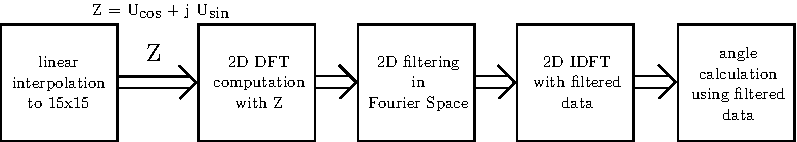
\includegraphics[width=0.8\textwidth]{img/AblaufFourier.pdf}
 \caption{Ablauf der Signalvorverarbeitung~\autocite[9]{krrts2017freqfilt}}
 \label{pic:AblaufFourier}
\end{figure}


\section{Stand der Technik}

Zur Winkelberechnung auf Basis von Magnetsensoren lassen sich verschiedene Effekte nutzen. Hierzu zählt als Vorreiter der Hall-Effekt. Weiterentwicklungen gingen über den \gls{amr2}, den \gls{gmr2} hin zum \gls{tmr2}. Sensoren die den TMR-Effekt nutzen gibt es bereits seit mehreren Jahren, es werden aber weitere Fortschritte angestrebt und erzielt. 
Die Entwicklung von Sensoren die die verschiedenen magnetoresistive Effekte nutzen, bringen Vorteile hinsichtlich des Strombedarfs, der Amplitude des Sensorsignals, Genauigkeit der Auflösung, Größe sowie benötigte Feldstärke~\autocite[2]{magSensTechOverview}. Darüber hinaus ist es nur mit den GMR- und TMR-Sensoren möglich 360${}^\circ$ aufzulösen. Die AMR-Sensoren erzeugen je Umdrehung zwei Sinusschwingungen, wodurch eine um 180${}^\circ$ versetzte Doppeldeuigkeit entsteht~\autocite{tsukakoshi2017tmrgmr}. Bei Hall-Sensoren sind die anderen genannten Schwächen deutlich stärker ausgeprägt, weswegen sie in diesem Bereich keine Verwendung finden.



%Der verwendete Prozess ist mit $\SI{350}{nm}$ im Vergleich zu modernen Prozessen mit $\SI{20}{\nm}$ oder weniger Strukturbreite um den Faktor 20 größer. Entsprechend handelt es sich um einen relativ alten Prozess.

%Kurze Beschreibung zu Standardzellen.


\section{Ziel dieser Arbeit}
Um eine Aufwandsabschätzüng einer 2D-DFT bezüglich Rechendauer und Flächenbedarf als Komponente auf einem  \gls{asic} zu erlangen, wird die Transformation auf ein Array angewandt, welches eine Größe 
hat, die sich leicht optimieren lässt. Herauszufinden, auf welche das Zutrifft, ist Teil der Arbeit. 
Es sollen Grundlagen erarbeitet werden, welche für die Transformation einer
15x15-Matrix nützlich sind. Letztere wird durch lineare Interpolation der 8x8-Sensormatrix errechnet (Abb. \ref{pic:AblaufFourier}). Von ihr ist bekannt, dass sie wegen einer vergleichsweise hohen Anzahl verschiedener Faktoren bedeutend
aufwändiger zu implementieren ist, weshalb zunächst mit einer einfacheren Berechnung Erfahrungen gesammelt und Vorarbeit geleistet werden soll.
Nach Möglichkeit soll für beide Matrixmultiplikationen, die die 2D-DFT mit der Twiddlefaktormatrix erfordert, die selbe DFT-Einheit genutzt werden. Ob und wie dies effizient erfolgen kann,
gehört ebenfalls zur Aufgabenstellung.

 
 \pagenumbering{arabic} 
 
 \chapter{Grundlagen}
 \section{Binäre Zahlendarstellung von Festkommazahlen}

Im Rahmen dieses Projekts wird von Ein- sowie Ausgangswerten mit einer Genauigkeit von 12 Bit ausgegangen.
Basierend auf älteren Sensoren wird von Werten im Bereich von $-2 < z < 2$ ausgegangen.
Aus diesem Grund müssen sowohl ein Ganzzahlanteil, sowie Nachkommastellen repräsentiert werden können. Wie dies gelingt, wird in den nächsten Abschnitten gezeigt.
Hierfür werden Festkommazahlen verwendet, aufgrund der Rechenoperationen haben diese dennoch unterschiedlich viele Vor- sowie Nachkommastellen.


\subsection{Integer-Zahl im 1er-Komplement}
Bei der Interpretation des Bitvektors als Integerwert im Einerkomplement werden die Bits anhand ihrer Position im Bitvektor gewichtet, wobei das niederwertigste Bit 
(LSB, least significant bit) dem Wert für den Faktor $2^0$ entspricht, das Bit links davon dem für $2^1$ und so weiter. Die Summe aller Bits, ohne das höchstwertigste, 
multipliziert mit ihrer Wertigkeit (Potenz) ergibt den Betrag der Dezimalzahl. Das höchstwertigste Bit (MSB, most significant bit) gibt Auskunft darüber, ob es sich 
um eine negative oder positive Zahl handelt, wobei eine 0 für eine positive Zahl steht. Entsprechend besagt die 1, dass die Zahl negativ ist.
Dies hat zur Folge, dass es eine positive und eine negative Null und somit eine Doppeldeutigkeit gibt. Des Weiteren wird
ein LSB an Auflösung verschenkt. Der Wertebereich erstreckt sich von $-2^{\mathrm{MSB}-1}+1\,\mathrm{LSB}$ bis $2^{\mathrm{MSB}-1}-1\,\mathrm{LSB}$

Diese Darstellung hat den Vorteil, dass sich das Ergebnis einer Multiplikation der Zahlen $a \cdot b$ und $-a \cdot b$ nur im vordersten Bit unterscheidet. Darüber hinaus
lässt sich das Vorzeichen des Ergebnisses durch eine einfache XOR-Verknüpfung der beiden MSB der Multiplikanden ermitteln. 
Die eigentliche Multiplikation beschränkt sich auf die Bits MSB-1 bis LSB.

Nachteile zeigen sich hingegen bei der Addition sowie Subtraktion negativer Zahlen. Auch hierfür gibt es schematische Rechenregeln, diese erfordern jedoch mehr 
Zwischenschritte als im Zweierkomplement. 


\subsection{Integer-Zahl im 2er-Komplement}\label{sec:Integer2erKomplement}

Bei der Interpretation als Zweierkomplement kann anhand es MSB ebenfalls erkannt werden, ob es sich um eine positive oder negative Zahl handelt. 
Hie bedeutet ein gesetztes MSB $-2^{MSB-1}$, was der negativsten darstellbaren Zahl entspricht. Hierbei sind alle anderen 
Bits auf 0. Für gesetzte Bits wird der Dezimalwert, wie beim Einerkomplement beschrieben, berechnet und auf den negativen Wert aufaddiert. Wenn das MSB nicht gesetzt
ist, wird der errechnete Dezimalwert auf 0 addiert. Auf diese Weise lassen sich Zahlen im Wertebereich von $-2^{MSB-1}$ bis $2^{MSB-1}-1 \,LSB$ darstellen. Der positive
Wertebereich ist also um ein LSB kleiner als der negative und es gibt keine doppelte Null.

Um das Vorzeichen umzukehren müssen alle Bits invertiert werden. Auf das Resultat muss abschließend 1 LSB addiert werden.

Vorteil bei dieser Darstellung ist, dass die mathematischen Operationen Addition, Subtraktion und Multiplikation direkt angewandt werden können. Unterstützt werden sie z.B. 
von den Datentypen \texttt{unsigned} sowie \texttt{signed}, welche in der Bibliothek u.a. \texttt{ieee.numeric\_std.all} definiert sind.


\subsection{Darstellung dualer Zahlen im SQ-Format}
Im SQ-Format werden Zahlen als vorzeichenbehafteter Quotient (signed quotient) dargestellt. Wie beim 2er-Komplement entscheidet das höchstwertigste Bit, ob es sich um eine
positive oder negative Zahl handelt. In Abbildung \ref{pic:SQKreis} ist exemplarisch die Interpretation von Dualzahlen im SQ3-Format, also für vier Bit, zu sehen.

\begin{figure}[ht!]
 \centering
 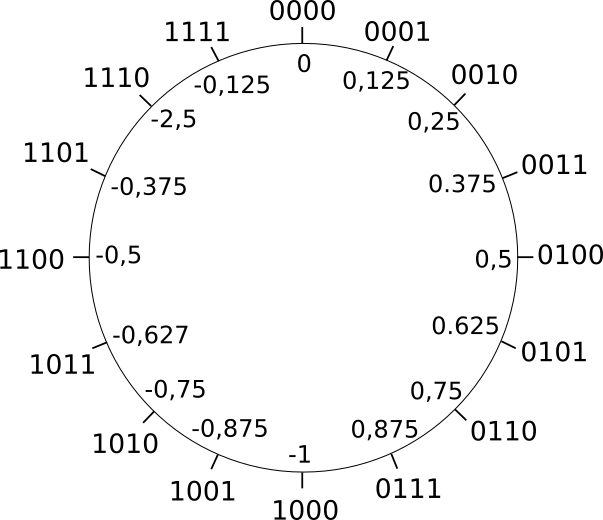
\includegraphics[width=0.5\textwidth]{img/SQ-Kreis.png}
 \caption{Interpretation von Dualzahlen im SQ3-Format.}
 \label{pic:SQKreis}
\end{figure}


Der darstellbare Zahlenbereich liegt hier bei $-1\leq z < 1$. Benötigt werden Zahlen im Bereich von etwa $\pm2$, weshalb ein Vorkommabit benötigt wird. 
Da 12 Bit zur Verfügung stehen, von denen eins für das Vorzeichen und ein weiteres für eine Vorkommastelle verwendet werden, bleiben 10 Bits für die Nachkommazahlen übrig.
Die Aufteilung der Bits wird über die Bezeichnung S1Q10 definiert.
Da für den Quotient 10 Bit zur Verfügung stehen, beträgt die maximale Auflösung $1\,LSB = 2^{-10} = {1024}^{-1} = 9,765625\cdot10^{-4}$.
Der Wertebereich liegt in diesem Fall liegt bei \num{-2} bis \num{1,999023438}. 

Für die Addition oder Multiplikation zweier Zahlen müssen beide einerseits dieselbe Bitbreite und andererseits das gleiche Darstellungsformat besitzen.



 
\subsection{Numerisch bedingte Ungenauigkeiten}\label{sec:NumerischeUngenauigkeiten}
Numerische Ungenauigkeiten entstehen immer dann, wenn die zur Verfügung stehenden Bits es nicht ermöglichen eine Zahl exakt abzubilden. 
Bei einem Bitshift, welcher häufig für die Division durch Zwei oder Vielfachen von Zwei verwendet wird, kann immer Information verloren gehen. Dies ist immer dann der Fall,
wenn die Bits die abgeschnitten werden eine 1 sind. Das hat zur Folge, dass beispielsweise
bei einer Division durch Zwei der resultierende Wert um 1\,LSB kleiner ist, als er eigentlich sein sollte. 
Dieses Problem kann bei jedem Bitshift auftreten. Die Wahrscheinlichkeit für eine 1 liegt im Mittel bei \SI{50}{\percent}, weshalb davon ausgegangen werden muss, dass ein 
positives Ergebnis etwas kleiner und ein negatives vom Betrag her etwas größer ist, als bei verlustfreier Berechnung. 

% Von Prof. Vollmer: 
% \begin{equation}
%  S_N = \frac{P_Q}{\left(2^0\right)^2} + \dfrac{P_Q}{\left(2^1\right)^2} + \dfrac{P_Q}{\left(2^2\right)^2} + \cdots + \dfrac{P_Q}{\left(2^{L-1}\right)^2}
% \end{equation}
% L : Stufe (Additionstakte?)

Da diese Arbeit den Schwerpunkt in der Aufwandsabschätzung einer Chipimplementation einer 2D-DFT auf einem \gls{asic} hat, ist diese Problematik kein Gegenstand dieser Arbeit und
wird an dieser Stelle nur in Grundzügen erwähnt. %Für eine 


 \section{Komplexe Multiplikation}

Im allgemeinen Fall müssen gemäß Gl. \ref{eq:komplexe_Multiplikation} bei der komplexen Multiplikation vier einfache Multiplikation sowie zwei Additionen durchgeführt werden.

\begin{align}\label{eq:komplexe_Multiplikation}
\begin{split}
 e + jf &= (a + jb) \cdot (c + jd)\\
        &= a \cdot c + j(a \cdot d) + j(b \cdot c) + j^2(b \cdot d)\\
        &= a \cdot c + b \cdot d + j(a \cdot d + b \cdot c)
\end{split}
\end{align}



 \section{Matrixmultiplikation}

% Betrachtet wird zunächst die Multiplikation einer Matrix mit einem Vektor.
% 
% \begingroup
% \renewcommand*{\arraystretch}{1.0}
% 
%  \[
%    \begin{bmatrix}
%     \myBlackBox 	& \myBlackBox 		& \myBlackBox 		& \myBlackBox \\
%     \myLightgrayBox 	& \myLightgrayBox 	& \myLightgrayBox 	& \myLightgrayBox \\
%     \myLightgrayBox 	& \myLightgrayBox 	& \myLightgrayBox 	& \myLightgrayBox \\
%     \myLightgrayBox 	& \myLightgrayBox 	& \myLightgrayBox 	& \myLightgrayBox
%    \end{bmatrix}
%   \cdot
%    \begin{bmatrix}
%     \myBlackBox \\
%     \myBlackBox \\
%     \myBlackBox \\
%     \myBlackBox
%    \end{bmatrix}
%   =
%   \begin{bmatrix}%
%    \myBlackBox \\
%    \myLightgrayBox \\
%    \myLightgrayBox \\
%    \myLightgrayBox
%   \end{bmatrix}
%  \]
% \endgroup
% 
%  \vspace{1cm}  
 
 


Um nachfolgende Abschnitte besser erörten zu können, soll zunächst die Matrizenmultiplikation besprochen werden.
Wie in Abbildung \ref{eq:grafikMatrizenmultiplikation} verdeutlicht, wird Element$(i,j)$ der Ergebnismatrix dadurch berechnet, dass die Elemente$(i,k)$ einer Zeile der 1. Matrix
mit den Elementn$(k,j)$ aus der zweiten Matrix multipliziert und die Werte aufsummiert werden. $i$ und $j$ sind für die Berechnung eines Elements konstant, während $k$ über alle
Elemente einer Zeile bzw. Spalte läuft.

\begin{center}
 
\begin{minipage}{0.2\textwidth}
 \begingroup
 \renewcommand*{\arraystretch}{1.1} % Zeilenabstand
 \renewcommand*{\arraycolsep}{0.6pt} % Spaltenabstand

 \[
    \begin{bmatrix}
    \tikzmark{varrowtopleft} \myBlackBox  	& \myBlackBox 		& \myBlackBox 		& \tikzmark{varrowtopright} \myBlackBox \\
                             \myLightgrayBox 	& \myLightgrayBox 	& \myLightgrayBox 	& \myLightgrayBox \\
                             \myLightgrayBox 	& \myLightgrayBox	& \myLightgrayBox	& \myLightgrayBox \\
    \tikzmark{varrowbottom}  \myLightgrayBox 	& \myLightgrayBox 	& \myLightgrayBox 	& \myLightgrayBox 
   \end{bmatrix}
 \]
 \endgroup
  \tikz[overlay,remember picture] {
  \draw[->] ([yshift=1.5ex,xshift=-2ex]varrowtopleft) -- ([xshift=-2ex]varrowbottom)
            node[midway,left] {$i$};
  \draw[->] ([xshift=2ex,yshift=4ex]varrowtopleft) -- ([yshift=4ex]varrowtopright)
            node[midway,above] {$k$};
}
\end{minipage}
\begin{minipage}{0.1\textwidth}
 \hspace{-.5cm}
 \[
  \cdot
 \]
\end{minipage}
\begin{minipage}{0.2\textwidth}
 \begingroup
 \renewcommand*{\arraystretch}{1.1} % Zeilenabstand
 \renewcommand*{\arraycolsep}{0.6pt} % Spaltenabstand
 \[
   \begin{bmatrix}
    \tikzmark{varrowtopleft} \myLightgrayBoxHigh & \myBlackBoxHigh & \myLightgrayBoxHigh & \tikzmark{varrowtopright} \myLightgrayBoxHigh \\
                             \myLightgrayBoxHigh & \myBlackBoxHigh & \myLightgrayBoxHigh & \myLightgrayBoxHigh \\
                             \myLightgrayBoxHigh & \myBlackBoxHigh & \myLightgrayBoxHigh & \myLightgrayBoxHigh \\
    \tikzmark{varrowbottom}  \myLightgrayBoxHigh & \myBlackBoxHigh & \myLightgrayBoxHigh & \myLightgrayBoxHigh 
   \end{bmatrix}
 \]
 \endgroup
   \tikz[overlay,remember picture] {
  \draw[->] ([yshift=1.5ex,xshift=-2ex]varrowtopleft) -- ([xshift=-2ex]varrowbottom)
            node[midway,left] {$k$};
  \draw[->] ([xshift=2ex,yshift=4.5ex]varrowtopleft) -- ([yshift=4.5ex]varrowtopright)
            node[midway,above] {$j$};
}
\end{minipage}
\begin{minipage}{0.05\textwidth}
 \[
  =
 \]
\end{minipage}
\begin{minipage}{0.3\textwidth}
\begingroup
\renewcommand*{\arraystretch}{1.1} % Zeilenabstand
\renewcommand*{\arraycolsep}{0.8pt} % Spaltenabstand
\begin{align}\label{eq:grafikMatrizenmultiplikation}
   \begin{bmatrix}
    \tikzmark{varrowtopleft} \myLightgrayBox 	& \myBlackBox		& \myLightgrayBox 	& \tikzmark{varrowtopright} \myLightgrayBox \\
                             \myLightgrayBox 	& \myLightgrayBox 	& \myLightgrayBox 	& \myLightgrayBox \\
                             \myLightgrayBox 	& \myLightgrayBox 	& \myLightgrayBox 	& \myLightgrayBox \\
    \tikzmark{varrowbottom}  \myLightgrayBox 	& \myLightgrayBox 	& \myLightgrayBox 	& \myLightgrayBox 
   \end{bmatrix}
 \end{align} 
 \endgroup
    \tikz[overlay,remember picture] {
  \draw[->] ([yshift=1.5ex,xshift=-2ex]varrowtopleft) -- ([xshift=-2ex]varrowbottom)
            node[midway,left] {$i$};
  \draw[->] ([xshift=2ex,yshift=4ex]varrowtopleft) -- ([yshift=4ex]varrowtopright)
            node[midway,above] {$j$};
}
\end{minipage}
\end{center}

 \section{Fourierreihenentwicklung}
Mit einer Fourierreihe kann ein periodisches, abschnittsweise stetiges Signal aus einer Summe von Sinus- und Konsinusfunktionen
zusammengesetzt werden. Die Schreibweise als Summe von Sinus- und Kosinusfunktionen (Gl. \ref{eq:Fourierreihenentwicklung}) ist eine 
der häufigsten Darstellungsformen.

\begin{equation}\label{eq:Fourierreihenentwicklung}
 x(t) = \frac{a_0}{2} + \sum_{k=1}^\infty \left(a_k cos(kt) + b_k sin(kt)\right)
\end{equation}

Die Fourierkoeffizienten lassen sich über die Gleichungen (\ref{eq:a_k}) und (\ref{eq:b_k}) berechnen:

\begin{equation}\label{eq:a_k}
 a_k = \frac{1}{\pi} \int_{-\pi}^{\pi} x(t) \cdot cos(kt) dt \quad \textrm{für} \quad k \geq 0 
\end{equation}
\begin{equation}\label{eq:b_k}
 b_k = \frac{1}{\pi} \int_{-\pi}^{\pi} x(t) \cdot sin(kt) dt \quad \textrm{für} \quad k \geq 1
\end{equation}

Mit der Exponentialschreibweise lassen sich Sinus und Kosinus auch wie in (\ref{eq:cos_exp}) und (\ref{eq:sin_exp}) ausdrücken:

\begin{equation}\label{eq:cos_exp}
 cos(k t) = \frac{1}{2}\left(e^{j k t} + e^{-j k t} \right)
\end{equation}

\begin{equation}\label{eq:sin_exp}
 sin(k t) = \frac{1}{2j}\left(e^{j k t} - e^{-j k t} \right)
\end{equation}

und zusammengefasst ergibt sich in (Gl. \ref{eq:komplexerZeiger}) der komplexe Zeiger, der eine Rotation im Gegenuhrzeigersinn auf dem Einheitskreis beschreibt.
In Abbildung \ref{pic:Einheitskreis} dies zusätzlich noch grafisch dargestellt.

 \begin{align}
\begin{split}\label{eq:komplexerZeiger}
cos(k t) +j\cdot sin(k t) &= \frac{1}{2}\left(e^{j k t} + e^{-j k t} \right)+j\cdot \frac{1}{2j}\left(e^{j k t} - e^{-j k t} \right)\\
&= \frac{1}{2} \left(e^{j k t} + e^{j k t}\right)\\
&= e^{j k t}\\
\end{split}
\end{align}


\tikzstyle{dot}=[draw,shape=circle]
\begin{figure}[ht]
\centering
\begin{tikzpicture}[scale=2.5]
\draw[step=.5cm,gray, thin];
\draw (-1.2,0) -> (1.2,0);
\draw (0,-1.2) ->(0,1.2);
\draw (0,0) circle[radius=1cm];
\draw [thick, dashed] (0,0.5) -- (0.866, 0.5);
\draw [thick, dashed] (0.866, 0) -- (0.866, 0.5);
\draw [thick] (0, 0) -- (0.866, 0.5);
\draw (1.1, 0.1) node {1};
\draw (1, 0.6) node {$e^{jkt}$};
\draw (1.1, 0.1) node {1};
\draw (-0.07, 1.1) node {$j$};
\draw (-1.1, 0.1) node {-1};
\draw (-0.15, -1.1) node {$-j$};
\node[dot, fill, inner sep=1pt] at(0.866,0.5){};
\draw [decorate,decoration={gray,brace,amplitude=5pt,raise=2pt},yshift=0pt](0,0) -- (0,0.5) node [rotate=90,black,midway,yshift=0.6cm]{$sin (kt)$};
\draw [decorate,decoration={brace,amplitude=5pt,mirror,raise=2pt},yshift=0pt](0,0) -- (0.866,0) node [black,midway,yshift=-0.6cm]{$cos (kt)$};
\end{tikzpicture}
\caption{Einheitskreis, Zusammensetzung des komplexen Zeigers aus Sinus und Kosinus}
\label{pic:Einheitskreis}
\end{figure}


Die Fourierkoeffizienten $a_k$ und $b_k$ lassen sich auch als komplexe Zahl $c_k$ zusammengefasst berechnen:

\begin{equation}
 c_k = \frac{1}{2\pi} \int_{-\pi}^{\pi} x(t) e^{-j2\pi kt} dt \quad \forall k \in \mathbb{Z}
\end{equation}



\begin{equation}
 x(t) = \sum_{-\infty}^{\infty} c_k e^{jkt}
\end{equation}


\section{Fouriertransformation}
Mit der Fouriertransformation kann ein periodisches, abschnittsweise stetiges Signal $f(x)$ in eine Summe aus Sinus- und
Kosinusfunktionen unterschiedlicher Frequenzen zerlegt werden. Da diese Funktionen jeweils mit nur einer Frequenz periodisch sind, entsprechen diese
Frequenzen den Frequenzbestandteilen von $f(x)$. 

Grundlage für die Fouriertransformation ist das Fourierintegral (Gl. \ref{eq:Fouriertransformation})

\begin{equation}\label{eq:Fouriertransformation}
 X(f) = \int^{\infty}_{-\infty} x(t) \cdot e^{-j 2 \pi f t}
\end{equation}

Wenn Sinus und Kosinus wie in \ref{eq:cos_exp} und \ref{eq:sin_exp} als Exponentialfunktion geschrieben werden,
können sie auch zu einer komplexen Exponentialfunktion zusammengefasst werden.






Für komplexere Signale, etwa ein Rechteck, ergeben sich entsprechend sehr viele dieser Peaks. Deren Höhe ist Information darüber, wie groß ihr Anteil, also die Amplitude des 
Zeitsignals, ist. Die Fouriertransformation kann als das Gegenteil der Fourierreihenentwicklung gesehen werden.


- unendliche Dauer? -> Leistungssignal?

Fourier-Transform: Zerlegung - endliche Dauer, Energiesignal

Energiesignal:
Leistungssignal: Signal unendlicher Energie, aber mit endlicher mittlerer Leistung

Ein Zeitsignal hat ein eindeutig zuordbares Frequenzsignal (bijektiv), abgehsehen von Amplitude? und Phase

Spektrum: Frequenzbestandteile eines Signals
Berechnung des Spektrums: Spektralanalyse, Frequenzanalyse


Fourier-Synthese: Umkehrfunktion

In der Praxis, also basierend auf echten Messdaten, wird die die Bestimmung des Spektrums Spektrumschätzung genannt.


In der vorliegenden Arbeit wird künftig $X^*$ für die 1D-DFT und $X$ für die 2D-DFT stehen.
 \section{Diskrete Fouriertransformation (DFT)}




\subsection{Verwendung}

Die \gls{dft} (Gl. \ref{eq:dft}) ist die zeit- und wertdiskrete Variante der \gls{ft}, die statt von $-\infty$ bis $\infty$ nur von 0 bis N-1 Elemente läuft. 
Im Frequenzspektrum wiederholt sich 
Da es sich um diskrete Werte handelt, geht das Integral in eine endliche Summe über. Die 2D-DFT ist nur möglich (sinnvoll), wenn die Eingangswerte in Form eines Vektors vorliegen.


\subsection{Summen- und Matrizenschreibweise der DFT}
\subsubsection{1D-DFT}
Die \gls{1d-dft} findet wie bereits erwähnt üblicherweise Anwendung, um vom Zeit- in den Frequenzbereich zu gelangen.
\begin{equation}\label{eq:dft}
 X^* \left[ m \right] = \frac{1}{N} \cdot \sum^{N-1}_{n=0} x[n] \cdot e^{-\frac{j 2 \pi m n}{N}}
\end{equation}



Gleichung \ref{eq:1D-DFT_MatrixMult} zeigt die obige Summenformel umgeschrieben zu einer Matrixmultiplikation.

Mit Gleichung \ref{eq:Twiddlefaktorenberechnung} werden zunächst alle Twiddlefaktoren in Matrixform berechnet, wobei n der Index des zu Berechnenden Elements des Vektors im Zeitbereich und
m das Äquivalent im Frequenzbereich ist.
\begin{equation}\label{eq:Twiddlefaktorenberechnung}
\sum^{N-1 }_{m=0} \sum^{N-1 }_{n=0} e^{-\frac{j 2 \pi m n}{N}} = W
\end{equation}


Somit gilt:

\begin{equation}\label{eq:1D-DFT_MatrixMult}
X^* = W \cdot x
\end{equation}

In Matlab kann die Twiddlefaktormatrix mit
\begin{equation}\label{eq:matlab_dft_faktoren}
 W = e^{-\frac{i 2 \pi}{N}\cdot[0:N-1]'\cdot[0:N-1]}
\end{equation}
berechnet werden.


\subsubsection{2D-DFT}
Die \gls{2d-dft} wird hingegen häufig in der Bildverarbeitung verwendet, um vom Orts- in den Fourierraum zu gelagen. Da es sich somit nicht mehr um eine Abhänigkeit 
der Zeit handelt, werden andere Indizes verwendet.
\begin{align}
\begin{split}
X[u,v] 	&= \frac{1}{N} \sum^{N-1}_{n=0} X^* \left[ m \right] \cdot e^{-\frac{j 2 \pi m n}{N}}\\
	&= \frac{1}{MN} \sum^{M-1}_{m=0} \left( \sum^{N-1}_{n=0} f(m,n) \cdot e^{-\frac{j 2 \pi m n}{N}} \right) \cdot e^{-\frac{j 2 \pi m n}{M}}
\end{split}
\end{align}

Auch hier lässt sich die Berechnung in Matrizenschreibweise darstellen:

\begin{align}
\begin{split}
 X &= W \cdot x\left(t\right) \cdot W \\
                    &= X^* \cdot W
\end{split}
\end{align}


\subsection{Rein reelle 2D-DFT}
Bei der oben beschriebenen Berechnung können die Eingangssignale auch komplex sein. Da das Ausgnagssignal der 1D-DFT unabhängig von den Eingangssignalen in jedem Fall 
komplex ist, kann es dort direkt als Eingangssignal für die komplexe 2D-DFT genutzt werden. 
Es wäre jedoch auch möglich, das komplexe Ausgnagssignal der 1D-DFT als zwei von einander unabhängige rein relle Eingangssignale der 2D-DFTs zu betrachten und später 
wieder zusammen zu setzen. Hierbei können aus Symmetriegründen Multiplikationen eingespart werden. Allerdings ist es erforderlich, dass die gespiegelten Werte 
negiert werden.
Interessant ist dieser Ansatz dann, wenn die Recheneinheit so klein wie irgend möglich gehalten werden soll. Zu bedenken gilt es dann, dass zusätzlicher Speicher für 
Zwischenwerte vorhanden sein muss. Da der Platzbedarf hierfür nicht zu unterschätzen ist, relativiert sich die Ersparnis in gewissen Umfang. Auf eine Gegenüberstellung
wird an dieser Stelle verzichtet, die Berechnung als rein relles Signal wird nachfolgend gezeigt.

\begin{equation}
 x = cos(a) + j \cdot sin(b) 
\end{equation}


\begin{equation}
\begin{align}
 X1_{1D} = W \cdot cos(a)\\
 X2_{1D} = W \cdot sin(b)
\end{align}
\end{equation}

% \begin{equation}
% \begin{split}
%  X1_{1D,real} = \Re(X1_{1D}\\
%  X1_{1D,imag} = \Im(X1_{1D}\\
%  X2_{1D,real} = \Re(X2_{1D}\\
%  X2_{1D,imag} = \Im(X2_{1D}
% \end{split}
% \end{equation}
% 
% \begin{equation}
%  \begin{split}
%   X31_{2D} = X1_{1D,real} \cdot W\\
%   X32_{2D} = X1_{1D,imag} \cdot W\\
%   X41_{2D} = X2_{1D,real} \cdot W\\
%   X42_{2D} = X2_{1D,imag} \cdot W
%  \end{split}
% \end{equation}

% \begin{equation}
%  \begin{split}
%   
%  \end{split}
% \end{equation}




Da die gegebenen Eingangssignale aus einer Sinus- und einer Kosinuskomponente bestehen und es sich auf diese Weise als ein komplexes Signal auffassen lässt, kann die 
komplexe Berechnung sowohl bei der 1D-DFT als auch bei der 2D-DFT genutzt werden. 
Da hierdurch in beiden Fällen eine vollständige Auslastung einer komplexen Berechnung gegeben ist und wie bereits erwähnt bei der reellen Berechnung zusätzlicher Speicher 
erforderlich wäre, wird dieses Verfahren angewandt.


\subsection{Inverse DFT}

Die \gls{idft} wird analog zur \gls{dft} mit 

\begin{equation}\label{eq:idft}
 x \left[ n \right] = \frac{1}{N} \sum^{N-1}_{n=0} X[m] \cdot e^{\frac{j 2 \pi m n}{N}}
\end{equation}

beschrieben. Durch die umgekehrte Drehrichtung des komplexen Zeigers werden in der Matrizenschreibweise die Zeilen 1 und 7, 2 und 6 sowie 3 und 5 vertauscht.



 
 \subsection{Berechnung der schnellen Fouriertransformation}\label{sec:BerechnungFFT}
Die Mathematiker Cooley und Tukey haben einen Algorithmus entwickelt und im Jahr 1965 veröffentlicht, mit dem sich die \gls{dft} mit weniger Multiplikationen
und dadurch schneller als bei der allgemeinen \gls{dft} berechnen lässt. Das Verfahren wird als \gls{fft} bezeichnet.
Grundlage ist, dass sich eine DFT
in kleinere Teil-DFTs aufspalten lässt, welche durch Ausnutzen von Symmetrieeigenschaften in der Summe weniger Koeffizienten haben. 
Üblich ist die Radix-2 FFT, Ausgangspunkt ist eine DFT mit 2 Eingangswerten. 
Diese Methode kann nur auf Eingangsvektoren der Größe $2^n$ angewandt werden. Dieser
vermeintliche Nachteil lässt sich durch Auffüllen des Eingangsvektors mit Nullen (Zeropadding) eliminieren. Dies hat zur Folge, dass die Größe des Ausgangsvektors
immer eine Potenz von zwei ist. 
Die Anzahl der benötigten komplexen Multiplikationen $m_{FFT}$ kann mit der Gleichung (\ref{eq:FFT_komplexMult}) abgeschätzt werden.


\begin{equation}\label{eq:FFT_komplexMult}
 m_{FFT} = \frac{N}{2}\log_2(N)
\end{equation}



Das Verfahren wird in Kürze in Kapitel \ref{sec:AnalyseFFT} behandelt und kann unter anderem in dem Buch 
\textit{Digital Signal Processing: Principles, Algorithms and Applications}~\autocite{john2007digital} auf den Seiten 511 bis 524 nachgelesen werden.
 \subsection{Inverse DFT}

Die \gls{idft} ist die Umkehrfunktion der \gls{dft}. Wenn das Eingangssignal $x[n]$ zeitabhängig und somit als $\vec{x}(t)$ geschrieben werden kann, dann handelt es sich bei $X^*[m]$ um
dessen Darstellung im Frequenzbereich und kann als $\vec{X^*}(f)$ geschrieben werden. Mit der \gls{idft} ist es möglich, aus der Frequenzdarstellung das Zeitsignal zu errechnen.
%$X(f)$ $x(t)$ 

\begin{equation}\label{eq:idft}
 x \left[ n \right] = \frac{1}{N} \sum^{N-1}_{n=0} X^*[m] \cdot e^{\frac{j 2 \pi m n}{N}}
\end{equation}

beschrieben. Gleichung (\ref{eq:idft}) ist bis auf die Drehrichtung des komplexen Zeigers und die Vertauschten Ein- und Ausgangsvektoren identisch zu Gleichung (\ref{eq:dft}).
 \section{Diskrete Kosinus Transformation (DCT)}
\subsection{Verwendung}


\subsection{Berechnung}
Für die Berechnung der DCT gibt es verschiedene Varianten, welche sich in der Symmetrie der Ergebnismatrix unterscheiden. (Stimmt das wirklich? was sonst?)

Darüber hinaus wird in der Bildverarbeitung häufig die 1. Zeile der Twiddlefaktormatrix mit dem Faktor $\frac{1}{\sqrt2}$, sowie die gesamte Matrix mit 
$\sqrt{\frac{2}{N}}$, $N =$ Anzahl Elemente in einer Zeile bzw. Spalte, multipliziert.

Da es hier um eine Aufwandsabschätzung geht, wird sich auf die in der Bildverarbeitung gängigste Variante jedoch ohne die skalierenden Faktoren beschränkt.
Diese berechnet sich zu

\begin{equation}
X_k = \sum_{n=0}^{N-1} x_n \cos\left[\frac{\pi k}{N} \left(n+\frac{1}{2}\right) \right] \quad \textrm{für} \quad  k=0,\dots,N-1
\end{equation}

Die Twiddlefaktormatrix kann in Matlab mit
 %\lstinputlisting[language=matlab, caption={}, frame=no, numbers=none, label=src:dct_faktoren]{Skripte/Matlab/DCT_Faktoren.m}
 \begin{equation}\label{eq:matlab_dct_faktoren}
  W = \cos\left(\frac{\pi}{N}\cdot \left([0:N-1]')*([0:N-1]+\frac{1}{2}\right)\right)
 \end{equation}

berechnet werden. 
 
 
 
 
 
 
 \chapter{Analyse}
 
 \section{Bewertung verschiedener DFT- und DCT-Größen}
In diesem Abschnitt sollen Erkenntnisse gewonnen werden, auf denen basierend später die Wahl der Größe der Transformationsmatrix getroffen werden kann.
\subsection{Bewertung verschiedener DCT-Größen}
In Tabelle \ref{tab:DCT-TwiddlefaktorMatrizenBewertung} ist die Gegenüberstellung der genannten Größen zu sehen. Für die Bewertung wurd das 
Matlab-Skript aus Anhang \ref{src:dct_bewertung} geschrieben.
Ersichtlich ist, dass die Anzahl verschiedener nicht trivialer Werte etwa der Wurzel aus der Anzahl aller Werte ist.
Dies bedeutet im Umkehrschluss, dass im Schnitt jede Zeile einen neuen Faktor einführt. Die Summe nicht trivialer Werte weist bei allen Matrizen
mehr als 50$\%$ auf. 

\begingroup
  \renewcommand*{\arraystretch}{1.2} % Zeilenabstand der Tabelle
\begin{table}[ht!]
 \centering
 \caption{Bewertung der DCT-Twiddlefaktor-Matrizen}
 \begin{tabular}{lccccc}
   \hline  
   N                                                 & 8     & 9      & 12     & 15    & 16\\
   \hline
   N$\times$N                                        & 64    & 81     & 144    & 225   & 256\\
   \rowcolor{lightgray}
   $\sum$ trivialer Werte                            & 8     & 33     & 28     & 63    & 16\\
   \rowcolor{lightgray}
   $\sum$ nicht trivialer Werte                      & 56    & 48     & 116    & 162   & 240\\
   Anzahl verschiedener nicht trivialer Werte        & 7     & 7      & 10     & 13    & 15\\
   Verhältnis $\sum$ trivial / $\sum$ nicht trivial  & 0.143 & 0.6875 & 0.2414 & 0.389 & 0.067\\
   \hline
 \end{tabular}
 \label{tab:DCT-TwiddlefaktorMatrizenBewertung}  
\end{table}
\endgroup

 \subsection{Bewertung verschiedener DFT-Größen}\label{sec:AnalyseBewertungTwiddlefaktornMatrizen}

In der Tabelle \ref{tab:DFT-TwiddlefaktorMatrizenBewertung} werden die DFT-Matrizen einander gegenüber gestellt.
Anders als die \gls{dct} haben die Twiddlefaktormatrix und deshalb auch das Ergebnis der \gls{dft} einen Real- und einen Imaginärteil.
Die Beurteilung basiert auf dem Matlab-Skript aus Anhang \ref{src:dft_bewertung}. 
Wie zu sehen ist, schneiden vor allem die 8x8- und die 12x12-DFT gut ab. Da letztere nur zum Vergleich mit aufgenommen wurde, ist die 
8x8-DFT der klare Favorit, welcher im folgenden Abschnitt genauer betrachtet werden soll.


 \vspace{1cm}
 \begingroup
  \renewcommand*{\arraystretch}{1.2} % Zeilenabstand der Tabelle
  \begin{table}[!ht]
  \centering
  \caption{Bewertung der DFT-Twiddlefaktor-Matrizen}
   \begin{tabular}{lccccc}
   \hline
    N							& 8	& 9	& 12	& 15		& 16 \\
    \hline
    N$\times$N						& 64	& 81	& 144	& 225		& 256 \\
    \rowcolor{lightgray}
    trivial $\Re$ 					& 48	& 45	& 128	& 81		& 128 \\
    \rowcolor{lightgray}
    nicht triv. $\Re$					& 16	& 36	& 16	& 144		& 128 \\
    triv. $\Im$ 					& 48	& 21	& 96	& 45		& 128 \\
    nicht triv. $\Im$ 					& 16	& 60	& 48	& 180		& 128 \\
    \rowcolor{lightgray}
    $\sum$ triv. 					& 96	& 66	& 224	& 126		& 256 \\
    \rowcolor{lightgray}
    $\sum$ nicht triv. 					& 32	& 96	& 64	& 324		& 256 \\
    Anzahl verschiedener nicht trivialer Werte          & 1     & 7     & 1     & 13            & 3 \\
    Verhältnis  $\sum$ trivial / $\sum$ nicht trivial	& 3	& 0,6875& 3,5	& 0,3889	& 1\\
    \hline
   \end{tabular}
   \label{tab:DFT-TwiddlefaktorMatrizenBewertung}
  \end{table}
 \endgroup
 \vspace{1cm}
 
 
 \subsection{Bewertungsfazit}
 Sowohl die \gls{dct} als auch die \gls{dft} finden häufig in der Bildverarbeitung Anwendung, so dass bereits diverse Algorithmen für die weiteren
 Berechnungen vorhanden sind. Beide haben symmetrische Twiddlefaktormatrizen.
 Der Vorteil der \gls{dct} gegenüber der \gls{dft} ist, dass sie rein reelle Ergebniswerte liefert. 
 Dem steht als großer Nachteil gegenüber, dass beinahe alle ihrer Twiddlefaktoren zu den nicht trivialen gezählt werden müssen. 
 Des Weiteren verteilen sich ihre Werte auf mehr verschiedene Zahlen, sodass eine effiziente Implementierung gegenüber der DFT, trotz der rein reellen
 Werte, weniger praktikabel erscheint.
 
 Als Ausschlag gebendes Kriterium wird letztlich der Vorteil eines komplexen Ergebnisses herangezogen, aus dem sich ohne Umwege der Winkel berechnen lässt.

 

 
 
 \section{Genauere Betrachtung der 8x8-DFT}\label{sec:AnalyseGenauereBetrachtung8x8}
 Da die 8x8-DFT als Favorit aus der Betrachtung der Transformationsmatrizen herausgegangen ist, wird diese im nächsten Abschnitt auf ihre Eigenschaften
 hin untersucht. Dies wird die Grundlage für eine effiziente Implementierung sein. 
 Die Twiddlefaktormatrix der 8x8-DFT besteht, wie bereits aus Gleichung (\ref{eq:Twiddlefaktorenberechnung}) bekannt, aus komplexen Zeigern.
 Die möglichen Werte sind in Abbildung \ref{pic:Einheitskreis_Faktoren} zu sehen, 
 in Abbildung \ref{pic:Twiddlefaktoren_Darstellung8x8} sind zur besseren Veranschaulichung die Zeiger auf 8 Einheitskreise aufgeteilt,
 wobei jeder einen Laufindex ($m$) des Zeitbereichs abdeckt. In den einzelnen Kreisen sind wiederum alle Laufindizes ($n$) des Frequenzbereichs zu sehen.
 
  \begin{figure}[!h]
  \centering
  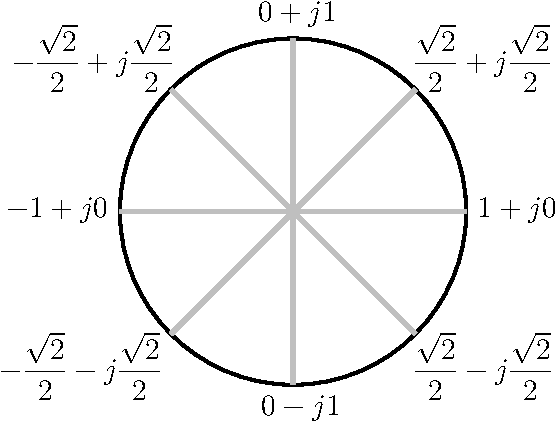
\includegraphics[width=0.4\textwidth]{img/Einheitskreis-crop.pdf}
  \caption{Einheitskreis mit relevanten Werten der 8x8-DFT}
  \label{pic:Einheitskreis_Faktoren}
\end{figure}
  
 


\begin{figure}[!ht]
 \centering
 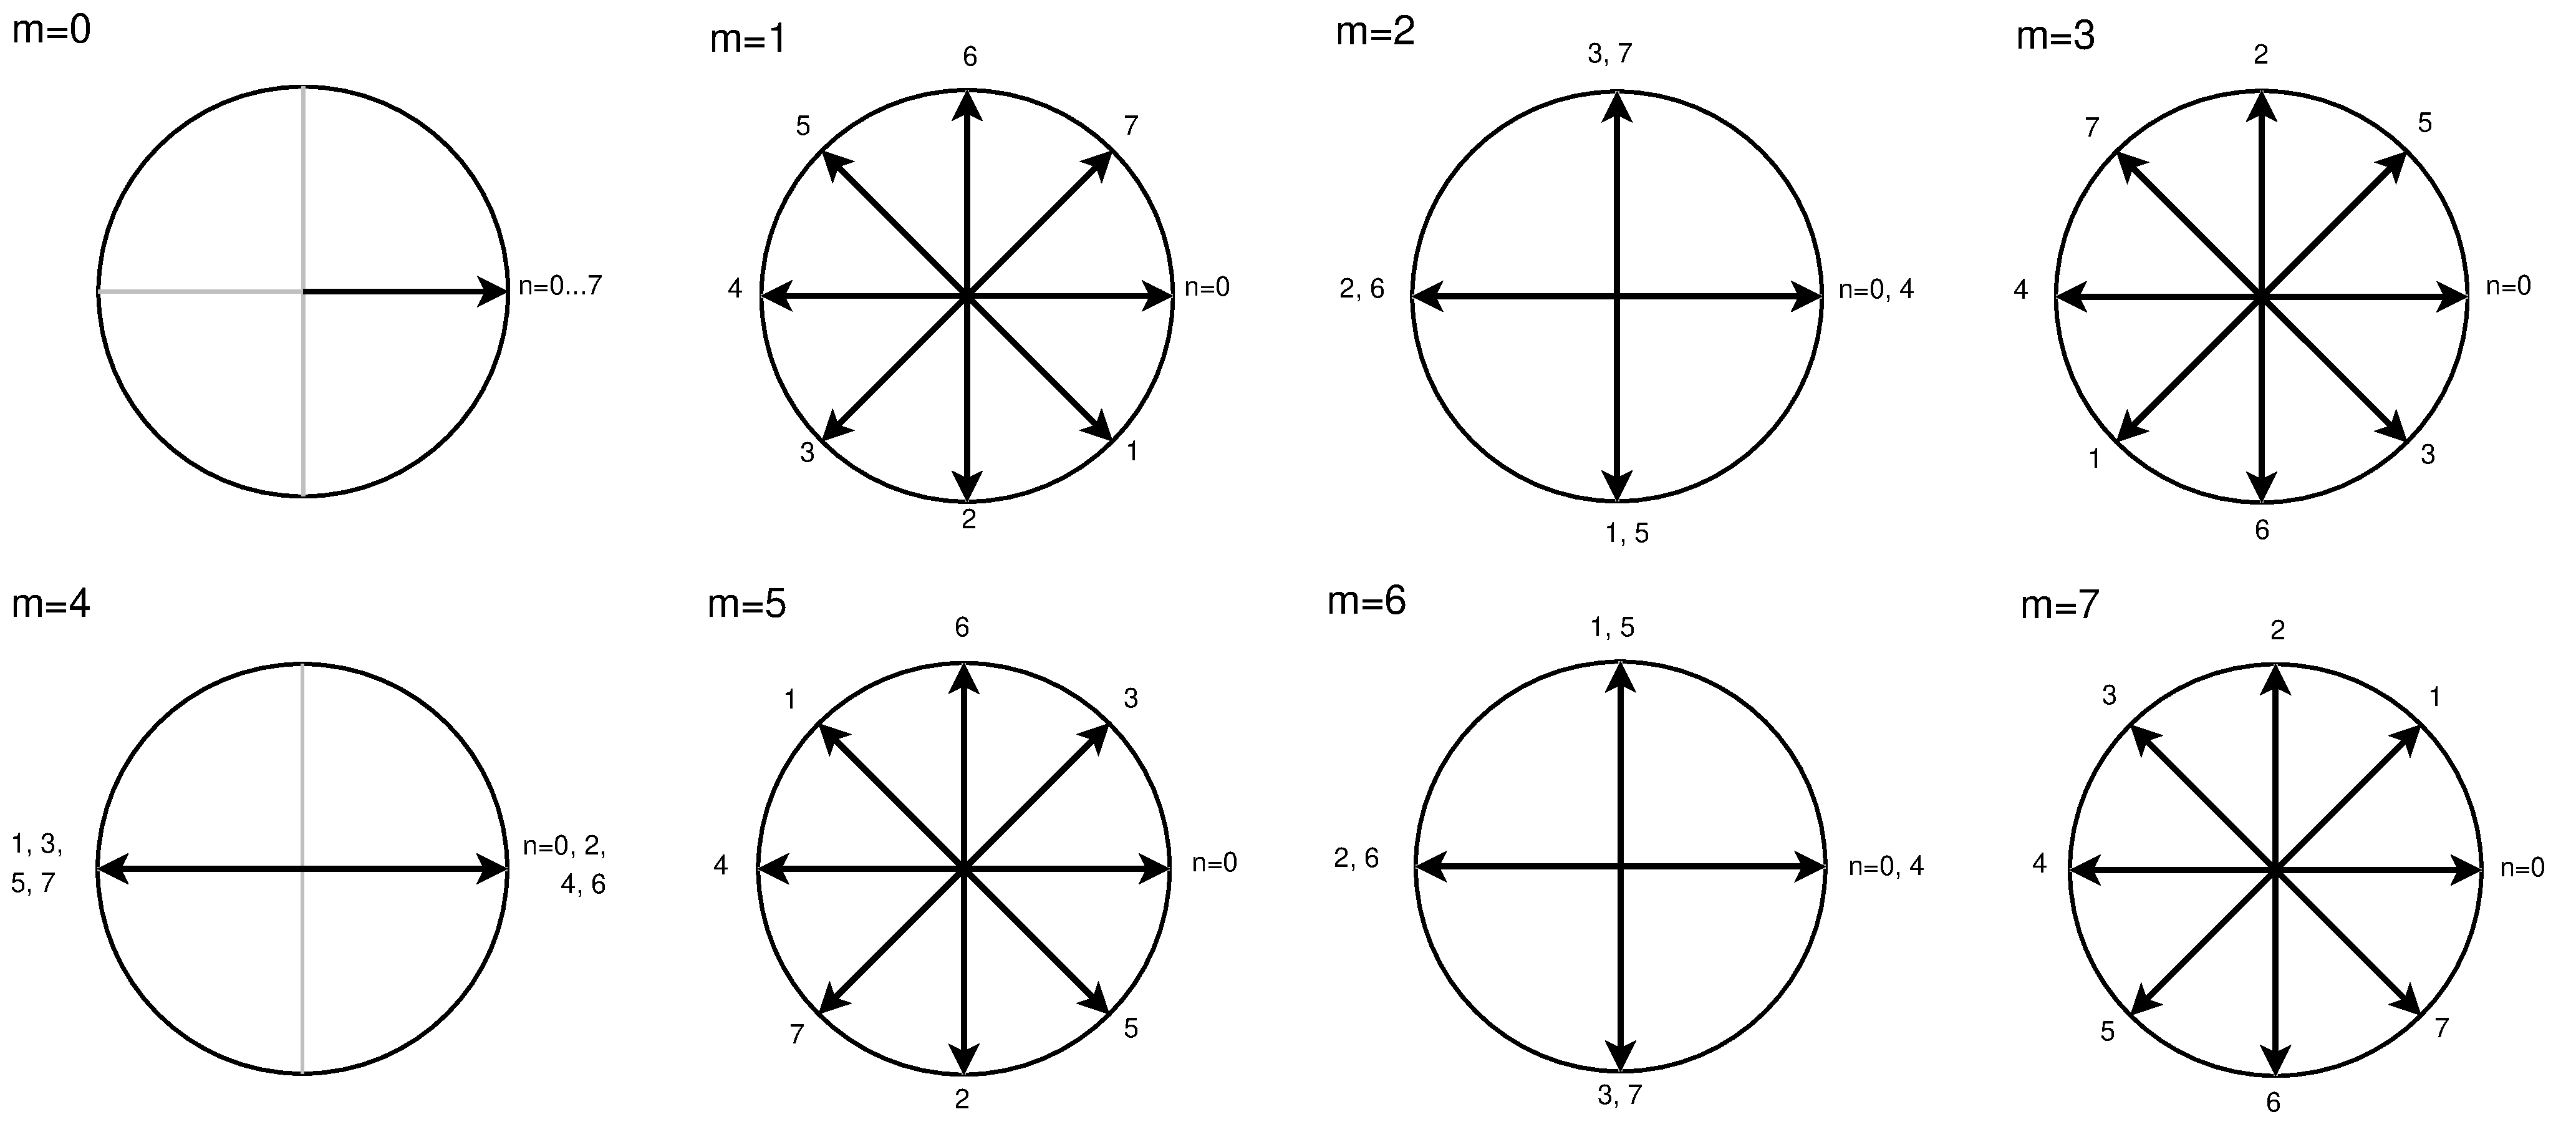
\includegraphics[width=1\textwidth]{img/Twiddlefaktoren_Einheitskreis.eps}
 \caption{Twiddlefaktoren der 8$\times$8-Matrix, aufgeteilt auf die Laufindizes $m$ und $n$. $m$ bezieht sich auf das Element im Ausgangsvektor $\vec{X}$, $n$ auf den Eingangsvektor $\vec{x}$. Siehe auch Gl. (\ref{eq:dft}).}
 \label{pic:Twiddlefaktoren_Darstellung8x8}
\end{figure}

\vspace{0.5cm}
 
 Wie anhand der Grafiken \ref{pic:Einheitskreis_Faktoren} zu sehen ist, setzen sich die Faktoren ausschließlich aus den Zahlen $\pm1$, $\pm\nicefrac{\sqrt{2}}{2}$ und $0$ 
 zusammen. Gemäß der Definition für nicht triviale Werte aus Abschnitt \ref{sec:BewertungVerschiedenerGroessen} zählt ausschließlich der letztgenannte zu diesen.
 Ebenfalls ist ersichtlich, dass der Betrag aller Zahlen immer $1$ ist.
 In Abbildung \ref{pic:MatrizenDarstellungTwiddlefaktoren} ist die Twiddlefaktormatrix auf zwei Matrizen aufgeteilt, wobei die Zahlen durch Farben repräsentiert werden.
 Die linke enthält alle realen Anteile, die rechte alle imaginären. 
 Anhand der Grafik lässt sich gut die Symmetrie erkennen, mit der die Werte auftreten. Diese Grafik soll als 
 Ausgangspunkt für die folgende Betrachtung dienen.
 Es lässt sich auch gut erkennen, das die Kreise aus Abbildung \ref{pic:Twiddlefaktoren_Darstellung8x8} die Werte der korrespondierenden Zeilen wiederspiegeln.
 
 \begin{minipage}{0.9\textwidth}
\begingroup
 \renewcommand*{\arraystretch}{0.95} % Zeilenabstand der Tabelle

\begin{center}
  \[
   \stackrel{\mbox{$Re\{W\}$}}{
    \begin{bmatrix}
     \myboxOnePos 	& \myboxOnePos 		& \myboxOnePos 	& \myboxOnePos 		& \myboxOnePos 	& \myboxOnePos 		& \myboxOnePos 	& \myboxOnePos \\
     \myboxOnePos 	& \myboxSqrtPos 	& \myboxZero 	& \myboxSqrtNeg		& \myboxOneNeg	& \myboxSqrtNeg		& \myboxZero	& \myboxSqrtPos \\
     \myboxOnePos 	& \myboxZero 		& \myboxOneNeg 	& \myboxZero 		& \myboxOnePos 	& \myboxZero 		& \myboxOneNeg 	& \myboxZero \\
     \myboxOnePos 	& \myboxSqrtNeg 	& \myboxZero 	& \myboxSqrtPos 	& \myboxOneNeg 	& \myboxSqrtPos 	& \myboxZero 	& \myboxSqrtNeg \\
     \myboxOnePos 	& \myboxOneNeg 		& \myboxOnePos 	& \myboxOneNeg 		& \myboxOnePos 	& \myboxOneNeg 		& \myboxOnePos 	& \myboxOneNeg \\
     \myboxOnePos 	& \myboxSqrtNeg 	& \myboxZero 	& \myboxSqrtPos 	& \myboxOneNeg 	& \myboxSqrtPos 	& \myboxZero 	& \myboxSqrtNeg \\
     \myboxOnePos 	& \myboxZero 		& \myboxOneNeg 	& \myboxZero 		& \myboxOnePos 	& \myboxZero 		& \myboxOneNeg 	& \myboxZero \\
     \myboxOnePos 	& \myboxSqrtPos 	& \myboxZero 	& \myboxSqrtNeg		& \myboxOneNeg	& \myboxSqrtNeg		& \myboxZero	& \myboxSqrtPos 
    \end{bmatrix}
   }
   \hspace{1cm}
   \stackrel{\mbox{$Im\{W\}$}}{
    \begin{bmatrix}
     \myboxZero 	& \myboxZero 		& \myboxZero 	& \myboxZero 		& \myboxZero 	& \myboxZero 		& \myboxZero 	& \myboxZero \\
     \myboxZero 	& \myboxSqrtNeg 	& \myboxOneNeg 	& \myboxSqrtNeg		& \myboxZero	& \myboxSqrtPos		& \myboxOnePos	& \myboxSqrtPos \\
     \myboxZero 	& \myboxOneNeg 		& \myboxZero 	& \myboxOnePos 		& \myboxZero 	& \myboxOneNeg 		& \myboxZero 	& \myboxOnePos \\
     \myboxZero 	& \myboxSqrtNeg 	& \myboxOnePos 	& \myboxSqrtNeg 	& \myboxZero 	& \myboxSqrtPos 	& \myboxOneNeg 	& \myboxSqrtPos \\
     \myboxZero 	& \myboxZero 		& \myboxZero 	& \myboxZero 		& \myboxZero 	& \myboxZero 		& \myboxZero 	& \myboxZero \\
     \myboxZero 	& \myboxSqrtPos 	& \myboxOneNeg 	& \myboxSqrtPos		& \myboxZero 	& \myboxSqrtNeg 	& \myboxOnePos 	& \myboxSqrtNeg \\
     \myboxZero 	& \myboxOnePos 		& \myboxZero 	& \myboxOneNeg 		& \myboxZero 	& \myboxOnePos 		& \myboxZero 	& \myboxOneNeg \\
     \myboxZero 	& \myboxSqrtPos 	& \myboxOnePos 	& \myboxSqrtPos		& \myboxZero	& \myboxSqrtNeg		& \myboxOneNeg	& \myboxSqrtNeg 
    \end{bmatrix}
   }
  \]
\vspace{0.5cm}
  Legende: $\myboxOnePos$ = 1 \quad $\myboxOneNeg$ = -1 \quad $\myboxZero$ = 0 \quad $\myboxSqrtPos$ = $\nicefrac{\sqrt{2}}{2}$ \quad $\myboxSqrtNeg$ = -$\nicefrac{\sqrt{2}}{2}$
  \captionof{figure}{Matrix-Darstellung der 8x8-DFT-Twiddlefaktoren aufgeteilt nach Real- und Imaginärteil.}
  \label{pic:MatrizenDarstellungTwiddlefaktoren}
\end{center}
\endgroup
\end{minipage}


\vspace{0.5cm}
 
 Auf den ersten Blick sticht die erste Zeile hervor, da sie im Realteil nur aus positiven Einsen und im Imaginärteil nur aus Nullen besteht.
 Mit der fünften Zeile verhält es sich ähnlich. Anders ist hier, dass sich positive und negative Einsen abwechseln.
 In die gleiche Gruppe können noch die dritte und die siebte Zeile zusammengefasst werden. 
 %Beide haben gemeinsam, dass sie so wie die erste und fünfte nur Einsen und Nullen als Faktoren haben. 
 Im Unterschied zu den vorigen können hier aber auch die Imaginärteile eine positive bzw. negative Eins haben. Entsprechend ist dann der Realteil
 Null. Hier müssen zur Berechnung des Ergebnisses also auch Imaginärteile der Eingangsmatrix mit einbezogen werden.
 Für die vier bisher betrachteten Zeilen gilt, dass zur Berechnung eines Elements der Ergebnismatrix ausschließlich Additionen oder Subtraktionen erforderlich sind. 
 
 
 Alle Werte, die bis jetzt vorkamen, haben entweder nur einem Real- oder einem Imaginärteil. 
 Dies hat den Vorteil, dass weniger Berechnungen erfolgen müssen, da von einer vollständig komplexen Multiplikation nur eine Multiplikation einer komplexen Zahl mit einer
 rein reellen (bzw. imaginären) übrig bleiben. Auf diese Weise reduziert sich der in Gleichung (\ref{eq:komplexe_Multiplikation}) gezeigte Aufwand zu dem in Gleichung (\ref{eq:halb_komplexe_Multiplikation}).
 Darüber hinaus sind bei den bisherigen Zahlen keine Multiplikationen nötig, weshalb sich der Rechenaufwandt auf den Additionsteil der Gleichung beschränkt.
 
 \begin{align}\label{eq:halb_komplexe_Multiplikation}
 \begin{split}
  e + jf &= a \cdot (c + jd)\\
         &= a \cdot c + j(a \cdot d)\\
 \end{split}
 \end{align}
 
 Für die übrigen vier Zeilen gelten die bisherigen Beobachtungen nicht oder nur teilweise, weshalb sie nicht zur ersten Gruppe gezählt werden können.
 Dafür haben sie aber alle gemein, dass die Hälfte der Faktoren sowohl einen Real- als auch einen Imaginärteil besitzen, welche symmetrisch angeordnet sind.
 Für diese vier Faktoren sind deshalb jeweils die gesamten vier Multiplikationen aus Gleichung \ref{eq:komplexe_Multiplikation} nötig.

 Eine besondere Eigenschaft ist, dass der Faktor für nicht triviale Multiplikationen im Real- und Imaginärteil zumindest vom Betrag her identisch sind.
 Dies liegt daran, dass der Einheitskreis in acht Teile geteilt wird und für beispielsweise $\frac{2\cdot\pi}{8}=\frac{\pi}{4}$ der Sinus- und Kosinuswert identisch sind. 
 Hieraus resultiert, dass die Hälfte der Berechnungen der nicht trivialen Werte, die für die reelle Matrix gemacht werden müssen,
 direkt für den imaginären Anteil übernommen werden könnten. Die andere Hälfte müsste lediglich negiert werden. 
 Deshalb kann das berechnete Verhältnis von 3 in Tabelle \ref{tab:DFT-TwiddlefaktorMatrizenBewertung} als deutlich höher angenommen werden.
 



  \section{Entscheidung DCT vs. DFT}
 Noch nicht fertig!
 
 Sowohl die \gls{dct} als auch die \gls{dft} finden häufig in der Bildverarbeitung Anwendung. Der Vorteil der \gls{dct} gegenüber der \gls{dft} ist,
 dass sie rein reelle Ergebniswerte liefert. Ihr großer Nachteil zeigt sich u.a. insbesondere deutlich bei den 8x8-Matrizen, da sich hier 
 
 
 nicht trivial darstellbare Zahlen der DCT einem einzigen bei der 8x8-DFT gegenüber stehen.
 

Auch wenn bei der DFT mit der Berechnung des imaginären Teils zusätzlicher Implementierungsaufwamd hinzukommt, wird davon ausgegangen, dass dieser geringer ist, 
 als alle x Multiplikationen umzusetzen. Ebenso ist die Annahme, dass der Platzbedarf auf einem Chip in einer ähnlichen Größenordnung liegt, da auf der einen Seite
 der zusätzliche Speicherbedarf für eine weitere Matrix den x Konstantenmultiplizierer-Schaltnetzen gegenüber stehen.
 
 Es ist nicht geklärt, welche Berechnung für eine Weiterverarbeitung sinnvoller ist. Dies heraus zu finden ist jedoch nicht Bestandteil der Aufgabenstellung dieser Arbeit.
 An dieser Stelle sollen lediglich Vor- und Nachteile zusammengetragen werden, die eine Entscheidung rechtfertigen.
 
 Ein Einsatzszenario der Transformationen ist die Filterung von Rauschen und anderen Störgrößen. Hierfür ist die DFT gut geeignet. 
 
 
 Da es bei dieser Arbeit vor allem um die Aufwandsabschätzung einer optimierten Matrizenmultiplikation zur Vorverarbeitung der Sensordaten geht, 
 welche als Ausgangspunkt für eine finale Implementation dient, und es sich hier um keine endgültige Entscheidung handelt, ist die DFT gut geeignet.
 
 
 \begin{table}[ht]
 \centering
  \caption{Gegenüberstellung der Vor- und Nachteile von DCT und DFT}
  \begin{tabular}{lcc}
  \hline
      Eigenschaft          & Vorteil   & Nachteil\\
  \hline
   Imaginärteil Vorhanden  & DCT       & DFT \\
   Anzahl Multiplikationen & DFT       & DCT\\
   Platzbedarf             &  -        &  - \\
   \hline
  \end{tabular}
  \label{tab:gegenüberstellung_dct_dft}
 \end{table}

 
 \section{Abschätzung des Rechenaufwands}\label{sec:abschaetzung_Rechenaufwand}

\subsection{Gegenüberstellung von reellen und komplexen Eingangswerten}\label{sec:GegenüberstellungRelleKomplexeEingangswerte}
Die Sensormatrix liefert für jedes Sensorelement einen Sinus- und einen Kosinuswert. Diese können für die Berechnung der DFT zu einer komplexen Zahl zusammengefasst werden. 
Auf diese Weise lässt sich die Berechnung mathematisch kompakter schreiben.


In Tabelle (\ref{tab:TakteKomplexeDFT}) ist eine Auflistung der für die Berechnung veranschlagten Takte für die Multiplikation einer beliebigen Matrix mit der
Twiddlefaktormatrix für die 8x8-DFT zu sehen. Grundlage ist, dass in einem Takt Summanden 
paarweise aufaddiert werden und in einer Variablen zwischengespeichert werden. Dieses Verfahren kann auch als Baumstruktur aufgefasst werden. 
Wie das Ausummieren erfolgt, kann in Abschnitt (\ref{sec:Berechnungsschema}) detaillierter nachgelesen werden.

Wie in Abschnitt (\ref{sec:Konstantenmultiplizierer}) gezeigt wird, kann die Multiplikation mit einer Konstanten innerhalb eines Taktes mit einem Schaltnetz erfolgen. 
Anders als bei der komplexen Multiplikation mit der Twiddlefaktormatrix sind bei der getrennten Berechnung ungleich viele positive und negative Faktoren je Zeile vorhanden, 
sodass zu diesem Zeitpunkt davon ausgegangen werden muss, dass eine Negation mancher Werte erforderlich sein wird. Um keine zu langen Signal- und Gatterlaufzeiten hervor zu 
rufen, sollte hierfür ebenfalls ein Takt eingeplant werden, wordurch der zeitliche Gewinn wiederum etwas relativiert wird.


\begin{table}[htbp]
\centering
\caption{Takte für die komplexe DFT}
\label{tab:TakteKomplexeDFT}
\begin{tabular}{ccccc}
\hline
\multirow{2}{*}{Zeile} & Additionen & Takte pro Element & Takte für & Summe der\\
      & pro Element ($N$) & ($\log_2(N)$) & Multiplikation & Takte\\
\hline
 1& 8  & 3   &0 &3\\
 2& 12 & 3,6 &1 &5\\
 3& 8  & 3   &0 &3\\
 4& 12 & 3,6 &1 &5\\
 5& 8  & 3   &0 &3\\
 6& 12 & 3,6 &1 &5\\
 7& 8  & 3   &0 &3\\
 8& 12 & 3,6 &1 &5\\
\hline
\end{tabular}
\end{table}

Anhand der rechten Spalte ergeben sich so (3+5)$\cdot$4$\cdot$8 = 256 Takte sowohl für den Real- als auch den Imaginärteil der komplexen Ausgangsmatrix. Real- und Imaginärteil
werden parallel berechnet und sind somit zeitgleich fertig.

Wie ein Vergleich der Gleichungen (\ref{eq:komplexe_Multiplikation}) und (\ref{eq:halb_komplexe_Multiplikation}) zeigt, entfallen die Hälfte der Multiplikationen, wenn die
Eingangswerte in Real- und Imaginärteil getrennt werden.
Wenn die Eingangswerte rein reell sind, kommen beispielsweise keine $j^2$-Komponenten zustande, welche auf die reellen Elemente aufaddiert werden müssten.
Aus diesem Grund müssen weniger Werte aufsummiert werden, wie sich in Tabelle (\ref{tab:TakteReelleDFT}) zeigt.

\begin{align}\label{eq:halb_komplexe_Multiplikation}
\begin{split}
 e + jf &= a \cdot (c + jd)\\
        &= a \cdot c + j(a \cdot d)\\
\end{split}
\end{align}

\begin{table}[htbp]
\centering
\caption{Takte für die reelle DFT am Beispiel der reellen Ausgangsmatrix}
\label{tab:TakteReelleDFT}
\begin{tabular}{ccccc}
\hline
\multirow{2}{*}{Zeile} & Additionen & Takte pro Element & Takte für & Summe der\\
      & pro Element ($N$) & ($\log_2(N)$) & Multiplikation & Takte\\
\hline
 1& 8 & 3   &0 &3\\
 2& 6 & 2,6 &1 &4\\
 3& 4 & 2   &0 &2\\
 4& 6 & 2,6 &1 &4\\
 5& 8 & 3   &0 &3\\
 \rowcolor{lightgray} 6& 6 & 2,6 &1 &4\\
 \rowcolor{lightgray} 7& 4 & 2   &0 &2\\
 \rowcolor{lightgray} 8& 6 & 2,6 &1 &4\\
\hline
\end{tabular}
\end{table}

Aus Abschnitt (\ref{sec:rein_reelle_dft}) ist bekannt, dass die letzten drei Zeilen direkt oder negiert aus den Zeilen 2-4 übernommen werden können. Die Takte der 6.-8. Zeilen
sind deshalb in der Tabelle (\ref{tab:TakteReelleDFT}) grau hinterlegt. Gegenüber der komplexen Matrix ergeben sich hier statt 256 Takten (3+4+2+4+3)$\cdot$8 = 128 Takte. 
Der Imaginärteil errechnet 
sich noch schneller, da die 1. und 5. Zeile keinen Beitrag leisten und auch hier die Zeilen 2-4 in diesem Fall nach einer Negation die Werte der letzten 3 Zeilen ergeben. 
So ergeben sich dort (3+2+3)$\cdot$8=64 Takte. Vermultich müssen an dieser Stelle wieder Takte für das Negieren eingeplant werden. Da beide parallel berechnet werden, sind die 
hierfür benötigten Takte sozusagen frei verfügbar.

Interessant ist dieser Ansatz dann, wenn einerseits die Recheneinheit so klein wie irgend möglich gehalten werden soll und andererseits die Berechnung noch schneller erfolgen muss.
Abbildung (\ref{pic:reelleDFT}) zeigt, dass im Vergleich zur komplexen Berechnung der 2D-DFT voraussichtlich 3x so viel Speicher für Zwischenwerte vorhanden sein muss.
Ingesamt übersteigt so der Flächenbedarf der gesamten Einheit der der komplexen Variante. Auch die Leitungen um den Speicher anzubinden dürfen nicht vernachlässigt werden.

 
\subsection{Direkte Multiplikation zweier 8x8 Matrizen}
Die in Abschnitt (\ref{sec:Matrixmultiplikation}) erläuterte Matrixmultiplikation bedarf bei einer 8x8 Matrix je Ergebnis der Ausgangsmatrix 8 Multiplikationen. Für
die 8$\cdot$8=64 Elemente werden deshalb 512 Multiplikationen benötigt. Da es sich sowohl bei den Eingangswerten als auch bei der Twiddlefaktormatrix um komplexe
Zahlen handelt, sind, wie in Abschnitt (\ref{sec:komplexe_Multiplikation}) beschrieben, insgesamt 512$\cdot$4=2048 Multiplikationen nötig.

Sollte sich dazu entschieden werden die Sinus- und Kosinusanteile separat zu berechnen, um ein rein reelles Eingangssignal weiter zu verarbeiten, sind, wie in Abschnitt
(\ref{sec:rein_reelle_dft}) hergeleitet, knapp die Hälfte der Multiplikationen unnötig. In Abbildung (\ref{pic:reelleMatMultRedundanz}) ist zu sehen, dass von den 64 
Ergebniswerten nur 40 berechnet werden müssen. Da die Eingangswerte zwar rein reell, die Twiddlefaktormatrix aber komplex ist, verdoppelt sich die Anzahl der Multiplikationen.
Somit müssen für die gesamten 64 Werte 40$\cdot$8$\cdot$2=640 Multiplikationen durchgeführt werden.

Im komplexen Fall verdoppelt sich für die 2D-DFT schlicht die Anzahl der reellen Multiplikationen und liegt somit bei 4096. Im reellen Fall müssen, wie in Abbildung 
(\ref{pic:reelleDFT}) gezeigt, der Real- sowie der Imaginärteil separat mit der Twiddlefaktormatrix multipliziert werden. So ergeben sich alles in allem 
640$\cdot$3$\cdot$2=3840 reelle Multiplikationen. Diese Zahl liegt nur nur geringfügig unterhalb der komplexen Berechnung.



Hierbei wird von einer Twiddlefaktormatrix mit 64 komplexen Werten ausgegangen. In Wirklichkeit sind es nur 16, die übrigen erfordern überhaupt keine Multiplikation, da 
entweder der Real- oder der Imaginärteil 0 ist. Da dies aber Bestandteil der optimierten Matrixmultiplikation ist, wird an dieser Stelle nicht weiter darauf eingegangen.
Später werden nur die komplexen Varianten verglichen. Dies wird als ausreichend erachtet, da aufgrund der hier und in Abschnitt (\ref{sec:rein_reelle_dft}) angedeutete deutlich 
erhöhte Bedarf an Takten die reelle Matrixmultiplikation nicht von Interesse ist. 


\subsection{Optimierte Multiplikation zweier 8x8 Matrizen}\label{sec:OptimierteMatrixmultiplikation}

Aus der anfänglichen Implementation bei der alle Werte einer Berechnung die entweder mit $+\frac{\sqrt{2}}{2}$ oder $-\frac{\sqrt{2}}{2}$ multipliziert werden müssen 
einzelnd berechnet werden, wird sinngemäß der gemeinsame Faktor ausgeklammert, sodass nur noch jeweils eine Multiplikation erforderlich ist.

Da die erste Zeile der Twiddlefaktormatrix nur aus Einsen im Real- und Nullen im Imaginärteil besteht, kann und muss hier nichts optimiert werden. 
Bei den weiteren Zeilen sind hingegen die Zahlen zur Hälfte positiv und zur anderen negativ. Außerdem enthalten die geraden Zeilen den Faktor $\pm\frac{\sqrt{2}}{2}$. 
Dies lässt sich ausnutzen, um die Anzahl der der Multiplikationen zu reduzieren. Zunächst können die 

Für jede gerade Zeile der DFT ist jeweils für den Real- und den Imaginärteil eine Multiplikation nötig, so dass sich insgesamt acht Multiplikationen ergeben



\subsection{Gegenüberstellung von Butterfly und optimierter Matrixmultiplikation} 

Die \gls{dft} wurde als Matrixmultiplikation implementiert, um die gewonnenen Erkenntnisse auch auf andere Dimensionen als $2^n$, insbesondere ungerade, 
übertragen zu können.  
Zu einem frühen Zeitpunkt der Überlegungen für diese Arbeit gab es noch die Idee die \gls{dft} so flexibel wie möglich zu halten, um unkompliziert auf andere Größen wechseln zu können.
Hierfür sollten alle Koeffizienten der Twiddlefaktormatrix ladbar sowie die Größe der Matrix über eine globale Deklaration definierbar sein.
Diese Herangehensweise bedingt die Implementation als Matrixmultiplikation. Die Hoffnung der Projektgruppe bestand darin, dass das Synthesewerkzeug den 
VHDL-Code soweit optimiert, dass dies nicht händisch erfolgen müsste.
Als klar war, dass die Optimierung nicht so tief greift, wurden die entsprechenden Schritte manuell umgesetzt. 
  
Die Implementierung des Butterfly-Algorithmus nach Cooley und Tukey wurde bereits in Grafik (\ref{pic:Butterfly}) gezeigt. Sie stellt eine effiziente Berechnung der \gls{dft} dar, in 
Abschnitt (\ref{sec:OptimierteMatrixmultiplikation}) konnte gezeigt werden, dass sich beide nur unwesentlich im Rechenaufwand unterscheiden.


\section{Kompromiss aus benötigter Chipfläche und Genauigkeit des Ergebnisses}
Durch die Begrenzung der Bitbreite ist es nötig nach jeder Addition den Wert zu halbieren. Hierbei steigt die Abweichung gegenüber einer verlustfreien Berechnung immer dann, 
wenn das letzte eine 1 ist. Im Mittel ist dies bei der Hälfte der Additionen der Fall. In 50$\%$ aller Fälle wird also der Wert um ein halbes LSB zu viel verringert.
Bei der Multiplikation verdoppelt sich sogar die resultierende Bitbreite. Da mit dem vollständigen 13 Bit Vektor nach der Addition weitergerechnet wird, muss die Konstante
ebenfalls in 13 Bit hinterlegt sein. Deshalb hat das Ergebnis 26 Bit, von denen für die weitere Berechnung wieder nur 12 übernommen werden. In den Abbildungen 
(\ref{pic:AkkumulationUngeradeSpalten}) und (\ref{pic:AkkumulationGeradeSpalten}) wird das hier beschriebene Vorgehen veranschaulicht. Bei diesem Verfahren
kommt es unweigerlich zur Akkumulation von Fehlern.
 
Da für die Berechnung einer Zahl der 1D-DFFT je nach Zeile entweder 8 oder 12 Werte akkumuliert sowie 0 bis 4 Werte multipliziert werden und für die 2D-DFT entsprechend doppelt 
so viele, akkumulieren sich zwangsläufig Fehler. Bei 12 Bit Eingangswerten wäre ein 47? Bit Ausgangsvektor nötig, um dies vollständig zu vermeiden. Dies ist jedoch aus u.a.
Platzgründen nicht umsetzbar.
$\Rightarrow$ Anhand eines Simulationsbeispiels zeigen, dass die mit VHDL berechneten Werte immer kleiner als die in Matlab berechneten sind.


 
 
 
\chapter{Entwurf}

 
\section{Interpretation binärer Zahlen}
 Matlab fi
 
 immer 10 Nachkommastellen, außer bei Multiplikation
 
 NC Sim, nur Integerdarstellung möglich, bei Vektoren sogar nur positiv
 
 
 
 
 \section{Entwicklungsstufen}
\subsection{Multiplikation}

Zeigen, welche Bits heraus genommen werden müssen! und belegen warum.

\subsection{Addierer}
CLA, RC, in einem Takt

\subsection{Konstantenmultiplikation}

\subsection{1D-DFT mit Integer-Werten}
 
\subsection{2D-DFT mit Integer-Werten}

\subsection{2D-DFT mit Werten SQ-Format}

\subsection{Vertauschen der Twiddlefaktor-Matrix-Zeilen ergibt IDFT}

\section{Test der Matrizenmultiplikation}
Zunächst wurde die Berechnung als Ganzzahl-Multiplikation mit dem Faktor 3 betrachtet. Da es bei diesem Faktor und den gewählten Eingangswerten nicht zu einem 
Überlauf kommen kann, war es zu diesem Zeitpunkt noch nicht nötig, sich Gedanken über die Breite des Ergebnisvektors bzw den Ausschnitt daraus für die weitere
Berechnung zu machen. Auch konnte an dieser Stelle noch auf den Bitshift zur Halbierung der Werte verzichtet werden.

Erst als der Faktor $\frac{\sqrt{2}}{2}$ übernommen wurde, wurden die Ergebnisse breiter als der Vektor für die weitere Berechnung an Bits zur Verfügung stellt.
Daraus folgt, dass ein Teil der Bits abgeschnitten werden müssen. Da die Dualzahlen jetzt im S1Q10-Format betrachtet werden, es sich also um Kommazahlen handelt,
müssen die hinteren Bits abgeschnitten werden. Zudem können vorne Bits ohne Informationsverlust gestrichen werden, da durch die Multiplikation ein weiteres 
Negations-Bit dazugekommen ist und auf Grund des gegebenen Faktors der Wertebereich vorne nie ganz ausgenutzt wird. (Verifizieren / Belegen!)


\section{Implementierung des Konstantenmultiplizieres}\label{sec:Konstantenmultiplizierer}

Anfangs wurde angenommen, dass Multiplikationen mit den Twiddlefaktoren $\pm 1$ und $\pm\frac{\sqrt{2}}{2}$ durchgeführt werden müssen. 
Dass bei einer optimierten 8x8-DFT wegen des explizieten ausprogrammierens der Berechnungen die Multiplikation mit $\pm1$ wegfällt, wurde recht schnell klar.
Erst bei genauer Betrachtung der Twiddlefaktor-Matrix viel auf, dass in jeder Zeile gleich viele Additionen wie Subtraktionen vorhanden sind. Durch Umsortieren 
ist es dadurch möglich auf das Invertieren der Eingangswerte sowie den hierfür benötigten Takt und die Inverter zu verzichten. Weiter wird auch nur die Multiplikation
mit $+\frac{\sqrt{2}}{2}$ benötigt.

\subsection{Syntheseergebnis eines 13 Bit Kostantenmultiplizierers}
\begin{figure}[!ht]
\centering  
 \fbox{
  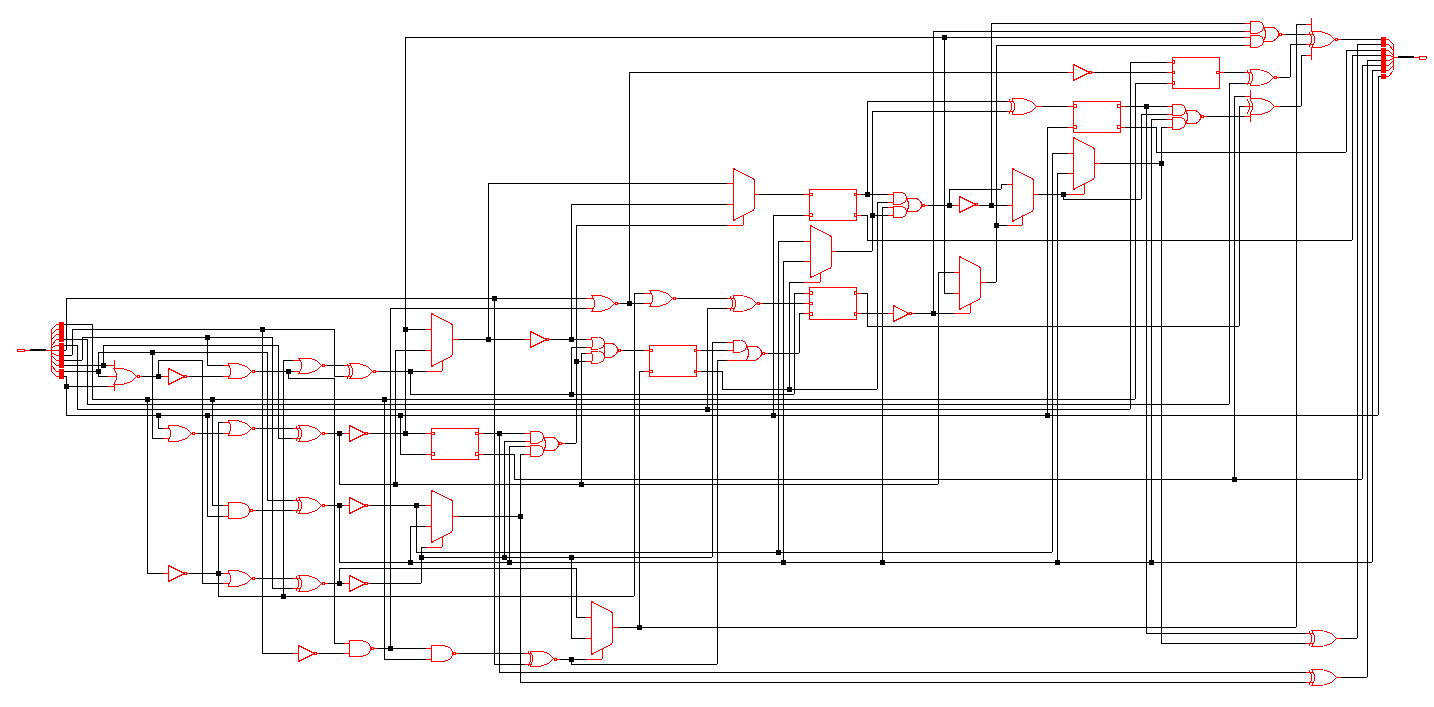
\includegraphics[width=1\textwidth]{img/Konstantenmultiplizierer_Encounter_sw.png}
  }
  \caption{12 Bit Konstantenmultiplizierer für $\frac{\sqrt{2}}{2} = 0,70711... \simeq 0,70703 = 010110101000_2$ in Encounter}
\end{figure}



\begin{table}[!ht]
 \caption{Vergleich Konstanten- mit regulärem Multiplizierer}
 \label{tab:VergleichMultiplizierer}
 \begin{tabular}{ccc}
 \hline
				& Konstantenmultiplizierer 	& regulärer Multiplizierer\\
  \hline	
  Gatter			& 27				& 175 \\
  Fläche (Prozess: 350nm)	& $\SI{6612}{\mu m^2}$		& $\SI{23261}{}$\\
  \hline
 \end{tabular}
\end{table}


Der Ausgang hat so wie der Eingang 13 Bit.

Auf Skript verweisen, mit dem ermittelt wurde, dass das die beste Annäherung an $\frac{\sqrt{2}}{2}$ ist.

Der vollständige Gate-Report befindet sich in Abschnitt \ref{src:rc_gate_report} auf Seite \pageref{src:rc_gate_report}



 
 \section{Entwickeln der 2D-DFT }

\section{Direkte Weiterverarbeitung der Zwischenergebnisse}
Um die Anzahl an Gattern und somit den Flächenbedarf zu reduzieren ist es das Ziel, die Ergebnisse der \gls{1d-dft} aus der 1. Berechnungsstufe im nächsten Schritt direkt als 
Eingangswerte für die \gls{2d-dft} zu verwenden. Auf diese Weise würden 64$\cdot$2$\cdot$12 Bit = 1536 Bit = 1,5kBit = 192 Byte an Speicher eingespart werden.

\subsection{Matrizenmultiplikation}

Um die nachfolgenden Abschnitte besser erörten zu können, soll zunächst die Matrizenmultiplikation besprochen werden.
Wie in Abbildung \ref{eq:grafikMatrizenmultiplikation} verdeutlicht, wird Element$(i,j)$ der Ergebnismatrix dadurch berechnet, dass die Elemente$(i,k)$ einer Zeile der 1. Matrix
mit den Elementn$(k,j)$ aus der zweiten Matrix multipliziert und die Werte aufsummiert werden. $i$ und $j$ sind für die Berechnung eines Elements konstant, während $k$ über alle
Elemente einer Zeile bzw. Spalte läuft.

\begin{center}
 
\begin{minipage}{0.2\textwidth}
 \begingroup
 \renewcommand*{\arraystretch}{1.1} % Zeilenabstand
 \renewcommand*{\arraycolsep}{0.0pt} % Spaltenabstand

 \[
    \begin{bmatrix}
    \tikzmark{varrowtopleft} \myBlackBox  	& \myBlackBox 		& \myBlackBox 		& \tikzmark{varrowtopright} \myBlackBox \\
                             \myLightgrayBox 	& \myLightgrayBox 	& \myLightgrayBox 	& \myLightgrayBox \\
                             \myLightgrayBox 	& \myLightgrayBox	& \myLightgrayBox	& \myLightgrayBox \\
    \tikzmark{varrowbottom}  \myLightgrayBox 	& \myLightgrayBox 	& \myLightgrayBox 	& \myLightgrayBox 
   \end{bmatrix}
 \]
 \endgroup
  \tikz[overlay,remember picture] {
  \draw[->] ([yshift=1.5ex,xshift=-2ex]varrowtopleft) -- ([xshift=-2ex]varrowbottom)
            node[midway,left] {$i$};
  \draw[->] ([xshift=2ex,yshift=4ex]varrowtopleft) -- ([yshift=4ex]varrowtopright)
            node[midway,above] {$k$};
}
\end{minipage}
\begin{minipage}{0.1\textwidth}
 \hspace{-.5cm}
 \[
  \cdot
 \]
\end{minipage}
\begin{minipage}{0.2\textwidth}
 \begingroup
 \renewcommand*{\arraystretch}{0.0} % Zeilenabstand
 \renewcommand*{\arraycolsep}{0.8pt} % Spaltenabstand
 \[
   \begin{bmatrix}
    \tikzmark{varrowtopleft} \myLightgrayBoxHigh & \myBlackBoxHigh & \myLightgrayBoxHigh & \tikzmark{varrowtopright} \myLightgrayBoxHigh \\
                             \myLightgrayBoxHigh & \myBlackBoxHigh & \myLightgrayBoxHigh & \myLightgrayBoxHigh \\
                             \myLightgrayBoxHigh & \myBlackBoxHigh & \myLightgrayBoxHigh & \myLightgrayBoxHigh \\
    \tikzmark{varrowbottom}  \myLightgrayBoxHigh & \myBlackBoxHigh & \myLightgrayBoxHigh & \myLightgrayBoxHigh 
   \end{bmatrix}
 \]
 \endgroup
   \tikz[overlay,remember picture] {
  \draw[->] ([yshift=1.5ex,xshift=-2ex]varrowtopleft) -- ([xshift=-2ex]varrowbottom)
            node[midway,left] {$k$};
  \draw[->] ([xshift=2ex,yshift=4ex]varrowtopleft) -- ([yshift=4ex]varrowtopright)
            node[midway,above] {$j$};
}
\end{minipage}
\begin{minipage}{0.05\textwidth}
 \[
  =
 \]
\end{minipage}
\begin{minipage}{0.3\textwidth}
\begingroup
\renewcommand*{\arraystretch}{1.1} % Zeilenabstand
\renewcommand*{\arraycolsep}{0.8pt} % Spaltenabstand
\begin{align}\label{eq:grafikMatrizenmultiplikation}
   \begin{bmatrix}
    \tikzmark{varrowtopleft} \myLightgrayBox 	& \myBlackBox		& \myLightgrayBox 	& \tikzmark{varrowtopright} \myLightgrayBox \\
                             \myLightgrayBox 	& \myLightgrayBox 	& \myLightgrayBox 	& \myLightgrayBox \\
                             \myLightgrayBox 	& \myLightgrayBox 	& \myLightgrayBox 	& \myLightgrayBox \\
    \tikzmark{varrowbottom}  \myLightgrayBox 	& \myLightgrayBox 	& \myLightgrayBox 	& \myLightgrayBox 
   \end{bmatrix}
 \end{align} 
 \endgroup
    \tikz[overlay,remember picture] {
  \draw[->] ([yshift=1.5ex,xshift=-2ex]varrowtopleft) -- ([xshift=-2ex]varrowbottom)
            node[midway,left] {$i$};
  \draw[->] ([xshift=2ex,yshift=4ex]varrowtopleft) -- ([yshift=4ex]varrowtopright)
            node[midway,above] {$j$};
}
\end{minipage}
\end{center}


\subsection{Veranschaulichung 2D-DFT als Matrizenmultiplikation}

Mathematisch wird die 2D-DFT als

\begin{align}
 X &= W \cdot x \cdot W \\
     &= X^* \cdot W
\end{align}

beschrieben. Es wird also erst die 1D-DFT berechnet und die sich daraus ergebende Matrix $X^*$ (Abb. \ref{eq:matrix_F1}) wird anschließend mit der Twiddlefaktor-Matrix $W$ 
multipliziert. Man könnte es auch als zweite 1D-DFT betrachten, bei der Twiddlefaktor-Matrix und Eingangsmatrix vertauscht sind.

Veranschaulicht wird dies in den Abbildungen \ref{eq:matrix_F1} und \ref{eq:matrix_F2}.


\begin{center}
 
\begin{minipage}{0.2\textwidth}
 \begingroup
 \renewcommand*{\arraystretch}{1.1} % Zeilenabstand
 \renewcommand*{\arraycolsep}{0.0pt} % Spaltenabstand

 \[
  \stackrel{\mbox{$W$}}{
   \begin{bmatrix}
    \myBlackBox 	& \myBlackBox 		& \myBlackBox 		& \myBlackBox \\
    \myLightgrayBox 	& \myLightgrayBox 	& \myLightgrayBox 	& \myLightgrayBox \\
    \myLightgrayBox 	& \myLightgrayBox	& \myLightgrayBox	& \myLightgrayBox \\
    \myLightgrayBox 	& \myLightgrayBox 	& \myLightgrayBox 	& \myLightgrayBox 
   \end{bmatrix}
  }
 \]
 \endgroup
\end{minipage}
\begin{minipage}{0.05\textwidth}
 \[
  \cdot
 \]
\end{minipage}
\begin{minipage}{0.2\textwidth}
 \begingroup
 \renewcommand*{\arraystretch}{0.0} % Zeilenabstand
 \renewcommand*{\arraycolsep}{0.8pt} % Spaltenabstand

 \[
  \stackrel{\mbox{$x$}}{
   \begin{bmatrix}
    \myBlackBoxHigh 	& \myBlackBoxHigh 	& \myBlackBoxHigh 	& \myBlackBoxHigh \\
    \myBlackBoxHigh 	& \myBlackBoxHigh 	& \myBlackBoxHigh 	& \myBlackBoxHigh \\
    \myBlackBoxHigh 	& \myBlackBoxHigh 	& \myBlackBoxHigh 	& \myBlackBoxHigh \\
    \myBlackBoxHigh 	& \myBlackBoxHigh 	& \myBlackBoxHigh 	& \myBlackBoxHigh 
   \end{bmatrix}
  }
 \]
 \endgroup
\end{minipage}
\begin{minipage}{0.05\textwidth}
 \[
  =
 \]
\end{minipage}
\begin{minipage}{0.3\textwidth}
\begingroup
\renewcommand*{\arraystretch}{1.1} % Zeilenabstand
\renewcommand*{\arraycolsep}{0.8pt} % Spaltenabstand
\begin{align}\label{eq:matrix_F1}
  \stackrel{\mbox{$X^*$}}{
   \begin{bmatrix}
    \myBlackBox 	& \myBlackBox 		& \myBlackBox 		& \myBlackBox \\
    \myLightgrayBox 	& \myLightgrayBox 	& \myLightgrayBox 	& \myLightgrayBox \\
    \myLightgrayBox 	& \myLightgrayBox 	& \myLightgrayBox 	& \myLightgrayBox \\
    \myLightgrayBox 	& \myLightgrayBox 	& \myLightgrayBox 	& \myLightgrayBox 
   \end{bmatrix}
  }
\end{align}

 
 \endgroup
\end{minipage}
\end{center}


\begin{center}
 
\begin{minipage}{0.2\textwidth}
 \begingroup
 \renewcommand*{\arraystretch}{1.1} % Zeilenabstand
 \renewcommand*{\arraycolsep}{0.0pt} % Spaltenabstand

 \[
  \stackrel{\mbox{$X^*$}}{
   \begin{bmatrix}
    \myBlackBox 	& \myBlackBox 		& \myBlackBox 		& \myBlackBox \\
    \myLightgrayBox 	& \myLightgrayBox 	& \myLightgrayBox 	& \myLightgrayBox \\
    \myLightgrayBox 	& \myLightgrayBox	& \myLightgrayBox	& \myLightgrayBox \\
    \myLightgrayBox 	& \myLightgrayBox 	& \myLightgrayBox 	& \myLightgrayBox 
   \end{bmatrix}
  }
 \]
 \endgroup
\end{minipage}
\begin{minipage}{0.05\textwidth}
 \[
  \cdot
 \]
\end{minipage}
\begin{minipage}{0.2\textwidth}
 \begingroup
 \renewcommand*{\arraystretch}{0.0} % Zeilenabstand
 \renewcommand*{\arraycolsep}{0.8pt} % Spaltenabstand

 \[
  \stackrel{\mbox{$W$}}{
   \begin{bmatrix}
    \myBlackBoxHigh 	& \myBlackBoxHigh 	& \myBlackBoxHigh 	& \myBlackBoxHigh \\
    \myBlackBoxHigh 	& \myBlackBoxHigh 	& \myBlackBoxHigh 	& \myBlackBoxHigh \\
    \myBlackBoxHigh 	& \myBlackBoxHigh 	& \myBlackBoxHigh 	& \myBlackBoxHigh \\
    \myBlackBoxHigh 	& \myBlackBoxHigh 	& \myBlackBoxHigh 	& \myBlackBoxHigh 
   \end{bmatrix}
  }
 \]
 \endgroup
\end{minipage}
\begin{minipage}{0.05\textwidth}
 \[
  =
 \]
\end{minipage}
\begin{minipage}{0.3\textwidth}
\begingroup
\renewcommand*{\arraystretch}{1.1} % Zeilenabstand
\renewcommand*{\arraycolsep}{0.8pt} % Spaltenabstand
\begin{align}\label{eq:matrix_F2}
  \stackrel{\mbox{$X$}}{
   \begin{bmatrix}
    \myBlackBox 	& \myBlackBox 		& \myBlackBox 		& \myBlackBox \\
    \myLightgrayBox 	& \myLightgrayBox 	& \myLightgrayBox 	& \myLightgrayBox \\
    \myLightgrayBox 	& \myLightgrayBox 	& \myLightgrayBox 	& \myLightgrayBox \\
    \myLightgrayBox 	& \myLightgrayBox 	& \myLightgrayBox 	& \myLightgrayBox 
   \end{bmatrix}
  }
 \end{align}
 \endgroup
\end{minipage}
\end{center}


\section{Optimieren der 8x8-DFT}

Aus der anfänglichen Implementation bei der alle Werte einer Berechnung die entweder mit $+\frac{\sqrt{2}}{2}$ oder $-\frac{\sqrt{2}}{2}$ multipliziert werden müssen 
einzelnd berechnet werden, wird sinngemäß der gemeinsame Faktor ausgeklammert, sodass nur noch jeweils eine Multiplikation erforderlich ist.





\section{Ungleiche Bitbreiten bei gerader / ungerader Zeile}

Berechnung ungerader Zeilen am Beispiel der ersten:
\begin{center}
$a_{k0} + a_{k1} + a_{k2} + a_{k3} + a_{k4} + a_{k5} + a_{k6} + a_{k7}$\\
\end{center}
%\hrule
\vspace{0.5cm}

\begin{tabular}{ccccccccc}
Takt&\multicolumn{6}{l}{ } & & Bit\\
&$\underbrace{a_{k0} + a_{k1}}$ &  &$ \underbrace{a_{k2} + a_{k3}}$ &  &$\underbrace{a_{k4} + a_{k5}}$ &  &$\underbrace{a_{k6} + a_{k7}}$ & 12\\
2&\multicolumn{7}{l}{$\hspace{0.65cm} \Downarrow \hspace{2.3cm} \Downarrow \hspace{2.3cm} \Downarrow \hspace{2.3cm}\Downarrow$}&\\
&\multicolumn{3}{c}{$\underbrace{sum\_s1\_1 \quad + \quad sum\_s1\_2}$} & & \multicolumn{3}{c}{$\underbrace{sum\_s1\_3 \quad + \quad sum\_s1\_4}$} & 13\\
3&\multicolumn{3}{c}{$\Downarrow$} & & \multicolumn{3}{c}{$\Downarrow$}&\\
&\multicolumn{7}{c}{$\underbrace{sum\_s2\_1 \quad  \quad \quad \quad + \quad \quad \quad  \quad sum\_s2\_2}$} & 14\\
4&\multicolumn{7}{c}{$\Downarrow$}&\\
&\multicolumn{7}{c}{$sum\_s3\_1$} & 15\\
&\end{tabular}

\vspace{0.5cm}

$\Rightarrow$ 3 Takte, 1. und 5. Leerlauf

\vspace{1cm}

Berechnung gerader Zeilen am Beispiel der zweiten:
 \begin{center} 
 $a_0 - x_1 + x_0 - b_2 + x_2 - x_3 + a_4 - x_5 + x_4 - b_6 + x_6 - x_7$\\
 \end{center}
 %\hrule
 
 \vspace{0.3cm}

\begin{tabular}{ccccccccccccc}
Takt&\multicolumn{11}{c}{}&Bit\\
&$\underbrace{a_0 - x_1}$ &  &$ \underbrace{x_0 - b_2}$ &  &$\underbrace{x_2 - x_3}$ &  &$\underbrace{a_4 - x_5}$ &  &$\underbrace{x_4 - b_6}$ &  &$\underbrace{x_6 - x_7}$&12\\
2&\multicolumn{11}{l}{$\hspace{0.5cm} \Downarrow \hspace{1.75cm} \Downarrow \hspace{1.8cm} \Downarrow \hspace{1.75cm}\Downarrow \hspace{1.75cm}\Downarrow \hspace{1.8cm}\Downarrow$}&\\
&\multicolumn{3}{c}{$\underbrace{s1\_1 \quad + \quad s1\_2}$} & & \multicolumn{3}{c}{$\underbrace{s1\_3 \quad + \quad s1\_4}$} & & \multicolumn{3}{c}{$\underbrace{s1\_5 \quad + \quad s1\_6}$}&13\\
3&\multicolumn{3}{c}{$\Downarrow$} & & \multicolumn{3}{c}{$\Downarrow$} & & \multicolumn{3}{c}{$\Downarrow$}&\\
&\multicolumn{7}{c}{$\underbrace{s2\_1 \quad  \quad \quad \quad + \quad \quad \quad  \quad s2\_2}$} & & \multicolumn{3}{c}{$s2\_3$}&14\\
4&\multicolumn{7}{c}{$\Downarrow$}& & \multicolumn{3}{c}{$\Downarrow$}&\\
&\multicolumn{7}{c}{$s3\_1$}& & \multicolumn{3}{c}{$\Downarrow$}&15\\
&\multicolumn{2}{c}{}& \multicolumn{9}{c}{$\underbrace{\quad \quad \quad \quad \quad \quad \quad \quad \quad \quad \quad \quad \quad \quad \quad \quad \quad}$}&\\
5&\multicolumn{2}{c}{}& \multicolumn{9}{c}{$\Downarrow$}&\\
&\multicolumn{2}{c}{}& \multicolumn{9}{c}{$s4\_1$}&16
\end{tabular}


$\Rightarrow$ 5 Takte, 1. Multiplikationen, 2.-5. Additionen

 

\section{Struktogramm}

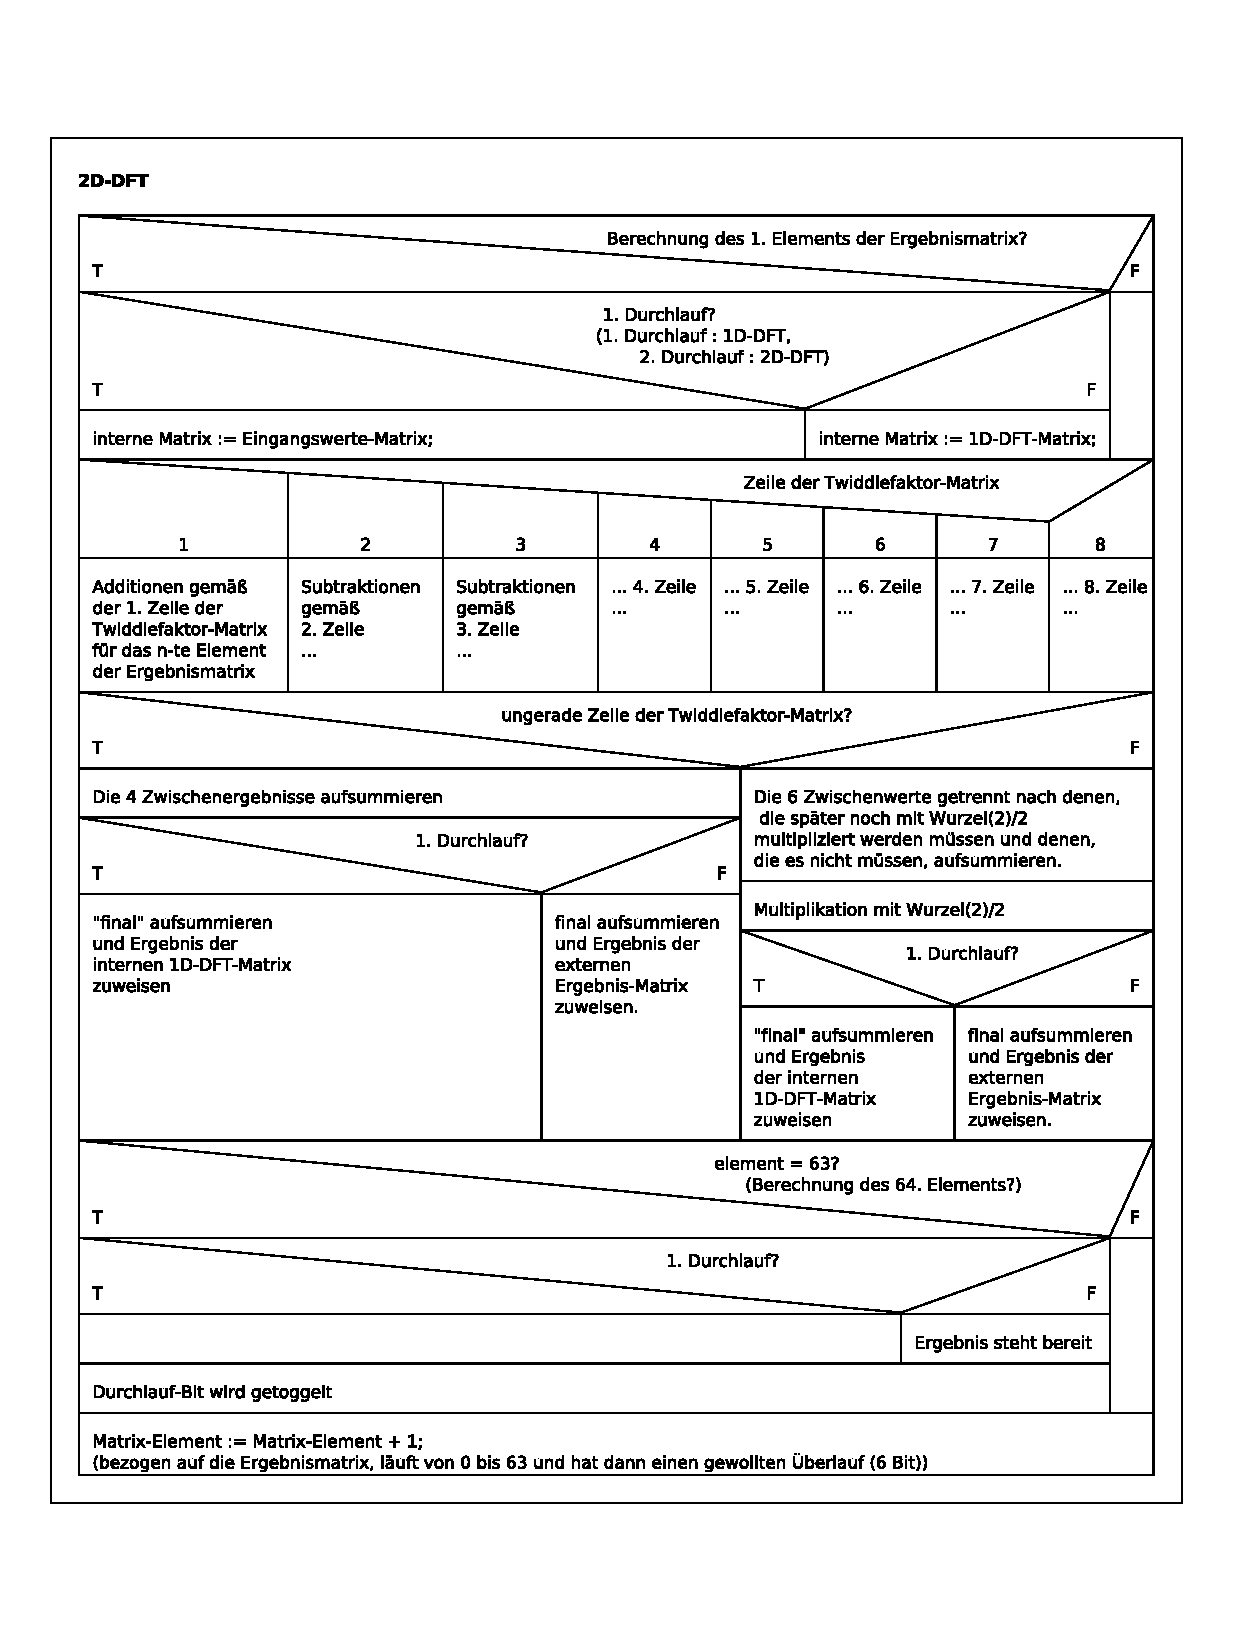
\includepdf{content/Struktogramm.pdf}

\section{Automatengraf}

\begin{center}
 
\begin{tikzpicture}[->,>=stealth',shorten >=1pt,auto,node distance=4.5cm,
                    semithick,initial text=nReset, initial where=above]
  \tikzstyle{every state}=[fill=white, text=black]
  %\tikzstyle{every initial where}=[above]
  

  \node[initial,state, circle split,minimum size=70pt] (A)                   {Idle};
  \node[state, circle split, minimum size=70pt]         (B) [below right of=A]{Twiddle\_Calc};
  \node[state, circle split, minimum size=70pt]         (C) [below right of=B]      {Additions\_1};
  \node[state, circle split, minimum size=70pt]         (D) [below of=C] {Additions\_2};
  \node[state, circle split, minimum size=70pt]         (E) [below left of=D] {Const\_mult};
  \node[state, circle split, minimum size=70pt]         (F) [above left of=E]      {Additions\_3};
  \node[state, circle split, minimum size=70pt]         (G) [above of=F]      {set\_ready\_bit};

  
   \path (A) edge (B) 
         (A) [loop left] edge(A)
         (B) [bend left=10] edge (C)
         (C) edge (D)
         (D) edge (B)
         (D) edge (E)
         (E) edge (F)
         (F) [bend right=10] edge (B)
         (F) [bend left=10] edge (G)
         (G) edge (B);
\end{tikzpicture}
\end{center}




%\begin{landscape}
 


% Define block styles
\tikzstyle{decision} = [diamond,                    draw, fill=blue!20, text width=6em, text badly centered, node distance=4cm, inner sep=0pt]
\tikzstyle{block} =    [rectangle, rounded corners, draw, fill=blue!20, text width=5em, text centered,       node distance=4cm, minimum height=5em, minimum width=7em]
\tikzstyle{smallblock} =    [rectangle, rounded corners, draw, fill=blue!20, text width=5em, text centered,       node distance=4cm, minimum height=2em, minimum width=3.5em]
\tikzstyle{wideblock} =    [rectangle, rounded corners, draw, fill=blue!20, text width=7em, text centered,       node distance=4cm, minimum height=5em, minimum width=7em]
\tikzstyle{verywideblock} =    [rectangle, rounded corners, draw, fill=blue!20, text width=15em, text centered,       node distance=4cm, minimum height=4em, minimum width=15em]
\tikzstyle{textblock} =    [rectangle, rounded corners, draw, fill=blue!20, text width=12em, text centered,       node distance=4cm, minimum height=4em, minimum width=10em]
\tikzstyle{dot}=[draw,shape=circle]

\tikzstyle{arrowline} = [draw, -latex']


    
\begin{tikzpicture}[auto, node distance = 1cm and 1cm, initial text=POR, initial where=above]
    % Place nodes
    \node [initial, smallblock] (start) {Idle};
    \node [decision, below of=start, node distance=3cm] (init) {IDFT?};
    \node [block, below right of=init, node distance=3cm] (Zeilenindex) {Zeilenindex tauschen};
    \coordinate[below of=init, node distance=3.5cm](Punkt_0);
    \node [decision, below of=Punkt_0, node distance=2cm] (Element_1) {Berechnung 1. Element?};
    \coordinate [right of=Element_1, node distance=4cm](c1);
    \node [decision, below of=c1, node distance=2cm] (Berechnung_1D_1) {Berechnung 1D-DFT?};
    
    \node [block, below of=Berechnung_1D_1, node distance=3cm] (überschreiben_mit_eingangswerten) {Zwischen- werte := 1D-DFT-Werten};
    \node [block, right of=überschreiben_mit_eingangswerten, node distance=4cm] (überschreiben_mit_1D_Werten) {Zwischen- werte := Eingangswerte};
    \node [block, left of=überschreiben_mit_eingangswerten, node distance=4cm] (Werte_beibehalten) {Zwischen- werte := Zwischen- werte};
    
    \node [dot, fill, inner sep=1pt, below of=überschreiben_mit_eingangswerten,node distance=1.5cm] (Punkt_1){};
    \node [decision,                 below of=Punkt_1,node distance=2cm] (Zustandsabfrage) {Zeilen- abfrage};
    
    \node [dot, fill, inner sep=1pt, below of=Zustandsabfrage,node distance=2cm] (Punkt_2){};
    \coordinate[below of=Punkt_2, node distance=0.5cm](Punkt_3);
    
    \node [textblock, right of=Punkt_2, node distance=3cm] (Zeile_1){Berechnungen entsprechend Zeile 1 der Twiddlefaktor-Matrix};
      
    \coordinate[below of=Punkt_3](Punkt_4);
    \coordinate[below of=Punkt_4,node distance=0.5cm] (Punkt_5);
    \node [textblock, right of=Punkt_5, node distance=3cm] (Zeile_8){Berechnungen entsprechend Zeile 8 der Twiddlefaktor-Matrix};
    
    \coordinate[right of=Zeile_1, node distance=3cm](Punkt_6);
    \coordinate[below of=Punkt_6, node distance=0.5cm] (Punkt_7);
    \node [dot, fill, inner sep=0.01pt, right of=Zeile_8, node distance=3cm](Punkt_9){};
    \coordinate[above of=Punkt_9, node distance=0.5cm] (Punkt_8);
    \coordinate[below of=Punkt_9, node distance=2cm](Punkt_10);
    \coordinate[left of=Punkt_10, node distance=12cm](Punkt_return_1);
    
    \coordinate[right of=init, node distance=8cm](textfeld);
    \node [draw, text, fill=white, above of=textfeld, node distance=1.3cm](tf){Zustand 2: Twiddle\_Calc};
    \coordinate[right of=start, node distance=7.1cm](textfeld2);
    \node [draw, text, fill=white, above of=textfeld2, node distance=1cm](tf2){Zustand 1: Idle};
    \node [dot, fill, inner sep=1pt, above of=init, node distance=1.7cm](Knoten_init){};
    
   % Koordinaten für Hintergrund
   \coordinate [above of=start, node distance=1.5cm](b11);
   \coordinate [right of=start, node distance=13.6cm](b12);
   \coordinate [below of=start, node distance=1cm](b13);
   \coordinate [left of=start, node distance=1.5cm](b14);
    
    % Draw edges
    \draw (start) -- (Knoten_init);
    \path [arrowline] (Knoten_init) -- (init);
    \path [arrowline] (init) -| node [near start] {ja} (Zeilenindex);
    \draw (Zeilenindex) |- (Punkt_0);    
    \draw (init) -- node [left, near start] {nein} (Punkt_0);
    \path [arrowline] (Punkt_0) -- (Element_1);
    \path [arrowline] (Element_1) -| node [near start] {ja} (Berechnung_1D_1);
    \path [arrowline] (Berechnung_1D_1) -- node [near start] {nein} (überschreiben_mit_eingangswerten);
    \path [arrowline] (Berechnung_1D_1) -| node [near start] {ja} (überschreiben_mit_1D_Werten);
    \path [arrowline] (Element_1) -- node [left, near start] {nein} (Werte_beibehalten);
    
    \draw (Werte_beibehalten) |- (Punkt_1);
    \draw (überschreiben_mit_eingangswerten) -- (Punkt_1);
    \draw (überschreiben_mit_1D_Werten) |- (Punkt_1);
    \path [arrowline] (Punkt_1) -- (Zustandsabfrage);
    \draw (Zustandsabfrage) -- (Punkt_2);
    
    \path [arrowline] (Punkt_2) -- (Zeile_1);
    \draw (Punkt_2) -- (Punkt_3);
    \draw [loosely dotted] (Punkt_3) -- (Punkt_4);
    \draw (Punkt_4) -- (Punkt_5);
    \path [arrowline](Punkt_5) -- (Zeile_8);
    
    \draw (Zeile_1) -- (Punkt_6);
    \draw (Punkt_6) -- (Punkt_7);
    \draw [loosely dotted] (Punkt_7) -- (Punkt_8);
    \draw (Punkt_8) -- (Punkt_9);
    \draw (Zeile_8) -- (Punkt_9);
    \draw (Punkt_9) -- (Punkt_10);
    \draw (Punkt_return_1) |- (Knoten_init);
    \path (start) [loop right] edge (start);
    
     \begin{pgfonlayer}{background}
      \filldraw [fill=gray!20, draw=gray!15]
        (b11.north -| b12.west)  rectangle (b13.south -| b14.east);
     \end{pgfonlayer}

    
\end{tikzpicture}

\begin{tikzpicture}[auto, node distance = 1cm and 1cm, initial text="", initial where=above]



\node [initial, decision] (gerade_Zeile_1) {gerade Zeile?};
\node [wideblock, below left of=gerade_Zeile_1] (gerade_Zeile_1_aufsummieren) {Zwischenwerte paarweise aufsummieren};
\node [wideblock, below right of=gerade_Zeile_1] (ungerade_Zeile_1_aufsummieren) {Zwischenwerte paarweise aufsummieren, zu multiplizierende getrennt};
\node [dot, fill, inner sep=1pt, below of=gerade_Zeile_1, node distance=5cm](Punkt_1){};


\node [decision, below of=Punkt_1, node distance=4cm] (gerade_Zeile_2) {gerade Zeile?};
\coordinate [left of=gerade_Zeile_2, node distance=3.5cm] (Punkt_gerade_Zeile_2);
\coordinate [right of=gerade_Zeile_2, node distance=3.5cm] (Punkt_gerade_Zeile_2_2);

\node [block, below of=Punkt_gerade_Zeile_2, node distance=3cm] (ungerade_Zeile_2_aufsummieren) {Letztes Paar aufsummieren};
\node [block, below of=Punkt_gerade_Zeile_2_2, node distance=3cm] (gerade_Zeile_2_aufsummieren) {Letztes Multiplikationspaar aufsummieren};
\node [decision, below of=ungerade_Zeile_2_aufsummieren, node distance=3cm] (Berechnung_1D_2) {Berechnung 1D-DFT?};

\node [block, below left of=Berechnung_1D_2, node distance=3.2cm] (Werte_extern_speichern_1) {Werte in (externe) 2D-DFT-Matrix speichern};
\node [block, below right of=Berechnung_1D_2, node distance=3.2cm] (Werte_intern_speichern_1) {Werte in (interne) 1D-DFT-Matrix speichern};
\coordinate [below of=Werte_extern_speichern_1, node distance=2cm](Punkt_3);
\coordinate [below of=Werte_intern_speichern_1, node distance=2cm](Punkt_4);

\coordinate (Middle_2) at ($(Punkt_3)!0.5!(Punkt_4)$);
\node [dot, fill, inner sep=1pt,  above of=Middle_2, node distance=0cm] (Middle_2_dot){};
\node [block, below of=Middle_2, node distance=1.5cm] (Matrix_Element_plus_1_1) {Matrix-Element += 1};
\coordinate [below=of Matrix_Element_plus_1_1](Punkt_5);

\coordinate [left of=Punkt_5, node distance=6cm] (Punkt_unten_links);
\node [dot, fill, inner sep=1pt, above of=Punkt_unten_links, node distance=0.5cm](Knoten_unten_links){};
\coordinate [below of=gerade_Zeile_2_aufsummieren, node distance=10.8cm] (Punkt_unten_rechts);
\coordinate [above of=Punkt_unten_links, node distance=25cm] (Punkt_oben_links);

 % Koordinaten für Hintergrund
 \coordinate [above of=gerade_Zeile_1, node distance=2.1cm](b11);
 \coordinate [right of=ungerade_Zeile_1_aufsummieren, node distance=3.3cm](b12);
 \coordinate [above of=gerade_Zeile_2, node distance=3cm](b13);
 \coordinate [left of=gerade_Zeile_1_aufsummieren, node distance=6cm](b14);
 
 % Text
 \coordinate[left of=gerade_Zeile_1, node distance=5.5cm](textfeld);
 \node [draw, text, fill=white, above of=textfeld, node distance=1.2cm](tf){Zustand 3: Summation\_1};
 
 \node [draw, text, below of=textfeld, node distance=7cm](tf2){Zustand 4: Summation\_2}; 


\path [arrowline] (gerade_Zeile_1) -| node [above, near start] {nein} (gerade_Zeile_1_aufsummieren);
\path [arrowline] (gerade_Zeile_1) -| node [near start] {ja} (ungerade_Zeile_1_aufsummieren);
\draw (gerade_Zeile_1_aufsummieren) |- (Punkt_1);
\draw (ungerade_Zeile_1_aufsummieren) |- (Punkt_1); 
\path [arrowline] (Punkt_1) -- (gerade_Zeile_2);

\draw (gerade_Zeile_2) -- node [above, near start] {nein} (Punkt_gerade_Zeile_2);
\path [arrowline] (Punkt_gerade_Zeile_2) -| (ungerade_Zeile_2_aufsummieren);
\draw (gerade_Zeile_2) -- node [near start] {ja} (Punkt_gerade_Zeile_2_2);

\path [arrowline] (Punkt_gerade_Zeile_2_2) -| (gerade_Zeile_2_aufsummieren);
\path [arrowline] (ungerade_Zeile_2_aufsummieren) -- (Berechnung_1D_2);
\path [arrowline] (Berechnung_1D_2) -| node [above] {nein} (Werte_extern_speichern_1);
\path [arrowline] (Berechnung_1D_2) -| node [above] {ja} (Werte_intern_speichern_1);
\draw (Werte_extern_speichern_1) -- (Punkt_3);
\draw (Werte_intern_speichern_1) -- (Punkt_4);
\draw (Punkt_3) -- (Middle_2);
\draw (Punkt_4) -- (Middle_2);
\path [arrowline] (Middle_2) -- (Matrix_Element_plus_1_1);
\draw (Matrix_Element_plus_1_1) |- (Knoten_unten_links);
\draw (Punkt_unten_links) -- (Knoten_unten_links);
\path [arrowline] (Knoten_unten_links) -- (Punkt_oben_links);
\path [arrowline](gerade_Zeile_2_aufsummieren) -- (Punkt_unten_rechts);

 \begin{pgfonlayer}{background}
  \filldraw [fill=gray!20, draw=gray!5]
  (b11.north -| b12.west)  rectangle (b13.south -| b14.east);
 \end{pgfonlayer}


\end{tikzpicture}


\begin{tikzpicture}[auto, node distance = 1cm and 1cm, initial text="", initial where=above]
 \node [initial, verywideblock] (Multiplikation) {Multiplikation durchführen};
 \node [verywideblock, below of=Multiplikation, node distance=2.5cm] (letzte_Summation){Additionskomponente und Multiplikationskompnente aufsummieren};
 \node [decision, below of=letzte_Summation, node distance=3cm] (Berechnung_1D_3) {Berechnung 1D-DFT?};
 \node [block, below left of=Berechnung_1D_3, node distance=3.5cm] (Werte_extern_speichern_2) {Werte in (externe) 2D-DFT-Matrix speichern};
 \node [block, below right of=Berechnung_1D_3, node distance=3.5cm] (Werte_intern_speichern_2) {Werte in (interne) 1D-DFT-Matrix speichern};
 
 \node [dot, fill, inner sep=1pt, below of=Berechnung_1D_3, node distance=4cm](Knoten_berechnung_dft2){};
 \node [decision, below of=Knoten_berechnung_dft2, node distance=2cm] (Element_63) {Berechnung 63. Element};
 
 \coordinate [left of=Element_63, node distance=3cm] (links_neben_element_63);
 \node [dot, fill, inner sep=1pt, below of=links_neben_element_63, node distance=5.5cm] (Knoten_über_matrix_element_plus1_2) {};
 \node [block, below of=Knoten_über_matrix_element_plus1_2, node distance=1.6cm] (Matrix_Element_plus_1_2){Matrix-Element += 1};
 
 \node [decision, below right of=Element_63, node distance=3cm] (Berechnung_1D_4) {Berechnung 1D-DFT?};
 \node [block, below left of=Berechnung_1D_4, node distance=3cm] (dft_1d_2d_2) {DFT\_1D\_2D := 2D};
 \node [block, below right of=Berechnung_1D_4, node distance=3cm] (dft_1d_2d_1) {DFT\_1D\_2D := 1D};
 \node [block, below of=dft_1d_2d_1, node distance=3cm] (Matrix_Element_plus_1_3){Matrix-Element += 1};
 \node [block, below of=Matrix_Element_plus_1_3, node distance=3cm] (set_ready_bit) {Ready-Bit setzen};
 \coordinate [below of=set_ready_bit, node distance=1.5cm](unter_set_ready_bit);
 \coordinate [left of=unter_set_ready_bit, node distance=14cm](Punkt_unten_links);
 \node [dot, fill, inner sep=1pt, above of=Punkt_unten_links, node distance=3cm](knoten_für_plus_1){};
 \coordinate [above of=knoten_für_plus_1, node distance=21.5cm] (Punkt_oben_links);
 
 % Koordinaten für Hintergrund
 \coordinate [above of=Multiplikation, node distance=1.3cm](b11);
 \coordinate [right of=Multiplikation, node distance=5.8cm](b12);
 \coordinate [below of=Multiplikation, node distance=1.3cm](b13);
 \coordinate [left of=Multiplikation, node distance=9cm](b14);
 
 \coordinate [above of=set_ready_bit, node distance=1.3cm](b21);
 \coordinate [right of=set_ready_bit, node distance=1.6cm](b22);
 \coordinate [below of=set_ready_bit, node distance=1.3cm](b23);
 \coordinate [left of=set_ready_bit, node distance=13.2cm](b24);
 
  % Text
 \coordinate[left of=Multiplikation, node distance=6cm](textfeld);
 \node [draw, text, fill=white, above of=textfeld, node distance=0.5cm](tf){Zustand 5: Const\_Mult};
 \node [draw, text, fill=white, below of=textfeld, node distance=2cm](tf){Zustand 6: Summation\_3};
 \node [draw, text, fill=white, below of=textfeld, node distance=21.2cm](tf){Zustand 7: Set\_Ready\_Bit};
 
 
 \path [arrowline] (Multiplikation) -- (letzte_Summation);
 \path [arrowline] (letzte_Summation) -- (Berechnung_1D_3);
 \path [arrowline] (Berechnung_1D_3) -| node [above] {nein} (Werte_extern_speichern_2);
 \path [arrowline] (Berechnung_1D_3) -| node [above] {ja} (Werte_intern_speichern_2);
 \draw (Werte_extern_speichern_2) |- (Knoten_berechnung_dft2);
 \draw (Werte_intern_speichern_2) |- (Knoten_berechnung_dft2);
 \path [arrowline] (Knoten_berechnung_dft2) -- (Element_63);
 \draw (Element_63) -- node [above] {nein} (links_neben_element_63);
 \draw (links_neben_element_63) -- (Knoten_über_matrix_element_plus1_2);
 \draw (dft_1d_2d_2) |- (Knoten_über_matrix_element_plus1_2);
 \path [arrowline] (Knoten_über_matrix_element_plus1_2) -- (Matrix_Element_plus_1_2);
 \path [arrowline] (Berechnung_1D_4) -| node [above] {ja} (dft_1d_2d_2);
 
 \path [arrowline] (Element_63) -| node [above] {ja} (Berechnung_1D_4);
 \path [arrowline] (Berechnung_1D_4) -| node [above] {nein} (dft_1d_2d_1);
 \path [arrowline] (dft_1d_2d_1) -- (Matrix_Element_plus_1_3);
 \path [arrowline] (Matrix_Element_plus_1_3) -- (set_ready_bit);
 
 \draw (set_ready_bit) -- (unter_set_ready_bit);
 \draw (unter_set_ready_bit) -- (Punkt_unten_links);
 \path [arrowline] (Punkt_unten_links) -- (Punkt_oben_links);
 \draw (Matrix_Element_plus_1_2) |- (knoten_für_plus_1);
 
 \begin{pgfonlayer}{background}
  \filldraw [fill=gray!20, draw=gray!15]
  (b11.north -| b12.west)  rectangle (b13.south -| b14.east)
  (b21.north -| b22.west)  rectangle (b23.south -| b24.east);
 \end{pgfonlayer}

 
\end{tikzpicture}

%\end{landscape}

 
 
 

 
  
 \chapter{Evaluation}
 \section{Simulation}
 \subsection{NC Sim - positive Zahlendarstellung}
 
 \subsection{Anzahl benötigter Takte}
 Anhand der Simulation kann die Anzahl der vorausgesagten benötigten Takte verifiziert werden. 
 
 Nachdem \texttt{nReset} auf '1' gesetzt wird, werden die Eingangswerte
 eingelesen. Wenn dieser Vorgang abgeschlossen ist, geht \texttt{loaded} auf '1'. Mit der nächsten steigenden Taktflanke, in Bild \ref{pic:Simulationsdauer} bei 
 \SI{340}{ns}, beginnt die Berechnung
 der \gls{2d-dft}. Beendet ist sie, nachdem die Matrizenmultiplikation auf die Eingangswerte und anschließend auf die \gls{1d-dft}-Werte angewandt wurde. Also nach $2 \cdot 64$
 einzelnen Berechnungen. Wenn dies erfolgt ist, wird \texttt{result\_ready} auf '1' gesetzt. Dies geschieht bei \SI{20\,820}{ns}. Bei einer Taktfrequenz von $(\SI{40}{ns})^{-1}$
 (siehe \ref{src:dft8_optimiert_top}) ergeben sich so 512 Takte. Dies bestätigt auch der Edge Count, ebenfalls auf dem Bild zu sehen, welcher die Flanken des \texttt{clk}-Signals 
 zählt. In der Simulation ist zu erkennen, dass die Berechnung der Elemente 
 unterschiedlich viele Takte beansprucht. Hieran lässt sich ebenfalls sehen, dass die 1. (ungerade) Zeile weniger Takte gegenüber der 2. (geraden) Zeile benötigt. 
 
 %Auch in der Abbildung \ref{pic:Simulationsdauer} zu sehen ist, dass \texttt{element\_out} für 0 bis 7 weniger Takte einnimmt, als in den darauf folgenden 8. Dieses Muster
 %wiederholt sich und hat, wie in Abschnitt \ref{sec:berechnung_anzahl_takte} erläutert, damit zu tun, dass für die geraden
 
 \begin{figure}[htbp]
  \centering
  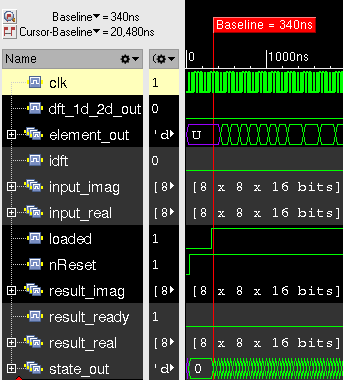
\includegraphics[width=0.58\textwidth]{img/Simulationsdauer_Anfang.png}
  \hfill
  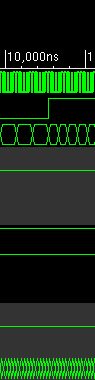
\includegraphics[width=0.161\textwidth]{img/Simulationsdauer_Mitte.png}
  \hfill
  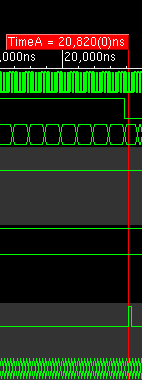
\includegraphics[width=0.241\textwidth]{img/Simulationsdauer_Ende.png}
  \caption{Simulations der 2D-DFT mit \texttt{NC Launch}}
  \label{pic:Simulationsdauer}
 \end{figure}

 \begin{figure}[htbp]
  \centering
  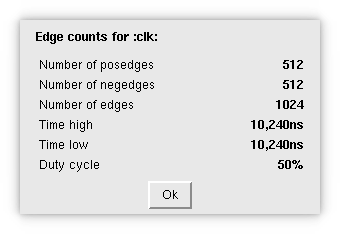
\includegraphics[width=0.6\textwidth]{img/Simulation_edge_count_clk.png}
  \caption{Edge Count für eine 2D-DFT}
 \end{figure}

 \subsection{Zeitabschätzung im Einsatz als ABS-Sensor}
 Anhand der nun bekannten Größe von 512 Takten kann ermittelt werden, ob diese Implemenatation vom zeitlichen Aspekt her akzeptabel ist.
 Da ein Einsatzszenario der ABS-Sensor ist, wird an dieser Stelle ein Blick hierauf geworfen. Da der ABS-Sensor an der Radnabe sitzt, wird 
 hierfür die Raddrehzahl benötigt. Um diese zu ermitteln, wird von einer maximalen Geschwindikeit von $v_{max}$ = 250\,KM/h ausgegangen. 
 Weiter wird ein realtiv kleiner Reifenumfang von ca. 1\,m angenommen. Als maximale Taktfrequenz des Sensors ist 1\,MHz vorgegeben.
 
 Der Reifen hat eine Breite von 175 cm, eine Flankenhöhe von 75\,$\%$ der Breite und die Felge einen Durchmesser von 14 Zoll. Somit errechnet sich der Reifenumfang
 gemäß (\ref{eq:Reifenumfang})
 
 \begin{align}\label{eq:Reifenumfang}
 \begin{split}
  U &= (\SI{175}{cm} \cdot 75\% \cdot 2 + 14 \cdot \SI{2.54}{cm})\cdot \pi\\
    &\simeq \SI{0,94}{m}
 \end{split}
 \end{align}

 In Gleichung \ref{eq:Umdrehungen} wird die Anzahl der Radumdrehungen bei maximaler Geschwindigkeit berechnet
 
 \begin{equation}\label{eq:Umdrehungen}
  \begin{split}
   RPM &= \dfrac{\dfrac{\SI{250}{Km/h}}{\SI{0,94}{m}}}{\SI{60}{sec}}\\
       &= \SI{4386}{\frac{U}{min}}\\
       &= \SI{73}{\frac{U}{sec}}
  \end{split}
 \end{equation}

 Durch die Taktfrequenz und die benötigten Takte kann in (\ref{eq:dft_sekunde}) die maximale Anzahl der 2D-DFTs pro Sekunde errechnet werden.
 
 \begin{equation}\label{eq:dft_sekunde}
  \begin{split}
   N_{DFT, sec} &= \frac{\SI{100}{MHz}}{\SI{512}{Takte}}\\
                &= 195312
  \end{split}
 \end{equation}

 Somit ist es nun möglich die unter diesen Voraussetzungen maximale Zahl der 2D-DFTs während einer Umdrehung zu bestimmen (\ref{eq:max_dft_umdrehung})
 
 \begin{equation}\label{eq:max_dft_umdrehung}
  \begin{split}
   N_{DFT,U}  &= \frac{\SI{195312}{\frac{2D-DFT}{sec}}}{\SI{73}{\frac{U}{sec}}}\\
              &= \SI{2675}{\frac{2D-DFT}{U}}
  \end{split} 
 \end{equation}

 Nun kann in (\ref{eq:max_dft_winkel}) gezeigt werden, dass bei einer Winkelauflösung von $1^\circ$ knapp 7,5 2D-DFTs berechnet werden könnten. Die Dauer liegt somit 
 gut im zeitlichen Rahmen, der vorganden ist. Darüber hinaus kann an dieser Stelle bereits gesagt werden, dass noch reichlich Zeit für andere Berechnungen vorhanden ist.
 
 \begin{equation}\label{eq:max_dft_winkel}
  \begin{split}
   N_{DFT,1^\circ} &= \frac{\SI{2675}{\dfrac{2D-DFT}{U}}}{360^\circ}\\
                   &= \SI{7,43}{\dfrac{2D-DFT}{1^\circ}}
  \end{split}
 \end{equation}

 
 Um eine Aussage über die restliche zur Verfügung stehenden Zeit bzw. Takte machen zu können, wird in Gleichung (\ref{eq:takte_pro_winkel}) gezeigt, dass pro Winkel 
 etwa 3800 Takte für Berechnungen zu Verfügung stehen. Somit ist gezeigt, dass für andere Aufgaben ausreichen Zeit vorhanden ist und die Implemenatation 
 erfolgreich ist.
 
 \begin{equation}\label{eq:takte_pro_winkel}
  \begin{split}
   N_{Takte, U} &= \frac{\SI{100}{MHz}}{73\dfrac{U}{sec}}\\
                &= 1,37\cdot 10^6 \frac{Takte}{Umdrehung}\\
   N_{Takte, 1^\circ} &= \frac{1,37\cdot 10^6 \dfrac{Takte}{Umdrehung}}{360^\circ}\\
                      &\simeq 3800 \ \textrm{Takte}
  \end{split}
 \end{equation}

 Da 512 etwa 13,5$\%$ von 3800 sind, resultiert hieraus, dass noch etwa 86,5$\%$ bzw. knapp 3300 Takte nutzbar sind.

 
 


 \section{Testumgebung}
 \subsection{Struktogramm des Testablaufs}
 \subsection{Reale Eingangswerte}
 
 \section{Chipdesign}
 \subsection{Anzahl Standardzellen}
 \subsubsection{Benötigte Standardzellen für 1D / 2D}
 \subsubsection{Benötigte Standardzellen bei 3 Lagen / 4 Lagen}
 \subsection{Visualisierung der Netzliste}
 \subsection{Floorplan, Padring}
 
 \chapter{Schlussfolgerungen}
 \section{Zusammenfassung}
 \section{Bewertung und Fazit}
 Es konnte eine effiziente Berechnung implementiert werden, die der FFT in nichts nachsteht. Wenn nicht die Ausgangssituation gewesen wäre, dass eine möglichst flexibel gehaltene
 Matrixmultiplikation erstrebenswert ist, hätte auch eine FFT, dessen Berechnungsvorschrift bekannt ist, implementiert werden können. Für DFT anderer Größe als $2^N$ gilt dies nicht.
 
 
 \section{Ausblick}
 
 
 \printglossary[title={Abkürzungsverzeichnis}] 
 
 \listoffigures
 \addcontentsline{toc}{chapter}{\listfigurename}

 \listoftables
 \addcontentsline{toc}{chapter}{\listtablename}

 
 \printbibliography
 \addcontentsline{toc}{chapter}{Literatur}
 
 \chapter{Anhang}
  \section{Skript zur Bewertung von Twiddlefaktormatrizen}
 \lstinputlisting[language=matlab, caption={Octave-Skript zur Bewertung unterschiedlicher DCT-Twiddlefaktormatrizen}, label=src:dct_bewertung]{../octave/dct_bewertung.m}
 \lstinputlisting[language=matlab, caption={Octave-Skript zur Bewertung unterschiedlicher DFT-Twiddlefaktormatrizen}, label=src:dft_bewertung]{../octave/dft_bewertung.m}
 \section{Gate-Report des 12 Bit Konstatenmultiplizierers}
 \lstinputlisting[language=matlab, caption={RC Gate-Report}, label=src:rc_gate_report]{Skripte/Konstantenmultiplizierer_gate_report.txt}

 \section{Twiddlefaktormatrix im S1Q10-Format}
 \lstinputlisting[language=matlab, caption={Erstellen der Twiddlefaktormatrix-Datei}, label=src:twiddle2file]{Skripte/Matlab/twiddle2file.m}
 \lstinputlisting[language=matlab, caption={Erzeugen der Twiddlefaktormatrix}, label=src:twiddle_coefficients]{Skripte/Matlab/twiddle_coefficients.m}
 \lstinputlisting[language=matlab, caption={Dezimalzahl nach S1Q10 konvertieren}, label=src:dec_to_s1q10]{Skripte/Matlab/dec_to_s1q10.m}
 \lstinputlisting[language=matlab, caption={Bildung des 2er-Komplements}, label=src:zweier_komplement]{Skripte/Matlab/zweier_komplement.m}
 \lstinputlisting[language=matlab, caption={Binär-Vektor in Binär-Integer umwandeln}, label=src:bit_vector2integer]{Skripte/Matlab/bit_vector2integer.m}
 \lstinputlisting[language=matlab, caption={Kontroll-Skript für S1Q10 nach Dezimal}, label=src:s1q10_to_dec]{Skripte/Matlab/s1q10_to_dec.m}
 

 %\section{Ausmultiplizieren der 8x8 DFT}\label{anhang:ausmultiplizieren}


\vspace{1cm}

\begingroup
\renewcommand*{\arraystretch}{1.1} % Zeilenabstand
\renewcommand*{\arraycolsep}{5.5pt} % Spaltenabstand
$\left[
\begin{array}{rcrcrcrc}
  \textcolor{green}{1+j0}	& \textcolor{green}{1+j0}					& \textcolor{green}{1+j0}	& \textcolor{green}{1+j0}					& \textcolor{green}{1+j0}	& \textcolor{green}{1+j0} 					& \textcolor{green}{1+j0}	& \textcolor{green}{1+j0} \\
  \textcolor{blue}{1+j0}	& \textcolor{blue}{\frac{\sqrt{2}}{2}+j\frac{\sqrt{2}}{2}}	& \textcolor{blue}{0+j1}	& \textcolor{blue}{-\frac{\sqrt{2}}{2}+j\frac{\sqrt{2}}{2}}	& \textcolor{blue}{-1+j0}	& \textcolor{blue}{-\frac{\sqrt{2}}{2}-j\frac{\sqrt{2}}{2}} 	& \textcolor{blue}{0-j1}	& \textcolor{blue}{\frac{\sqrt{2}}{2}-j\frac{\sqrt{2}}{2}} \\
  \textcolor{red}{1+j0}		& \textcolor{red}{0+j1}						& \textcolor{red}{-1+j0}	& \textcolor{red}{0-j1}						& \textcolor{red}{1+j0}		& \textcolor{red}{0+j1} 					& \textcolor{red}{-1+j0}	& \textcolor{red}{0-j1} \\
  \textcolor{lila}{1+j0}	& \textcolor{lila}{-\frac{\sqrt{2}}{2}+j\frac{\sqrt{2}}{2}}	& \textcolor{lila}{0-j1}	& \textcolor{lila}{\frac{\sqrt{2}}{2}+j\frac{\sqrt{2}}{2}}	& \textcolor{lila}{-1+j0}	& \textcolor{lila}{\frac{\sqrt{2}}{2}-j\frac{\sqrt{2}}{2}} 	& \textcolor{lila}{0+j1}	& \textcolor{lila}{-\frac{\sqrt{2}}{2}-j\frac{\sqrt{2}}{2}} \\
  \textcolor{cinnamon}{1+j0}	& \textcolor{cinnamon}{-1+j0}					& \textcolor{cinnamon}{1+j0}	& \textcolor{cinnamon}{-1+j0}					& \textcolor{cinnamon}{1+j0}	& \textcolor{cinnamon}{-1+j0} 					& \textcolor{cinnamon}{1+j0}	& \textcolor{cinnamon}{-1+j0} \\
  \textcolor{mygreen}{1+j0}	& \textcolor{mygreen}{-\frac{\sqrt{2}}{2}-j\frac{\sqrt{2}}{2}}	& \textcolor{mygreen}{0+j1}	& \textcolor{mygreen}{\frac{\sqrt{2}}{2}-j\frac{\sqrt{2}}{2}}	& \textcolor{mygreen}{-1+j0}	& \textcolor{mygreen}{\frac{\sqrt{2}}{2}+j\frac{\sqrt{2}}{2}}	& \textcolor{mygreen}{0-j1}	& \textcolor{mygreen}{-\frac{\sqrt{2}}{2}+j\frac{\sqrt{2}}{2}} \\
  \textcolor{mymauve}{1+j0}	& \textcolor{mymauve}{0-j1}					& \textcolor{mymauve}{-1+j0}	& \textcolor{mymauve}{0+j1}					& \textcolor{mymauve}{1+j0}	& \textcolor{mymauve}{0-j1} 					& \textcolor{mymauve}{-1+j0}	& \textcolor{mymauve}{0+j1} \\
  \textcolor{azure}{1+j0}	& \textcolor{azure}{\frac{\sqrt{2}}{2}-j\frac{\sqrt{2}}{2}}	& \textcolor{azure}{0-j1}	& \textcolor{azure}{-\frac{\sqrt{2}}{2}-j\frac{\sqrt{2}}{2}}	& \textcolor{azure}{-1+j0}	& \textcolor{azure}{-\frac{\sqrt{2}}{2}+j\frac{\sqrt{2}}{2}} 	& \textcolor{azure}{0+j1}	& \textcolor{azure}{\frac{\sqrt{2}}{2}+j\frac{\sqrt{2}}{2}} \\
 \end{array}
 \right]$
\endgroup

\vspace{1cm}

\begingroup
\renewcommand*{\arraystretch}{1.1} % Zeilenabstand
\renewcommand*{\arraycolsep}{5.5pt} % Spaltenabstand
$\left[
\begin{array}{cccccccc}
  \tikzmark{varrowtop} a_{00}+jb_{00}	& a_{01}+jb_{01}	& a_{02}+jb_{02}	& a_{03}+jb_{03}	& a_{04}+jb_{04}	& a_{05}+jb_{05} 	& a_{06}+jb_{06}	& a_{07}+jb_{07} \\
  a_{10}+jb_{10}	& a_{11}+jb_{11}	& a_{12}+jb_{12}	& a_{13}+jb_{13}	& a_{14}+jb_{14}	& a_{15}+jb_{15} 	& a_{16}+jb_{16}	& a_{17}+jb_{17} \\
  a_{20}+jb_{20}	& a_{21}+jb_{21}	& a_{22}+jb_{22}	& a_{23}+jb_{23}	& a_{24}+jb_{24}	& a_{25}+jb_{25} 	& a_{26}+jb_{26}	& a_{27}+jb_{27} \\
  a_{30}+jb_{30}	& a_{31}+jb_{31}	& a_{32}+jb_{32}	& a_{33}+jb_{33}	& a_{34}+jb_{34}	& a_{35}+jb_{35} 	& a_{36}+jb_{36}	& a_{37}+jb_{37} \\
  a_{40}+jb_{40}	& a_{41}+jb_{41}	& a_{42}+jb_{42}	& a_{43}+jb_{43}	& a_{44}+jb_{44}	& a_{45}+jb_{45} 	& a_{46}+jb_{46}	& a_{47}+jb_{47} \\
  a_{50}+jb_{50}	& a_{51}+jb_{51}	& a_{52}+jb_{52}	& a_{53}+jb_{53}	& a_{54}+jb_{54}	& a_{55}+jb_{55}	& a_{56}+jb_{56}	& a_{57}+jb_{57} \\
  a_{60}+jb_{60}	& a_{61}+jb_{61}	& a_{62}+jb_{62}	& a_{63}+jb_{63}	& a_{64}+jb_{64}	& a_{65}+jb_{65} 	& a_{66}+jb_{66}	& a_{67}+jb_{67} \\
  \tikzmark{varrowbottom} a_{70}+jb_{70}	& a_{71}+jb_{71}	& a_{72}+jb_{72}	& a_{73}+jb_{73}	& a_{74}+jb_{74}	& a_{75}+jb_{75} 	& a_{76}+jb_{76}	& a_{77}+jb_{77} \\
 \end{array}
 \right]$
\endgroup


\tikz[overlay,remember picture] {
  \draw[->] ([yshift=1.5ex,xshift=-4ex]varrowtop) -- ([xshift=-4ex]varrowbottom)
            node[near end,left] {\scriptsize $i = const.$};
}




\vspace{1cm}







\noindent\textcolor{green}{1. Zeile:}\\
%\vspace{0.5cm}

\noindent$(1+j0) \cdot (a_{0i}+jb_{0i}) + (1+j0) \cdot (a_{1i}+jb_{1i}) + (1+j0) \cdot (a_{2i}+jb_{2i}) + (1+j0) \cdot (a_{3i}+jb_{3i}) + (1+j0) \cdot (a_{4i}+jb_{4i}) + (1+j0) \cdot (a_{5i}+jb_{5i}) + (1+j0) \cdot (a_{6i}+jb_{6i}) + (1+j0) \cdot (a_{7i}+jb_{7i})$\\

\noindent$= a_{0i}+jb_{0i} + a_{1i}+jb_{1i} + a_{2i}+jb_{2i} + a_{3i}+jb_{3i} + a_{4i}+jb_{4i} + a_{5i}+jb_{5i} + a_{6i}+jb_{6i} + a_{7i}+jb_{7i}$

\vspace{0.5cm}
\indent$\Rightarrow \Re_{0i} = a_{0i} + a_{1i} + a_{2i} + a_{3i} + a_{4i} + a_{5i} + a_{6i} + a_{7i}$\\

\indent$\Rightarrow \Im_{0i} = b_{0i} + b_{1i} + b_{2i} + b_{3i} + b_{4i} + b_{5i} + b_{6i} + b_{7i}$\\

\vspace{1cm}

\noindent\textcolor{blue}{2. Zeile:}\\

\noindent$\mathunderline{red}{(1+j0) \cdot (a_{0i}+jb_{0i})} + \mathunderline{yellow}{(\frac{\sqrt{2}}{2}+j\frac{\sqrt{2}}{2}) \cdot (a_{1i}+jb_{1i})} + \mathunderline{green}{(0+j1) \cdot (a_{2i}+jb_{2i})} + \mathunderline{cinnamon}{(-\frac{\sqrt{2}}{2}+j\frac{\sqrt{2}}{2}) \cdot (a_{3i}+jb_{3i})} + \mathunderline{lila}{(-1+j0) \cdot (a_{4i}+jb_{4i})} + \mathunderline{pink}{(-\frac{\sqrt{2}}{2}-j\frac{\sqrt{2}}{2}) \cdot (a_{5i}+jb_{5i})} + \mathunderline{mygreen}{(0-j1) \cdot (a_{6i}+jb_{6i})} + \mathunderline{azure}{(\frac{\sqrt{2}}{2}-j\frac{\sqrt{2}}{2}) \cdot (a_{7i}+jb_{7i})}$\\

\vspace{1cm}

\noindent$\mathunderline{red}{(1+j0) \cdot (a_{0i}+jb_{0i})} = \textcolor{red}{a_{0i}}\textcolor{blue}{+jb_{0i}} \hspace{0.5cm}$\\

$\hspace{2.5cm}\rightarrow \hspace{0.5cm} \Re=a_{0i}, \hspace{0.3cm}\Im=b_{0i}$\\

\noindent$\mathunderline{yellow}{(\frac{\sqrt{2}}{2}+j\frac{\sqrt{2}}{2}) \cdot (a_{1i}+jb_{1i})} = \textcolor{red}{\frac{\sqrt{2}}{2} \cdot a_{1i}} \textcolor{blue}{+ j\frac{\sqrt{2}}{2} \cdot a_{1i} + j\frac{\sqrt{2}}{2} \cdot b_{1i}} \textcolor{red}{-\frac{\sqrt{2}}{2} \cdot b_{1i}}$\\

$\hspace{2.5cm}\rightarrow \hspace{0.5cm} \Re=\frac{\sqrt{2}}{2} \cdot a_{1i} -\frac{\sqrt{2}}{2} \cdot b_{1i}, \hspace{0.3cm} \Im=\frac{\sqrt{2}}{2} \cdot a_{1i} + \frac{\sqrt{2}}{2} \cdot b_{1i}$\\

\noindent$\mathunderline{green}{(0+j1) \cdot (a_{2i}+jb_{2i})} = \textcolor{red}{-b_{2i}}\textcolor{blue}{+ja_{2i}}$\\

$\hspace{2.5cm}\rightarrow \hspace{0.5cm} \Re=-b_{2i}, \hspace{0.3cm}\Im=a_{2i}$\\

\noindent$\mathunderline{cinnamon}{(-\frac{\sqrt{2}}{2}+j\frac{\sqrt{2}}{2}) \cdot (a_{3i}+jb_{3i})} = \textcolor{red}{-\frac{\sqrt{2}}{2} \cdot a_{3i}} \textcolor{blue}{+ j\frac{\sqrt{2}}{2} \cdot a_{3i} -j\frac{\sqrt{2}}{2} \cdot b_{3i}} \textcolor{red}{- \frac{\sqrt{2}}{2} \cdot b_{3i}}$\\

$\hspace{2.5cm}\rightarrow \hspace{0.5cm} \Re=-\frac{\sqrt{2}}{2} \cdot a_{3i} -\frac{\sqrt{2}}{2} \cdot b_{3i}, \hspace{0.3cm} \Im=\frac{\sqrt{2}}{2} \cdot a_{3i} - \frac{\sqrt{2}}{2} \cdot b_{3i}$\\

\noindent$\mathunderline{lila}{(-1+j0) \cdot (a_{4i}+jb_{4i})} = \textcolor{red}{-a_{4i}} \textcolor{blue}{-jb_{4i}}$\\

$\hspace{2.5cm}\rightarrow \hspace{0.5cm} \Re=-a_{4i}, \hspace{0.3cm}\Im=-b_{4i}$\\

\noindent$\mathunderline{pink}{(-\frac{\sqrt{2}}{2}-j\frac{\sqrt{2}}{2}) \cdot (a_{5i}+jb_{5i})} = \textcolor{red}{-\frac{\sqrt{2}}{2} \cdot a_{5i}} \textcolor{blue}{-j\frac{\sqrt{2}}{2} \cdot a_{5i} -j\frac{\sqrt{2}}{2} \cdot b_{5i}} \textcolor{red}{+\frac{\sqrt{2}}{2} \cdot b_{5i}}$\\

$\hspace{2.5cm}\rightarrow \hspace{0.5cm} \Re=-\frac{\sqrt{2}}{2} \cdot a_{5i} +\frac{\sqrt{2}}{2} \cdot b_{5i}, \hspace{0.3cm} \Im=-\frac{\sqrt{2}}{2} \cdot a_{5i} - \frac{\sqrt{2}}{2} \cdot b_{5i}$\\

\noindent$\mathunderline{mygreen}{(0-j1) \cdot (a_{6i}+jb_{6i})} = \textcolor{red}{b_{6i}} \textcolor{blue}{- ja_{6i}}$\\

$\hspace{2.5cm}\rightarrow \hspace{0.5cm} \Re=b_{6i}, \hspace{0.3cm}\Im=-a_{6i}$\\

\noindent$\mathunderline{azure}{(\frac{\sqrt{2}}{2}-j\frac{\sqrt{2}}{2}) \cdot (a_{7i}+jb_{7i})} = \textcolor{red}{\frac{\sqrt{2}}{2} \cdot a_{7i}} \textcolor{blue}{-j\frac{\sqrt{2}}{2} \cdot a_{7i} + j\frac{\sqrt{2}}{2} \cdot b_{7i}} \textcolor{red}{+\frac{\sqrt{2}}{2} \cdot b_{7i}}$\\

$\hspace{2.5cm}\rightarrow \hspace{0.5cm} \Re=\frac{\sqrt{2}}{2} \cdot a_{7i} +\frac{\sqrt{2}}{2} \cdot b_{7i}, \hspace{0.3cm} \Im=-\frac{\sqrt{2}}{2} \cdot a_{7i} + \frac{\sqrt{2}}{2} \cdot b_{7i}$\\

\vspace{0.5cm}
\noindent$\Rightarrow \Re_{1i} = a_{0i} + \frac{\sqrt{2}}{2} \cdot a_{1i} -\frac{\sqrt{2}}{2} \cdot b_{1i} -b_{2i} -\frac{\sqrt{2}}{2} \cdot a_{3i} -\frac{\sqrt{2}}{2} \cdot b_{3i} -a_{4i} -\frac{\sqrt{2}}{2} \cdot a_{5i} +\frac{\sqrt{2}}{2} \cdot b_{5i} + b_{6i} + \frac{\sqrt{2}}{2} \cdot a_{7i} +\frac{\sqrt{2}}{2} \cdot b_{7i}$\\

\noindent$\Rightarrow \Im_{1i} = b_{0i} + \frac{\sqrt{2}}{2} \cdot a_{1i} + \frac{\sqrt{2}}{2} \cdot b_{1i} + a_{2i} + \frac{\sqrt{2}}{2} \cdot a_{3i} - \frac{\sqrt{2}}{2} \cdot b_{3i} -b_{4i} -\frac{\sqrt{2}}{2} \cdot a_{5i} - \frac{\sqrt{2}}{2} \cdot b_{5i} -a_{6i} -\frac{\sqrt{2}}{2} \cdot a_{7i} + \frac{\sqrt{2}}{2} \cdot b_{7i}$\\

\vspace{1cm}

\noindent\textcolor{red}{3. Zeile:}\\

\noindent$\mathunderline{red}{(1+j0) \cdot (a_{0i}+jb_{0i})} + \mathunderline{yellow}{(0+j1) \cdot (a_{1i}+jb_{1i})} + \mathunderline{green}{(-1+j0) \cdot (a_{2i}+jb_{2i})} + \mathunderline{cinnamon}{(0-j1) \cdot (a_{3i}+jb_{3i})} + \mathunderline{lila}{(1+j0) \cdot (a_{4i}+jb_{4i})} + \mathunderline{pink}{(0+j1) \cdot (a_{5i}+jb_{5i})} + \mathunderline{mygreen}{(-1+j0) \cdot (a_{6i}+jb_{6i})} + \mathunderline{azure}{(0-j1) \cdot (a_{7i}+jb_{7i})}$\\

\vspace{1cm}

$\mathunderline{red}{(1+j0) \cdot (a_{0i}+jb_{0i})} = \textcolor{red}{a_{0i}} \textcolor{blue}{+jb_{0i}}$\\

$\hspace{2.5cm}\rightarrow \hspace{0.5cm} \Re=a_{0i}, \hspace{0.3cm}\Im=b_{0i}$\\

$\mathunderline{yellow}{(0+j1) \cdot (a_{1i}+jb_{1i})} = \textcolor{red}{-b_{1i}} \textcolor{blue}{+ja_{1i}}$\\

$\hspace{2.5cm}\rightarrow \hspace{0.5cm} \Re=-b_{1i}, \hspace{0.3cm}\Im=a_{1i}$\\

$\mathunderline{green}{(-1+j0) \cdot (a_{2i}+jb_{2i})} = \textcolor{red}{-a_{2i}} \textcolor{blue}{-jb_{2i}}$\\

$\hspace{2.5cm}\rightarrow \hspace{0.5cm} \Re=-a_{2i}, \hspace{0.3cm}\Im=-b_{2i}$\\

$\mathunderline{cinnamon}{(0-j1) \cdot (a_{3i}+jb_{3i})} = \textcolor{red}{b_{3i}} \textcolor{blue}{-ja_{3i}}$\\

$\hspace{2.5cm}\rightarrow \hspace{0.5cm} \Re=b_{3i}, \hspace{0.3cm}\Im=-a_{3i}$\\

$\mathunderline{lila}{(1+j0) \cdot (a_{4i}+jb_{4i})} = \textcolor{red}{a_{4i}}\textcolor{blue}{+jb_{4i}}$\\

$\hspace{2.5cm}\rightarrow \hspace{0.5cm} \Re=a_{4i}, \hspace{0.3cm}\Im=b_{4i}$\\

$\mathunderline{pink}{(0+j1) \cdot (a_{5i}+jb_{5i})} = \textcolor{red}{-b_{5i}}\textcolor{blue}{+ja_{5i}}$\\

$\hspace{2.5cm}\rightarrow \hspace{0.5cm} \Re=-b_{5i}, \hspace{0.3cm}\Im=a_{5i}$\\

$\mathunderline{mygreen}{(-1+j0) \cdot (a_{6i}+jb_{6i})} = \textcolor{red}{-a_{6i}}\textcolor{blue}{-jb_{6i}}$\\

$\hspace{2.5cm}\rightarrow \hspace{0.5cm} \Re=-a_{6i}, \hspace{0.3cm}\Im=-b_{6i}$\\

$\mathunderline{azure}{(0-j1) \cdot (a_{7i}+jb_{7i})} = \textcolor{red}{b_{7i}}\textcolor{blue}{-ja_{7i}}$\\

$\hspace{2.5cm}\rightarrow \hspace{0.5cm} \Re=b_{7i}, \hspace{0.3cm}\Im=-a_{7i}$\\


\vspace{0.5cm}

$\Rightarrow \Re_{2i} = a_{0i} -b_{1i} -a_{2i} +b_{3i} +a_{4i} -b_{5i} -a_{6i} +b_{7i}$\\

$\Rightarrow \Im_{2i} = b_{0i} +a_{1i} -b_{2i} -a_{3i} +b_{4i} +a_{5i} -b_{6i} -a_{7i}$\\

\vspace{1cm}

\noindent\textcolor{lila}{4. Zeile:}\\

\noindent$\mathunderline{red}{(1+j0) \cdot (a_{0i}+jb_{0i})} + \mathunderline{yellow}{(-\frac{\sqrt{2}}{2}+j\frac{\sqrt{2}}{2}) \cdot (a_{1i}+jb_{1i})} + \mathunderline{green}{(0+j1) \cdot (a_{2i}+jb_{2i})} + \mathunderline{cinnamon}{(\frac{\sqrt{2}}{2}+j\frac{\sqrt{2}}{2}) \cdot (a_{3i}+jb_{3i})} + \mathunderline{lila}{(-1+j0) \cdot (a_{4i}+jb_{4i})} + \mathunderline{pink}{(\frac{\sqrt{2}}{2}-j\frac{\sqrt{2}}{2}) \cdot (a_{5i}+jb_{5i})} + \mathunderline{mygreen}{(0-j1) \cdot (a_{6i}+jb_{6i})} + \mathunderline{azure}{(-\frac{\sqrt{2}}{2}-j\frac{\sqrt{2}}{2}) \cdot (a_{7i}+jb_{7i})}$\\

\vspace{1cm}

$\mathunderline{red}{(1+j0) \cdot (a_{0i}+jb_{0i})} = \textcolor{red}{a_{0i}}\textcolor{blue}{+jb_{1i}}$\\

$\hspace{2.5cm}\rightarrow \hspace{0.5cm} \Re=a_{0i}, \hspace{0.3cm}\Im=b_{0i}$\\

$\mathunderline{yellow}{(-\frac{\sqrt{2}}{2}+j\frac{\sqrt{2}}{2}) \cdot (a_{1i}+jb_{1i})} = \textcolor{red}{-\frac{\sqrt{2}}{2} \cdot a_{1i}} \textcolor{blue}{+j\frac{\sqrt{2}}{2} \cdot a_{1i} -j\frac{\sqrt{2}}{2} \cdot b_{1i}} \textcolor{red}{-\frac{\sqrt{2}}{2} \cdot b_{1i}}$\\

$\hspace{2.5cm}\rightarrow \hspace{0.5cm} \Re=-\frac{\sqrt{2}}{2} \cdot a_{1i} -\frac{\sqrt{2}}{2} \cdot b_{1i}, \hspace{0.3cm} \Im=\frac{\sqrt{2}}{2} \cdot a_{1i} - \frac{\sqrt{2}}{2} \cdot b_{1i}$\\

$\mathunderline{green}{(0+j1) \cdot (a_{2i}+jb_{2i})} = \textcolor{red}{-b_{2i}}\textcolor{blue}{+a_{2i}}$\\

$\hspace{2.5cm}\rightarrow \hspace{0.5cm} \Re=-b_{2i}, \hspace{0.3cm}\Im=a_{2i}$\\

$\mathunderline{cinnamon}{(\frac{\sqrt{2}}{2}+j\frac{\sqrt{2}}{2}) \cdot (a_{3i}+jb_{3i})} = \textcolor{red}{\frac{\sqrt{2}}{2} \cdot a_{3i}}\textcolor{blue}{+\frac{\sqrt{2}}{2}\cdot a_{3i} + \frac{\sqrt{2}}{2} \cdot b_{3i}} \textcolor{red}{-\frac{\sqrt{2}}{2} \cdot b_{3i}}$\\

$\hspace{2.5cm}\rightarrow \hspace{0.5cm} \Re=\frac{\sqrt{2}}{2} \cdot a_{3i} -\frac{\sqrt{2}}{2} \cdot b_{3i}, \hspace{0.3cm} \Im=\frac{\sqrt{2}}{2} \cdot a_{3i} + \frac{\sqrt{2}}{2} \cdot b_{3i}$\\

$\mathunderline{lila}{(-1+j0) \cdot (a_{4i}+jb_{4i})} = \textcolor{red}{-a_{4i}}\textcolor{blue}{-jb_{4i}}$\\

$\hspace{2.5cm}\rightarrow \hspace{0.5cm} \Re=-a_{4i}, \hspace{0.3cm}\Im=-b_{4i}$\\

$\mathunderline{pink}{(\frac{\sqrt{2}}{2}-j\frac{\sqrt{2}}{2}) \cdot (a_{5i}+jb_{5i})} = \textcolor{red}{\frac{\sqrt{2}}{2} \cdot a_{5i}} \textcolor{blue}{-j\frac{\sqrt{2}}{2} \cdot a_{5i} + j\frac{\sqrt{2}}{2} \cdot b_{5i}} \textcolor{red}{+\frac{\sqrt{2}}{2} \cdot b_{5i}}$\\

$\hspace{2.5cm}\rightarrow \hspace{0.5cm} \Re=\frac{\sqrt{2}}{2} \cdot a_{5i} +\frac{\sqrt{2}}{2} \cdot b_{5i}, \hspace{0.3cm} \Im=-\frac{\sqrt{2}}{2} \cdot a_{5i} + \frac{\sqrt{2}}{2} \cdot b_{5i}$\\

$\mathunderline{mygreen}{(0-j1) \cdot (a_{6i}+jb_{6i})} = \textcolor{red}{b_{6i}}\textcolor{blue}{-ja_{6i}}$\\

$\hspace{2.5cm}\rightarrow \hspace{0.5cm} \Re=b_{6i}, \hspace{0.3cm}\Im=-a_{6i}$\\

$\mathunderline{azure}{(-\frac{\sqrt{2}}{2}-j\frac{\sqrt{2}}{2}) \cdot (a_{7i}+jb_{7i})} = \textcolor{red}{-\frac{\sqrt{2}}{2} \cdot a_{7i}}\textcolor{blue}{-j\frac{\sqrt{2}}{2} \cdot a_{7i} - j\frac{\sqrt{2}}{2} \cdot b_{7i}} \textcolor{red}{+\frac{\sqrt{2}}{2} \cdot b_{7i}}$\\

$\hspace{2.5cm}\rightarrow \hspace{0.5cm} \Re=-\frac{\sqrt{2}}{2} \cdot a_{7i} +\frac{\sqrt{2}}{2} \cdot b_{7i}, \hspace{0.3cm} \Im=-\frac{\sqrt{2}}{2} \cdot a_{7i} - \frac{\sqrt{2}}{2} \cdot b_{7i}$\\


\vspace{0.5cm}

\noindent$\Rightarrow \Re_{3i} = a_{0i} -\frac{\sqrt{2}}{2} \cdot a_{1i} -\frac{\sqrt{2}}{2} \cdot b_{1i} -b_{2i} +\frac{\sqrt{2}}{2} \cdot a_{3i} -\frac{\sqrt{2}}{2} \cdot b_{3i} -a_{4i} +\frac{\sqrt{2}}{2} \cdot a_{5i} +\frac{\sqrt{2}}{2} \cdot b_{5i} + b_{6i} -\frac{\sqrt{2}}{2} \cdot a_{7i} +\frac{\sqrt{2}}{2} \cdot b_{7i}$\\

\noindent$\Rightarrow \Im_{3i} = b_{0i} + \frac{\sqrt{2}}{2} \cdot a_{1i} - \frac{\sqrt{2}}{2} \cdot b_{1i} + a_{2i} + \frac{\sqrt{2}}{2} \cdot a_{3i} + \frac{\sqrt{2}}{2} \cdot b_{3i} -b_{4i} -\frac{\sqrt{2}}{2} \cdot a_{5i} + \frac{\sqrt{2}}{2} \cdot b_{5i} -a_{6i} -\frac{\sqrt{2}}{2} \cdot a_{7i} - \frac{\sqrt{2}}{2} \cdot b_{7i}$\\
\vspace{1cm}


\noindent\textcolor{cinnamon}{5. Zeile:}\\

\noindent$(1+j0) \cdot (a_{0i}+jb_{0i}) + (-1+j0) \cdot (a_{1i}+jb_{1i}) + (1+j0) \cdot (a_{2i}+jb_{2i}) + (-1+j0) \cdot (a_{3i}+jb_{3i}) + (1+j0) \cdot (a_{4i}+jb_{4i}) + (-1+j0) \cdot (a_{5i}+jb_{5i}) + (1+j0) \cdot (a_{6i}+jb_{6i}) + (-1+j0) \cdot (a_{7i}+jb_{7i})$\\

\noindent$= a_{0i}+jb_{0i} - a_{1i}-jb_{1i} + a_{2i}+jb_{2i} - a_{3i}-jb_{3i} + a_{4i}+jb_{4i} - a_{5i}-jb_{5i} + a_{6i}+jb_{6i} - a_{7i}-+jb_{7i}$\\

\vspace{0.5cm}
\indent$\Rightarrow \Re_{4i} = a_{0i} - a_{1i} + a_{2i} - a_{3i} + a_{4i} - a_{5i} + a_{6i} - a_{7i}$\\

\indent$\Rightarrow \Im_{4i} = b_{0i} - b_{1i} + b_{2i} - b_{3i} + b_{4i} - b_{5i} + b_{6i} - b_{7i}$\\

\vspace{1cm}

\noindent\textcolor{mygreen}{6. Zeile:}\\

\noindent$\mathunderline{red}{(1+j0) \cdot (a_{0i}+jb_{0i})} + \mathunderline{yellow}{(-\frac{\sqrt{2}}{2}-j\frac{\sqrt{2}}{2}) \cdot (a_{1i}+jb_{1i})} + \mathunderline{green}{(0+j1) \cdot (a_{2i}+jb_{2i})} + \mathunderline{cinnamon}{(\frac{\sqrt{2}}{2}-j\frac{\sqrt{2}}{2}) \cdot (a_{3i}+jb_{3i})} + \mathunderline{lila}{(-1+j0) \cdot (a_{4i}+jb_{4i})} + \mathunderline{pink}{(\frac{\sqrt{2}}{2}+j\frac{\sqrt{2}}{2}) \cdot (a_{5i}+jb_{5i})} + \mathunderline{mygreen}{(0-j1) \cdot (a_{6i}+jb_{6i})} + \mathunderline{azure}{(-\frac{\sqrt{2}}{2}+j\frac{\sqrt{2}}{2}) \cdot (a_{7i}+jb_{7i})}$\\


$\mathunderline{red}{(1+j0) \cdot (a_{0i}+jb_{0i})} = a_{0i}+jb_{0i}$\\

$\hspace{2.5cm}\rightarrow \hspace{0.5cm} \Re=a_{0i}, \hspace{0.3cm}\Im=b_{0i}$\\

$\mathunderline{yellow}{(-\frac{\sqrt{2}}{2}-j\frac{\sqrt{2}}{2}) \cdot (a_{1i}+jb_{1i})} = \textcolor{red}{-\frac{\sqrt{2}}{2} \cdot a_{1i}} \textcolor{blue}{-j\frac{\sqrt{2}}{2} \cdot a_{1i} -j\frac{\sqrt{2}}{2} \cdot b_{1i}} \textcolor{red}{+\frac{\sqrt{2}}{2} \cdot b_{1i}}$\\

$\hspace{2.5cm}\rightarrow \hspace{0.5cm} \Re=-\frac{\sqrt{2}}{2} \cdot a_{1i} +\frac{\sqrt{2}}{2} \cdot b_{1i}, \hspace{0.3cm} \Im=-\frac{\sqrt{2}}{2} \cdot a_{1i} - \frac{\sqrt{2}}{2} \cdot b_{1i}$\\

$\mathunderline{green}{(0+j1) \cdot (a_{2i}+jb_{2i})} = \textcolor{red}{-b_{2i}}\textcolor{blue}{+ja_{2i}}$\\

$\hspace{2.5cm}\rightarrow \hspace{0.5cm} \Re=-b_{2i}, \hspace{0.3cm}\Im=a_{2i}$\\

$\mathunderline{cinnamon}{(\frac{\sqrt{2}}{2}-j\frac{\sqrt{2}}{2}) \cdot (a_{3i}+jb_{3i})} = \textcolor{red}{\frac{\sqrt{2}}{2} \cdot a_{3i}} \textcolor{blue}{-j\frac{\sqrt{2}}{2} \cdot a_{3i} +j\frac{\sqrt{2}}{2} \cdot b_{3i}} \textcolor{red}{+\frac{\sqrt{2}}{2} \cdot b_{3i}}$\\

$\hspace{2.5cm}\rightarrow \hspace{0.5cm} \Re=\frac{\sqrt{2}}{2} \cdot a_{3i} +\frac{\sqrt{2}}{2} \cdot b_{3i}, \hspace{0.3cm} \Im=-\frac{\sqrt{2}}{2} \cdot a_{3i} + \frac{\sqrt{2}}{2} \cdot b_{3i}$\\

$\mathunderline{lila}{(-1+j0) \cdot (a_{4i}+jb_{4i})} = \textcolor{red}{-a_{4i}}\textcolor{blue}{-jb_{4i}}$\\

$\hspace{2.5cm}\rightarrow \hspace{0.5cm} \Re=-a_{4i}, \hspace{0.3cm}\Im=-b_{4i}$\\

$\mathunderline{pink}{(\frac{\sqrt{2}}{2}+j\frac{\sqrt{2}}{2}) \cdot (a_{5i}+jb_{5i})} = \textcolor{red}{\frac{\sqrt{2}}{2} \cdot a_{5i}} \textcolor{blue}{+j\frac{\sqrt{2}}{2} \cdot a_{5i} + j\frac{\sqrt{2}}{2} \cdot b_{5i}} \textcolor{red}{-\frac{\sqrt{2}}{2} \cdot b_{5i}}$\\

$\hspace{2.5cm}\rightarrow \hspace{0.5cm} \Re=\frac{\sqrt{2}}{2} \cdot a_{5i} -\frac{\sqrt{2}}{2} \cdot b_{5i}, \hspace{0.3cm} \Im=\frac{\sqrt{2}}{2} \cdot a_{5i} + \frac{\sqrt{2}}{2} \cdot b_{5i}$\\

$\mathunderline{mygreen}{(0-j1) \cdot (a_{6i}+jb_{6i})} = \textcolor{red}{b_{6i}} \textcolor{blue}{-ja_{6i}}$\\

$\hspace{2.5cm}\rightarrow \hspace{0.5cm} \Re=b_{6i}, \hspace{0.3cm}\Im=-a_{6i}$\\

$\mathunderline{azure}{(-\frac{\sqrt{2}}{2}+j\frac{\sqrt{2}}{2}) \cdot (a_{7i}+jb_{7i})} = \textcolor{red}{-\frac{\sqrt{2}}{2} \cdot a_{7i}} \textcolor{blue}{+j\frac{\sqrt{2}}{2} \cdot a_{7i} -j\frac{\sqrt{2}}{2} \cdot b_{7i}} \textcolor{red}{-\frac{\sqrt{2}}{2} \cdot b_{7i}}$\\

$\hspace{2.5cm}\rightarrow \hspace{0.5cm} \Re=-\frac{\sqrt{2}}{2} \cdot a_{7i} -\frac{\sqrt{2}}{2} \cdot b_{7i}, \hspace{0.3cm} \Im=\frac{\sqrt{2}}{2} \cdot a_{7i} - \frac{\sqrt{2}}{2} \cdot b_{7i}$\\

\vspace{0.5cm}

\indent$\Rightarrow \Re_{5i} = a_{0i} -\frac{\sqrt{2}}{2} \cdot a_{1i} +\frac{\sqrt{2}}{2} \cdot b_{1i} -b_{2i} +\frac{\sqrt{2}}{2} \cdot a_{3i} +\frac{\sqrt{2}}{2} \cdot b_{3i} -a_{4i} +\frac{\sqrt{2}}{2} \cdot a_{5i} -\frac{\sqrt{2}}{2} \cdot b_{5i} +b_{6i} -\frac{\sqrt{2}}{2} \cdot a_{7i} -\frac{\sqrt{2}}{2} \cdot b_{7i}$\\

\indent$\Rightarrow \Im_{5i} = b_{0i} -\frac{\sqrt{2}}{2} \cdot a_{1i} - \frac{\sqrt{2}}{2} \cdot b_{1i} +a_{2i} -\frac{\sqrt{2}}{2} \cdot a_{3i} + \frac{\sqrt{2}}{2} \cdot b_{3i} -b_{4i} +\frac{\sqrt{2}}{2} \cdot a_{5i} + \frac{\sqrt{2}}{2} \cdot b_{5i} -a_{6i} +\frac{\sqrt{2}}{2} \cdot a_{7i} - \frac{\sqrt{2}}{2} \cdot b_{7i}$\\

\vspace{1cm}

\noindent\textcolor{mymauve}{7.Zeile:}\\

\noindent$\mathunderline{red}{(1+j0) \cdot (a_{0i}+jb_{0i})} + \mathunderline{yellow}{(0-j1) \cdot (a_{1i}+jb_{1i})} + \mathunderline{green}{(-1+j0) \cdot (a_{2i}+jb_{2i})} + \mathunderline{cinnamon}{(0+j1) \cdot (a_{3i}+jb_{3i})} + \mathunderline{lila}{(1+j0) \cdot (a_{4i}+jb_{4i})} + \mathunderline{pink}{(0-j1) \cdot (a_{5i}+jb_{5i})} + \mathunderline{mygreen}{(-1+j0) \cdot (a_{6i}+jb_{6i})} + \mathunderline{azure}{(0+j1) \cdot (a_{7i}+jb_{7i})}$\\

\vspace{1cm}

$\mathunderline{red}{(1+j0) \cdot (a_{0i}+jb_{0i})} = a_{0i}+jb_{0i}$\\

$\hspace{2.5cm}\rightarrow \hspace{0.5cm} \Re=a_{0i}, \hspace{0.3cm}\Im=b_{0i}$\\

$\mathunderline{yellow}{(0-j1) \cdot (a_{1i}+jb_{1i})} = \textcolor{red}{b_{1i}}\textcolor{blue}{-ja_{1i}}$\\

$\hspace{2.5cm}\rightarrow \hspace{0.5cm} \Re=b_{1i}, \hspace{0.3cm}\Im=-a_{1i}$\\

$\mathunderline{green}{(-1+j0) \cdot (a_{2i}+jb_{2i})} = \textcolor{red}{-a_{2i}}\textcolor{blue}{-jb_{2i}}$\\

$\hspace{2.5cm}\rightarrow \hspace{0.5cm} \Re=-a_{2i}, \hspace{0.3cm}\Im=-b_{2i}$\\

$\mathunderline{cinnamon}{(0+j1) \cdot (a_{3i}+jb_{3i})} = \textcolor{red}{-b_{3i}}\textcolor{blue}{+ja_{3i}}$\\

$\hspace{2.5cm}\rightarrow \hspace{0.5cm} \Re=-b_{3i}, \hspace{0.3cm}\Im=a_{3i}$\\

$\mathunderline{lila}{(1+j0) \cdot (a_{4i}+jb_{4i})} = \textcolor{red}{a_{4i}} \textcolor{blue}{+jb_{4i}}$\\

$\hspace{2.5cm}\rightarrow \hspace{0.5cm} \Re=a_{4i}, \hspace{0.3cm}\Im=b_{4i}$\\

$\mathunderline{pink}{(0-j1) \cdot (a_{5i}+jb_{5i})} = \textcolor{red}{b_{5i}} \textcolor{blue}{-ja_{5i}}$\\

$\hspace{2.5cm}\rightarrow \hspace{0.5cm} \Re=b_{5i}, \hspace{0.3cm}\Im=-a_{5i}$\\

$\mathunderline{mygreen}{(-1+j0) \cdot (a_{6i}+jb_{6i})} = \textcolor{red}{-a_{6i}} \textcolor{blue}{-jb_{6i}}$\\

$\hspace{2.5cm}\rightarrow \hspace{0.5cm} \Re=-a_{6i}, \hspace{0.3cm}\Im=-b_{6i}$\\

$\mathunderline{azure}{(0+j1) \cdot (a_{7i}+jb_{7i})} = \textcolor{red}{-b_{7i}} \textcolor{blue}{+a_{7i}}$\\

$\hspace{2.5cm}\rightarrow \hspace{0.5cm} \Re=-b_{7i}, \hspace{0.3cm}\Im=a_{7i}$\\

\vspace{0.5cm}

\indent$\Rightarrow \Re_{6i} = a_{0i} +b_{1i} -a_{2i} -b_{3i} +a_{4i} +b_{5i} -a_{6i} -b_{7i}$\\

\indent$\Rightarrow \Im_{6i} = b_{0i} -a_{1i} -b_{2i} +a_{3i} +b_{4i} -a_{5i} -b_{6i} +a_{7i}$\\

\vspace{1cm}

\noindent\textcolor{azure}{8. Zeile}\\

\noindent$\mathunderline{red}{(1+j0) \cdot (a_{0i}+jb_{0i})} + \mathunderline{yellow}{(\frac{\sqrt{2}}{2}-j\frac{\sqrt{2}}{2}) \cdot (a_{1i}+jb_{1i})} + \mathunderline{green}{(0-j1) \cdot (a_{2i}+jb_{2i})} + \mathunderline{cinnamon}{(-\frac{\sqrt{2}}{2}-j\frac{\sqrt{2}}{2}) \cdot (a_{3i}+jb_{3i})} + \mathunderline{lila}{(-1+j0) \cdot (a_{4i}+jb_{4i})} + \mathunderline{pink}{(-\frac{\sqrt{2}}{2}+j\frac{\sqrt{2}}{2}) \cdot (a_{5i}+jb_{5i})} + \mathunderline{mygreen}{(0+j1) \cdot (a_{6i}+jb_{6i})} + \mathunderline{azure}{(\frac{\sqrt{2}}{2}+j\frac{\sqrt{2}}{2}) \cdot (a_{7i}+jb_{7i})}$\\

\vspace{1cm}

$\mathunderline{red}{(1+j0) \cdot (a_{0i}+jb_{0i})} = \textcolor{red}{a_{0i}} \textcolor{blue}{+jb_{0i}}$\\

$\hspace{2.5cm}\rightarrow \hspace{0.5cm} \Re=a_{0i}, \hspace{0.3cm}\Im=b_{0i}$\\

$\mathunderline{yellow}{(\frac{\sqrt{2}}{2}-j\frac{\sqrt{2}}{2}) \cdot (a_{1i}+jb_{1i})} = \textcolor{red}{\frac{\sqrt{2}}{2} \cdot a_{1i}} \textcolor{blue}{-j\frac{\sqrt{2}}{2} \cdot a_{1i} +j\frac{\sqrt{2}}{2} \cdot b_{1i}} \textcolor{red}{+b_{1i}}$\\

$\hspace{2.5cm}\rightarrow \hspace{0.5cm} \Re=\frac{\sqrt{2}}{2} \cdot a_{1i} + \frac{\sqrt{2}}{2} \cdot b_{1i}, \hspace{0.3cm} \Im=-\frac{\sqrt{2}}{2} \cdot a_{1i} +\frac{\sqrt{2}}{2} \cdot b_{1i}$\\

$\mathunderline{green}{(0-j1) \cdot (a_{2i}+jb_{2i})} = \textcolor{red}{b_{2i}}\textcolor{blue}{-ja_{2i}}$\\

$\hspace{2.5cm}\rightarrow \hspace{0.5cm} \Re=b_{2i}, \hspace{0.3cm}\Im=-a_{2i}$\\

$\mathunderline{cinnamon}{(-\frac{\sqrt{2}}{2}-j\frac{\sqrt{2}}{2}) \cdot (a_{3i}+jb_{3i})} = \textcolor{red}{-\frac{\sqrt{2}}{2} \cdot a_{3i}} \textcolor{blue}{-j\frac{\sqrt{2}}{2} \cdot a_{3i} -j\frac{\sqrt{2}}{2} \cdot b_{3i}} \textcolor{red}{+\frac{\sqrt{2}}{2} \cdot b_{3i}}$\\

$\hspace{2.5cm}\rightarrow \hspace{0.5cm} \Re=-\frac{\sqrt{2}}{2} \cdot a_{3i} +\frac{\sqrt{2}}{2} \cdot b_{3i}, \hspace{0.3cm} \Im=-\frac{\sqrt{2}}{2} \cdot a_{3i} -\frac{\sqrt{2}}{2} \cdot b_{3i}$\\

$\mathunderline{lila}{(-1+j0) \cdot (a_{4i}+jb_{4i})} = \textcolor{red}{-a_{4i}} \textcolor{blue}{-jb_{4i}}$\\

$\hspace{2.5cm}\rightarrow \hspace{0.5cm} \Re=-a_{4i}, \hspace{0.3cm}\Im=-b_{4i}$\\

$\mathunderline{pink}{(-\frac{\sqrt{2}}{2}+j\frac{\sqrt{2}}{2}) \cdot (a_{5i}+jb_{5i})} = \textcolor{red}{-\frac{\sqrt{2}}{2} \cdot a_{5i}} \textcolor{blue}{+j\frac{\sqrt{2}}{2} \cdot a_{5i} -j\frac{\sqrt{2}}{2} \cdot b_{5i}} \textcolor{red}{-\frac{\sqrt{2}}{2} \cdot b_{5i}}$\\

$\hspace{2.5cm}\rightarrow \hspace{0.5cm} \Re=-\frac{\sqrt{2}}{2} \cdot a_{5i} -\frac{\sqrt{2}}{2} \cdot b_{5i}, \hspace{0.3cm} \Im=\frac{\sqrt{2}}{2} \cdot a_{5i} -\frac{\sqrt{2}}{2} \cdot b_{5i}$\\

$\mathunderline{mygreen}{(0+j1) \cdot (a_{6i}+jb_{6i})} = \textcolor{red}{-b_{6i}} \textcolor{blue}{+ja_{6i}}$\\

$\hspace{2.5cm}\rightarrow \hspace{0.5cm} \Re=-b_{6i}, \hspace{0.3cm}\Im=a_{6i}$\\

$\mathunderline{azure}{(\frac{\sqrt{2}}{2}+j\frac{\sqrt{2}}{2}) \cdot (a_{7i}+jb_{7i})} = \textcolor{red}{\frac{\sqrt{2}}{2} \cdot a_{7i}} \textcolor{blue}{+j\frac{\sqrt{2}}{2} \cdot a_{7i} +j\frac{\sqrt{2}}{2} \cdot b_{7i}} \textcolor{red}{-\frac{\sqrt{2}}{2} \cdot b_{7i}}$\\

$\hspace{2.5cm}\rightarrow \hspace{0.5cm} \Re=\frac{\sqrt{2}}{2} \cdot a_{7i} -\frac{\sqrt{2}}{2} \cdot b_{7i}, \hspace{0.3cm} \Im=\frac{\sqrt{2}}{2} \cdot a_{7i} +\frac{\sqrt{2}}{2} \cdot b_{7i}$\\

\vspace{0.5cm}

\indent$\Rightarrow \Re_{7i} = a_{0i} +\frac{\sqrt{2}}{2} \cdot a_{1i} + \frac{\sqrt{2}}{2} \cdot b_{1i} +b_{2i} -\frac{\sqrt{2}}{2} \cdot a_{3i} +\frac{\sqrt{2}}{2} \cdot b_{3i} -a_{4i} -\frac{\sqrt{2}}{2} \cdot a_{5i} -\frac{\sqrt{2}}{2} \cdot b_{5i} -b_{6i} +\frac{\sqrt{2}}{2} \cdot a_{7i} -\frac{\sqrt{2}}{2} \cdot b_{7i}$\\

\indent$\Rightarrow \Im_{7i} = b_{0i} -\frac{\sqrt{2}}{2} \cdot a_{1i} +\frac{\sqrt{2}}{2} \cdot b_{1i} -a_{2i} -\frac{\sqrt{2}}{2} \cdot a_{3i} -\frac{\sqrt{2}}{2} \cdot b_{3i} -b_{4i} +\frac{\sqrt{2}}{2} \cdot a_{5i} -\frac{\sqrt{2}}{2} \cdot b_{5i} +a_{6i} +\frac{\sqrt{2}}{2} \cdot a_{7i} +\frac{\sqrt{2}}{2} \cdot b_{7i}$\\

\vspace{1cm}
Umsortieren ergibt:\\


\vspace{0.5cm}
\noindent$\Re_{0i} = \underbrace{a_{0i} + a_{1i}}_{\texttt{sum0\_stage1\_1v4\_re}} + \underbrace{a_{2i} + a_{3i}}_{\texttt{sum0\_stage1\_2v4\_re}} + \underbrace{a_{4i} + a_{5i}}_{\texttt{sum0\_stage1\_3v4\_re}} + \underbrace{a_{6i} + a_{7i}}_{\texttt{sum0\_stage1\_4v4\_re}}$\\

\vspace{0.5cm}
\noindent$\Im_{0i} = \underbrace{b_{0i} + b_{1i}}_{\texttt{sum0\_stage1\_1v4\_im}} + \underbrace{b_{2i} + b_{3i}}_{\texttt{sum0\_stage1\_2v4\_im}} + \underbrace{b_{4i} + b_{5i}}_{\texttt{sum0\_stage1\_3v4\_im}} + \underbrace{b_{6i} + b_{7i}}_{\texttt{sum0\_stage1\_4v4\_im}}$\\

\vspace{1cm}
\noindent$\Re_{1i} = \underbrace{a_{0i} -\frac{\sqrt{2}}{2} \cdot b_{1i}}_{\texttt{sum1\_stage1\_1v6\_re}} + \underbrace{\frac{\sqrt{2}}{2} \cdot a_{1i} -b_{2i}}_{\texttt{sum1\_stage1\_2v6\_re}} + \underbrace{\frac{\sqrt{2}}{2} \cdot b_{5i} -\frac{\sqrt{2}}{2} \cdot a_{3i}}_{\texttt{sum1\_stage1\_3v6\_re}}$\\ 

\vspace{0.4cm}
\hspace{0.3cm} $+ \underbrace{b_{6i} -\frac{\sqrt{2}}{2} \cdot b_{3i}}_{\texttt{sum1\_stage1\_4v6\_re}} + \underbrace{\frac{\sqrt{2}}{2} \cdot a_{7i} -a_{4i}}_{\texttt{sum1\_stage1\_5v6\_re}} + \underbrace{\frac{\sqrt{2}}{2} \cdot b_{7i}-\frac{\sqrt{2}}{2} \cdot a_{5i}}_{\texttt{sum1\_stage1\_6v6\_re}}\\$

\vspace{0.5cm}
\noindent$\Im_{1i} = \underbrace{b_{0i} -\frac{\sqrt{2}}{2} \cdot b_{3i}}_{\texttt{sum1\_stage1\_1v6\_im}} + \underbrace{\frac{\sqrt{2}}{2} \cdot a_{1i} -b_{4i}}_{\texttt{sum1\_stage1\_2v6\_im}} + \underbrace{\frac{\sqrt{2}}{2} \cdot b_{1i} -\frac{\sqrt{2}}{2} \cdot a_{5i}}_{\texttt{sum1\_stage1\_3v6\_im}}$\\

\vspace{0.4cm}
\hspace{0.3cm} $+ \underbrace{a_{2i} -\frac{\sqrt{2}}{2} \cdot b_{5i}}_{\texttt{sum1\_stage1\_4v6\_im}} + \underbrace{\frac{\sqrt{2}}{2} \cdot a_{3i} -a_{6i}}_{\texttt{sum1\_stage1\_5v6\_im}} + \underbrace{\frac{\sqrt{2}}{2} \cdot b_{7i} -\frac{\sqrt{2}}{2} \cdot a_{7i}}_{\texttt{sum1\_stage1\_5v6\_im}}$\\


\vspace{1cm}
\noindent$\Re_{2i} = \underbrace{a_{0i} -b_{1i}}_{\texttt{sum2\_stage1\_1v4\_re}} + \underbrace{b_{3i} -a_{2i}}_{\texttt{sum2\_stage1\_2v4\_re}} + \underbrace{a_{4i} -b_{5i}}_{\texttt{sum2\_stage1\_3v4\_re}} + \underbrace{b_{7i} -a_{6i}}_{\texttt{sum2\_stage1\_4v4\_re}}$\\

\vspace{0.5cm}
\noindent$\Im_{2i} = \underbrace{b_{0i} -b_{2i}}_{\texttt{sum2\_stage1\_1v4\_im}} + \underbrace{a_{1i} -a_{3i}}_{\texttt{sum2\_stage1\_2v4\_im}} + \underbrace{b_{4i} -b_{6i}}_{\texttt{sum2\_stage1\_3v4\_im}} + \underbrace{a_{5i} -a_{7i}}_{\texttt{sum2\_stage1\_4v4\_im}}$\\

\vspace{1cm}
\noindent$\Re_{3i} = \underbrace{a_{0i} -\frac{\sqrt{2}}{2} \cdot a_{1i}}_{\texttt{sum3\_stage1\_1v6\_re}} + \underbrace{\frac{\sqrt{2}}{2} \cdot a_{3i} -\frac{\sqrt{2}}{2} \cdot b_{1i}}_{\texttt{sum3\_stage1\_2v6\_re}} + \underbrace{\frac{\sqrt{2}}{2} \cdot a_{5i} -b_{2i}}_{\texttt{sum3\_stage1\_3v6\_re}}$\\

\vspace{0.4cm}
\hspace{0.3cm}$+ \underbrace{\frac{\sqrt{2}}{2} \cdot b_{5i} -\frac{\sqrt{2}}{2} \cdot b_{3i}}_{\texttt{sum3\_stage1\_4v6\_re}} + \underbrace{b_{6i} -a_{4i}}_{\texttt{sum3\_stage1\_5v6\_re}} + \underbrace{\frac{\sqrt{2}}{2} \cdot b_{7i} -\frac{\sqrt{2}}{2} \cdot a_{7i}}_{\texttt{sum3\_stage1\_6v6\_re}}$\\

\vspace{0.5cm}
\noindent$\Im_{3i} = \underbrace{b_{0i} -\frac{\sqrt{2}}{2} \cdot b_{1i}}_{\texttt{sum3\_stage1\_1v6\_im}} + \underbrace{\frac{\sqrt{2}}{2} \cdot a_{1i} -b_{4i}}_{\texttt{sum3\_stage1\_2v6\_im}} + \underbrace{a_{2i} -\frac{\sqrt{2}}{2} \cdot a_{5i}}_{\texttt{sum3\_stage1\_3v6\_im}}$\\

\vspace{0.4cm}
\hspace{0.3cm}$+ \underbrace{\frac{\sqrt{2}}{2} \cdot a_{3i} -a_{6i}}_{\texttt{sum3\_stage1\_4v6\_im}} + \underbrace{\frac{\sqrt{2}}{2} \cdot b_{3i} -\frac{\sqrt{2}}{2} \cdot a_{7i}}_{\texttt{sum3\_stage1\_5v6\_im}} + \underbrace{\frac{\sqrt{2}}{2} \cdot b_{5i} -\frac{\sqrt{2}}{2} \cdot b_{7i}}_{\texttt{sum3\_stage1\_6v6\_im}}$\\

\vspace{1cm}
\noindent$\Re_{4i} = \underbrace{a_{0i} - a_{1i}}_{\texttt{sum4\_stage1\_1v4\_re}} + \underbrace{a_{2i} - a_{3i}}_{\texttt{sum4\_stage1\_2v4\_re}} + \underbrace{a_{4i} - a_{5i}}_{\texttt{sum4\_stage1\_3v4\_re}} + \underbrace{a_{6i} - a_{7i}}_{\texttt{sum4\_stage1\_4v4\_re}}$\\

\vspace{0.5cm}
\noindent$\Im_{4i} = \underbrace{b_{0i} - b_{1i}}_{\texttt{sum4\_stage1\_1v4\_im}} + \underbrace{b_{2i} - b_{3i}}_{\texttt{sum4\_stage1\_2v4\_im}} + \underbrace{b_{4i} - b_{5i}}_{\texttt{sum4\_stage1\_3v4\_im}} + \underbrace{b_{6i} - b_{7i}}_{\texttt{sum4\_stage1\_4v4\_im}}$\\

\vspace{1cm}
\noindent$\Re_{5i} = \underbrace{a_{0i} -\frac{\sqrt{2}}{2} \cdot a_{1i}}_{\texttt{sum5\_stage1\_1v6\_re}} + \underbrace{\frac{\sqrt{2}}{2} \cdot b_{1i} -b_{2i}}_{\texttt{sum5\_stage1\_2v6\_re}} + \underbrace{\frac{\sqrt{2}}{2} \cdot a_{3i} -a_{4i}}_{\texttt{sum5\_stage1\_3v6\_re}}$\\

\vspace{0.4cm}
\hspace{0.3cm}$+ \underbrace{\frac{\sqrt{2}}{2} \cdot b_{3i} -\frac{\sqrt{2}}{2} \cdot b_{5i}}_{\texttt{sum5\_stage1\_4v6\_re}} + \underbrace{\frac{\sqrt{2}}{2} \cdot a_{5i} -\frac{\sqrt{2}}{2} \cdot a_{7i}}_{\texttt{sum5\_stage1\_5v6\_re}} + \underbrace{b_{6i} -\frac{\sqrt{2}}{2} \cdot b_{7i}}_{\texttt{sum5\_stage1\_6v6\_re}}$\\

\vspace{0.5cm}
\noindent$\Im_{5i} = \underbrace{b_{0i} -\frac{\sqrt{2}}{2} \cdot a_{1i}}_{\texttt{sum5\_stage1\_1v6\_im}} + \underbrace{a_{2i} - \frac{\sqrt{2}}{2} \cdot b_{1i}}_{\texttt{sum5\_stage1\_2v6\_im}} + \underbrace{\frac{\sqrt{2}}{2} \cdot b_{3i} -\frac{\sqrt{2}}{2} \cdot a_{3i}}_{\texttt{sum5\_stage1\_3v6\_im}}$\\

\vspace{0.4cm}
\hspace{0.3cm}$ + \underbrace{\frac{\sqrt{2}}{2} \cdot a_{5i} -b_{4i}}_{\texttt{sum5\_stage1\_4v6\_im}} + \underbrace{\frac{\sqrt{2}}{2} \cdot b_{5i} -a_{6i}}_{\texttt{sum5\_stage1\_5v6\_im}} + \underbrace{\frac{\sqrt{2}}{2} \cdot a_{7i} -\frac{\sqrt{2}}{2} \cdot b_{7i}}_{\texttt{sum5\_stage1\_6v6\_im}}$\\

\vspace{1cm}
\noindent$ \Re_{6i} = \underbrace{a_{0i} -a_{2i}}_{\texttt{sum6\_stage1\_1v4\_re}} + \underbrace{b_{1i} -b_{3i}}_{\texttt{sum6\_stage1\_2v4\_re}} + \underbrace{a_{4i} -a_{6i}}_{\texttt{sum6\_stage1\_3v4\_re}} + \underbrace{b_{5i} -b_{7i}}_{\texttt{sum6\_stage1\_4v4\_re}}$\\

\vspace{0.5cm}
\noindent$ \Im_{6i} = \underbrace{b_{0i} -a_{1i}}_{\texttt{sum6\_stage1\_1v4\_im}} + \underbrace{a_{3i} -b_{2i}}_{\texttt{sum6\_stage1\_2v4\_im}} + \underbrace{b_{4i} -a_{5i}}_{\texttt{sum6\_stage1\_3v4\_im}} + \underbrace{a_{7i} -b_{6i}}_{\texttt{sum6\_stage1\_4v4\_im}}$\\

\vspace{1cm}
\noindent$\Re_{7i} = \underbrace{a_{0i} -\frac{\sqrt{2}}{2} \cdot a_{3i}}_{\texttt{sum7\_stage1\_1v6\_re}} + \underbrace{\frac{\sqrt{2}}{2} \cdot a_{1i} -a_{4i}}_{\texttt{sum7\_stage1\_2v6\_re}} + \underbrace{\frac{\sqrt{2}}{2} \cdot b_{1i} -\frac{\sqrt{2}}{2} \cdot a_{5i}}_{\texttt{sum7\_stage1\_3v6\_re}}$\\

\vspace{0.4cm}
\hspace{0.3cm}$ + \underbrace{b_{2i} -\frac{\sqrt{2}}{2} \cdot b_{5i}}_{\texttt{sum7\_stage1\_4v6\_re}} + \underbrace{\frac{\sqrt{2}}{2} \cdot b_{3i} -b_{6i}}_{\texttt{sum7\_stage1\_5v6\_re}} + \underbrace{\frac{\sqrt{2}}{2} \cdot a_{7i} -\frac{\sqrt{2}}{2} \cdot b_{7i}}_{\texttt{sum7\_stage1\_6v6\_re}}$\\

\vspace{0.5cm}
\noindent$\Im_{7i} = \underbrace{b_{0i} - \frac{\sqrt{2}}{2} \cdot a_{1i}}_{\texttt{sum7\_stage1\_1v6\_im}} + \underbrace{\frac{\sqrt{2}}{2} \cdot b_{1i} -a_{2i}}_{\texttt{sum7\_stage1\_2v6\_im}} + \underbrace{\frac{\sqrt{2}}{2} \cdot a_{5i} -\frac{\sqrt{2}}{2} \cdot a_{3i}}_{\texttt{sum7\_stage1\_3v6\_im}}$\\

\vspace{0.4cm}
\hspace{0.3cm}$ + \underbrace{a_{6i} -\frac{\sqrt{2}}{2} \cdot b_{3i}}_{\texttt{sum7\_stage1\_4v6\_im}} + \underbrace{\frac{\sqrt{2}}{2} \cdot a_{7i} -b_{4i}}_{\texttt{sum7\_stage1\_5v6\_im}} + \underbrace{\frac{\sqrt{2}}{2} \cdot b_{7i} -\frac{\sqrt{2}}{2} \cdot b_{5i}}_{\texttt{sum7\_stage1\_6v6\_im}}$\\

 
 \section{Programmcode}
 \lstinputlisting[language=vhdl, caption={Deklaration der Konstanten}, label=src:konstanten_deklaration]{Skripte/HDL/constants.vhdl}
 \lstinputlisting[language=vhdl, caption={Deklaration eigener Datentypen}, label=src:datentypen_deklaration]{Skripte/HDL/datatypes.vhdl}
 \lstinputlisting[language=vhdl, caption={Eingangs-Matrix aus Textdatei einlesen}, label=src:read_input_matrix]{Skripte/HDL/read_input_matrix.vhdl}
 \lstinputlisting[language=vhdl, caption={Testbench für das Einlesen aus einer Textdatei}, label=src:read_input_matrix_TB]{Skripte/HDL/read_input_matrix_TB.vhdl}
 \lstinputlisting[language=vhdl, caption={Ergebnis-Matrix in Textdatei schreiben}, label=src:write_results]{Skripte/HDL/write_results.vhdl}
 \lstinputlisting[language=vhdl, caption={Testbensch für das schreiben in eine Textdatei}, label=src:write_tb]{Skripte/HDL/write_tb.vhdl}
 \lstinputlisting[language=vhdl, caption={Berechnung der 2D-DFT}, label=src:dft8optimiert]{Skripte/HDL/dft8optimiert.vhdl}
 \lstinputlisting[language=vhdl, caption={Top-Level-Entität der 2D-DFT}, label=src:dft8_optimiert_top]{Skripte/HDL/dft8_optimiert_top.vhdl}
 
 \section{Testumgebung}
 \lstinputlisting[language=bash, caption={Aufruf der Testumgebung, Vergleich von VHDL- und Matlab-Ergebnissen}, label=src:dft8optimiert_check]{Skripte/Shell/check.sh}
tlab \lstinputlisting[language=bash, caption={Simulations des VHDL-Quelltextes}, label=src:vhdl_simulation]{Skripte/Shell/simulate.sh}
 \lstinputlisting[language=tcl, caption={Dauer der Simulation}, label=src:simulationsdauer]{Skripte/Shell/testRUN.tcl}
 \lstinputlisting[language=matlab, caption={Berechnung der Differenzen der DFT in Matlab und VHDL}, label=src:binMat2decMat.m]{Skripte/Matlab/binMat2decMat.m}
 

\end{document}
